% Monograph LaTeX Template for UFSC based on:
%
% 1. https://github.com/royertiago/tcc
% 2. http://portal.bu.ufsc.br/normalizacao/
% 3. https://github.com/AdrianoRuseler/abntex2-ufsc
%
% When the bibliography includes a cyclic reference to another bibliography,
% you need to run `pdfTeX` 5 times on the following order:
% 1. `pdfTeX`,
% 2. `biber`,
% 3. `pdfTeX`
% 4. `pdfTeX`
% 5. `pdfTeX`
% 6. `biber`
% 7. `pdfTeX`


% Allows you to write your thesis both in English and Portuguese
% https://tex.stackexchange.com/questions/5076/is-it-possible-to-keep-my-translation-together-with-original-text
\newif\ifenglish\englishfalse

% Uncomment the line `\englishtrue` to set the document default language to 
% English
% \englishtrue

% https://tex.stackexchange.com/questions/131002/how-to-expand-ifthenelse-so-that-it-can-be-used-in-parshape
\newcommand{\lang}[2]{\ifenglish#1\else#2\fi}

% https://tex.stackexchange.com/questions/385895/how-to-make-passoptionstopackage-add-the-option-as-the-last
\ifenglish
    \PassOptionsToPackage{brazil,main=english,spanish,french}{babel}
\else
    \PassOptionsToPackage{main=brazil,english,spanish,french}{babel}
\fi

% Simple alias for English and Portuguese words
\newcommand{\brazilword}[1]{\foreignlanguage{brazil}{#1}}
\newcommand{\englishword}[1]{\foreignlanguage{english}{#1}}

% Allow you to write `Evandro's house` in latex as `Evandro\s house` 
% instead of `Evandro\textquotesingle{}s house`
% https://tex.stackexchange.com/questions/31091/space-after-latex-commands
\newcommand{\s}[0]{\textquotesingle{}s\xspace}
\newcommand{\q}[0]{\textquotesingle{}\xspace}

% Uncomment the following line if you want to use other biblatex settings
% \PassOptionsToPackage{style=numeric,repeatfields=true,backend=biber,backref=true,citecounter=true}{biblatex}

% Disable the empty pages automatically put by memoir class, except the ones by \cleardoublepage
% \PassOptionsToClass{openany}{memoir}

% Fixes several `abntex2` class problems
%----------------------------------------------------------------------------------------
%   PACKAGES AND OTHER DOCUMENT CONFIGURATIONS BEFORE LOADING abntex2
%----------------------------------------------------------------------------------------

% For web links and paths with \path{..} and \url{https://www.python.org/downloads/}
% ftp://tug.ctan.org/pub/tex-archive/macros/latex/contrib/hyperref/doc/options.pdf
% https://tex.stackexchange.com/questions/3033/forcing-linebreaks-in-url
% https://tex.stackexchange.com/questions/124049/applying-options-to-already-loaded-package
\PassOptionsToPackage{hyphens}{url}

% Use its macro adjustwidth* to extend tables out of outer text border.
% https://tex.stackexchange.com/questions/366155/how-to-write-a-table-a-little-larger-than-the-paragraphs-with-centered-columns
\PassOptionsToPackage{strict}{changepage}

% Linked footnotes are not supported inside environment `tabularx', because they
% uses the optional argument of \footnotetext
% http://ctan.sharelatex.com/tex-archive/macros/latex/contrib/hyperref/README.pdf
\PassOptionsToPackage{hyperfootnotes=false}{hyperref}

% The class `abntex2` loads the `enumitem` package with options.
% With the package option shortlabels you can use an enumerate-like syntax, where A, a, I, i and 1
% stand for \Alph*, \alph*, \Roman*, \roman* and \arabic*. This is intended mainly as a sort of
% compatibility mode with the enumerate package, and therefore the following special rule applies:
% if the very first option (at any level) is not recognized as a valid key, then it will be
% considered a label with the enumerate-like syntax.
% https://tex.stackexchange.com/questions/119919/no-spacing-between-enumerated-items-with-usepackageenumerate
\PassOptionsToPackage{shortlabels}{enumitem}

% Fixes `pdfTeX warning (ext4): destination with the same identifier (name{figure.1.1}) has been
% already used, duplicate ignored`.
%
% The `abntex2` package loads the `hyperref` package, however there are several packages which are
% required to be loaded after and before `hyperref`.
%
% https://tex.stackexchange.com/questions/1863/which-packages-should-be-loaded-after-hyperref-instead-of-before
% https://tex.stackexchange.com/questions/50846/hyperref-is-loaded-by-the-class-and-i-need-to-load-packages-that-are-supposed-t
% https://tex.stackexchange.com/questions/51094/using-beforepackage-to-load-a-package-before-hyperref-does-not-work
\RequirePackage{scrlfile}
\AfterClass{memoir}
{
    \RequirePackage{float}
}

% The class `abntex2` loads the package `enumitem`, but `paralist` must be loaded before it
% https://tex.stackexchange.com/questions/162799/compilation-error-when-including-enumitem-and-paralist-packages
\AfterClass{memoir}
{
    % How to make horizontal lists?
    % https://tex.stackexchange.com/questions/146306/how-to-make-horizontal-lists
    \RequirePackage{paralist}
}

% https://tex.stackexchange.com/questions/6529/newline-linebreak-in-message
% https://tex.stackexchange.com/questions/383054/biblatex-error-incompatible-backref-package
% https://tex.stackexchange.com/questions/115828/backreferencing-in-classicthesis-package-does-not-work
% https://tex.stackexchange.com/questions/390349/why-my-biblatex-document-is-not-accepting-utf-8-on-the-bibliography
% https://tex.stackexchange.com/questions/55478/how-to-print-out-to-log-without-affecting-anything-else-lua-print-equiv
% https://tex.stackexchange.com/questions/483570/how-to-detect-whether-passoptionstopackage-was-already-called
\ifcsname opt@biblatex.sty\endcsname
    \message{Have options been passed for biblatex? YES!^^J}
\else
    \message{Have options been passed for biblatex? NO!^^J}
    \PassOptionsToPackage{style=abnt,repeatfields=true,backend=biber,backref=true}{biblatex}
\fi

\AfterClass{memoir}
{
    \RequirePackage{biblatex}
}

% Package longtable must be put before hyperref and arydshln, hyperref after arydshln generates an error
% http://ctan.sharelatex.com/tex-archive/macros/latex/contrib/hyperref/README.pdf
\AfterClass{memoir}
{
    \RequirePackage{longtable}
}

% https://tex.stackexchange.com/questions/391993/how-to-silence-memoir-class-warning-against-the-use-of-caption-package
\RequirePackage{silence}
\WarningFilter*{memoir}{You are using the caption package with the memoir class}

% https://tex.stackexchange.com/questions/402676/can-i-silence-a-warning-which-is-coming-from-a-file-like-bigfoot-sty
\WarningFilter*{hyperref}{Option `hyperfootnotes' has already been used}



% The UFSC font size is 10.5, but memoir embedded by `abntex2` only accepts 10 and 11pt.
% However, problem will be fixed the `ufscthesisx` package.
\documentclass[
% 10pt,          % Padrão UFSC para versão final
% a5paper,       % Padrão UFSC para versão final
12pt,          % Pode usar tamanho 12pt para defesa
a4paper,       % Pode usar a4 para defesa
% twoside,       % Impressão nos dois lados da folha
chapter=TITLE, % Título de capítulos em caixa alta
section=TITLE, % Título de seções em caixa alta
]{abntex2}

% Set the page size to be A4 as opposed to the default US Letter
% \usepackage[a4paper, margin=2cm]{geometry}

% Load the UFSC thesis package
\usepackage{setup/ufscthesisx}

% Load the symbols defined in symbols.sty 
\usepackage{symbols} 

% Use multirows in table enviroment
\usepackage{multirow}

% Load the enviroment to create tables that spam more than one page
\usepackage{longtable}

% Load extra commands for tables, lists, summaries, etc.


% Load all required basic packages

%% README.md
%% Copyright 2017 Evandro Coan
%
% This work may be distributed and/or modified under the
% conditions of the LaTeX Project Public License, either version 1.3
% of this license or (at your option) any later version.
% The latest version of this license is in
%   http://www.latex-project.org/lppl.txt
% and version 1.3 or later is part of all distributions of LaTeX
% version 2005/12/01 or later.
%
% This work has the LPPL maintenance status `maintained'.
%
% The Current Maintainer of this work is M. Y. Name.
%
% This work consists of the files:
% 1. `README.md`,
% 2. `basic.tex`,
% 3. `commands.tex`,
% 4. `commands_list.tex`
% 5. `programming.tex`
% 6. `badboxes.tex`
\makeatletter



% Please tutor the usage of patchcmd and xpatch
% https://tex.stackexchange.com/questions/152773/please-tutor-the-usage-of-patchcmd-and-xpatch
\usepackage{xpatch}

% Incompatible color definition when using tikz with color package
% https://tex.stackexchange.com/questions/150369/incompatible-color-definition-when-using-tikz-with-color-package
\usepackage{xcolor}

% Package setspace must be put before hyperref
% http://ctan.sharelatex.com/tex-archive/macros/latex/contrib/hyperref/README.pdf
\@ifclassloaded{memoir}{}{\usepackage{setspace}}

% Allows putting an [H] in \begin{figure} to specify the exact location of the figure
% https://tex.stackexchange.com/questions/8625/force-figure-placement-in-text
%
% Package float must be put before hyperref
% http://ctan.sharelatex.com/tex-archive/macros/latex/contrib/hyperref/README.pdf
\usepackage{float}

% bigfoot.sty:61: Package hyperref Warning: Option `hyperfootnotes' has already been used
% https://tex.stackexchange.com/questions/402652/bigfoot-sty61-package-hyperref-warning-option-hyperfootnotes-has-already-be
\@ifpackageloaded{hyperref}{\hypersetup{hyperfootnotes=false}}{\PassOptionsToPackage{hyperfootnotes=false}{hyperref}}
\usepackage{hyperref}


% \lettrine{O}{nce} upon a time...
% \lettrine[findent=2pt]{\fbox{\textbf{T}}}{ }his thesis deals with...
%
% https://tex.stackexchange.com/questions/164298/starting-a-paragraph-with-a-big-letter
\usepackage{lettrine}

% Required for including pictures, resizebox
\usepackage{graphicx}

% Allows in-line images such as the example fish picture
\usepackage{wrapfig}

% How to automatically force latex to not justify the text when it is not wise?
% https://tex.stackexchange.com/questions/365801/how-to-automatically-force-latex-to-not-justify-the-text-when-it-is-not-wise
\usepackage{array,ragged2e}

% Use its macro adjustwidth* to extend tables out of outer text border.
% https://tex.stackexchange.com/questions/366155/how-to-write-a-table-a-little-larger-than-the-paragraphs-with-centered-columns
%
% The `memoir` class emulates this package, so not try to load it when using `memoir`, ifpackageloaded question
% https://tex.stackexchange.com/questions/70212/ifpackageloaded-question
\@ifpackageloaded{changepage}{}{\usepackage[strict]{changepage}}

% How to make horizontal lists?
% https://tex.stackexchange.com/questions/146306/how-to-make-horizontal-lists
%
% Compilation error when including enumitem and paralist packages
% https://tex.stackexchange.com/questions/162799/compilation-error-when-including-enumitem-and-paralist-packages
\usepackage{paralist}

% Replace the `paralist` package implementation of enumerate lists
\usepackage{enumerate}

% With the package option shortlabels you can use an enumerate-like syntax, where A, a, I, i and 1
% stand for \Alph*, \alph*, \Roman*, \roman* and \arabic*. This is intended mainly as a sort of
% compatibility mode with the enumerate package, and therefore the following special rule applies:
% if the very first option (at any level) is not recognized as a valid key, then it will be
% considered a label with the enumerate-like syntax.
%
% No spacing between enumerated items with \usepackage{enumerate}
% https://tex.stackexchange.com/questions/119919/no-spacing-between-enumerated-items-with-usepackageenumerate
\usepackage[shortlabels]{enumitem}

\usepackage{tabularx}
\usepackage{multirow}



% The package supports the Text Companion fonts, which provide many text symbols (such as
% baht, bullet, copyright, musicalnote, onequarter, section, and yen), in the TS1 encoding.
%
% `LaTeX Error: Option clash for package textcomp` with the package `mathcomp`, it need to be loaded before it.
% https://tex.stackexchange.com/questions/343546/how-do-you-resolve-the-error-in-latex-option-clash-for-package-inputenc-usepa
\usepackage[full]{textcomp}
\usepackage{mathcomp}

% Manipulação de Strings
\usepackage{xstring}

% Número da última página
\usepackage{lastpage}

% Tamanho das fontes
\usepackage{anyfontsize}

% Usa a fonte Latin Modern
\usepackage{lmodern}

% Selecao de codigos de fonte
% https://tex.stackexchange.com/questions/664/why-should-i-use-usepackaget1fontenc
%
% Will allow all displayable utf8 characters to be available as input
% https://tex.stackexchange.com/questions/13067/utf8x-vs-utf8-inputenc
\usepackage[T1]{fontenc}

% Codificacao do documento (conversão automática dos acentos)
\usepackage[utf8]{inputenc}

\usepackage{graphicx}
\usepackage{pdfpages}
\usepackage{rotating}

% Needs to be loaded after hyperref
% http://ctan.sharelatex.com/tex-archive/macros/latex/contrib/hyperref/README.pdf
%
% Package incompatibilty between alphalph, and hyperref with amsmath subequations
% https://tex.stackexchange.com/questions/134665/package-incompatibilty-between-alphalph-and-hyperref-with-amsmath-subequations
\usepackage{amsmath}
\let\equation\gather
\let\endequation\endgather

\usepackage{amssymb}
\usepackage{mathrsfs}
\usepackage{pdflscape}
\usepackage{epstopdf}
\usepackage{multirow}
\usepackage{listings}

% Para incluir links
\usepackage{url}

% Pacote necessário para a lista de siglas.
\usepackage{nomencl}
\usepackage{booktabs}

% A comprehensive (SI) units package
\usepackage{siunitx}
\sisetup{detect-all}
\sisetup{scientific-notation = fixed, fixed-exponent = 0, round-mode = places,round-precision = 2,output-decimal-marker = {,} }
\DeclareSIUnit \VA {VA} % apparent power

% We need to load it after `siunitx` package, otherwise it will cause to the package `bigfoot` to throw
% the error `input stack size=5000`
% https://tex.stackexchange.com/questions/403651/while-loading-fancyvrb-siunitx-and-bigfoot-i-got-input-stack-size-5000-tex-st
\usepackage{fancyvrb}

% Memoir class conflict with datetime
% https://tex.stackexchange.com/questions/162353/memoir-class-conflict-with-datetime
% https://tex.stackexchange.com/questions/49071/difference-between-let-foo-relax-and-def-foo-for-disabling
\let\ordinal\relax
\usepackage{datetime}

% gives you the possibility to rotate any object of an arbitrary angle.
\usepackage{rotating}

% Rotação de páginas no documento pdf.
\usepackage{pdflscape}

% Customize the look of the frame
\usepackage{mdframed}

% Pacotes adicionais, usados apenas no âmbito do Modelo Canônico do abnteX2
\usepackage{tablefootnote}
\usepackage{longtable}
\usepackage{tocloft}

% https://tex.stackexchange.com/questions/2441/how-to-add-a-forced-line-break-inside-a-table-cell
\usepackage{makecell}
\usepackage{pbox}

% LaTeX not hyphenating properly, text running off page
% https://tex.stackexchange.com/questions/28136/latex-not-hyphenating-properly-text-running-off-page
\usepackage{hyphenat}

% How to use \scalebox around my environment?
% https://tex.stackexchange.com/questions/387515/how-to-use-scalebox-around-my-environment
\usepackage{verbatimbox}

% LaTeX/Indexing
% https://www.sharelatex.com/learn/Indices
% https://en.wikibooks.org/wiki/LaTeX/Indexing
\usepackage{makeidx}
\makeindex

% Is it possible to keep my translation together with original text?
% https://tex.stackexchange.com/questions/5076/is-it-possible-to-keep-my-translation-together-with-original-text
\usepackage{comment}

% Scoping \raggedbottom to a single page
% https://tex.stackexchange.com/questions/226716/scoping-raggedbottom-to-a-single-page
\usepackage{afterpage}

% Logical String Length
% https://tex.stackexchange.com/questions/87638/logical-string-length
\usepackage{xstring}
\usepackage{xifthen}

% abntex2
\usepackage{bookmark}
\usepackage{calc}

% cannot use \caption under minipage
% https://tex.stackexchange.com/questions/57433/cannot-use-caption-under-minipage
\usepackage{capt-of}

% Custom list throw LaTeX Error: Command \mycustomfiction already defined?
% https://tex.stackexchange.com/questions/388489/custom-list-throw-latex-error-command-mycustomfiction-already-defined
\usepackage{morewrites}

% Package csquotes Warning: Load 'inputenc' before 'csquotes'
% Package biblatex Warning: 'babel/polyglossia' detected but 'csquotes' missing
% https://tex.stackexchange.com/questions/229638/package-biblatex-warning-babel-polyglossia-detected-but-csquotes-missing
\usepackage{csquotes}

% Indent the first section paragraphs
% https://tex.stackexchange.com/questions/39227/no-indent-in-the-first-paragraph-in-a-section
\usepackage{indentfirst}

% Why the environment ttfamily is hyphenated, but macro ttfamily is not hyphenating?
% https://tex.stackexchange.com/questions/387678/why-the-environment-ttfamily-is-hyphenated-but-macro-ttfamily-is-not-hyphenatin
\usepackage{letltxmacro}

% Theorem packages: which to use, which conflict?
% https://tex.stackexchange.com/questions/5599/theorem-packages-which-to-use-which-conflict
\usepackage{amsthm}

% Why is the ifthen package obsolete? (It is used by the abntex2 class)
% https://tex.stackexchange.com/questions/13866/why-is-the-ifthen-package-obsolete
\usepackage{ifthen}

% How to make section name uppercase in ToC?
% https://tex.stackexchange.com/questions/156916/how-to-make-section-name-uppercase-in-toc
\usepackage{textcase}

% The class memoir already provides these functionalities: Caption package and Memoir
% https://groups.google.com/forum/#!topic/comp.text.tex/RzpI2ATMev0
% https://tex.stackexchange.com/questions/18931/memoir-class-with-subcaption-and-hyperref-packages
% \usepackage{subfig}
% \usepackage{etoolbox}
%
% How to create my own caption type with \DeclareCaptionType on memoir class?
% https://tex.stackexchange.com/questions/391901/how-to-create-my-own-caption-type-with-declarecaptiontype-on-memoir-class
\usepackage{caption}

% The package `layouts` causes the: Warning: layout scale set to 0.5 on input line
% https://tex.stackexchange.com/questions/299372/warning-layout-scale-set-to-0-5-on-input-line
% \usepackage{layouts}

% Always use it as should improve full justification
% https://tex.stackexchange.com/questions/10377/texttt-overfull-hbox-problem
% https://tex.stackexchange.com/questions/66052/should-i-load-microtype-with-pdflatex
\usepackage{microtype}

% https://tex.stackexchange.com/questions/482886/how-to-add-babel-captions-to-newfloat-package-environments
\usepackage{newfloat}

% How to auto adjust my last table column width, and why is there Underfull \vbox badness on this table?
% https://tex.stackexchange.com/questions/387238/how-to-auto-adjust-my-last-table-column-width-and-why-is-there-underfull-vbox/387251
%
% Why ltablex package breaks the changepage package?
% https://tex.stackexchange.com/questions/404339/why-ltablex-package-breaks-the-changepage-package
\usepackage{ltablex}\keepXColumns

% Para incluir links com characteres especiais como # em URLs em `\footnote`
% https://tex.stackexchange.com/questions/12855/getting-those-signs-in-the-footnote
% https://tex.stackexchange.com/questions/299348/animate-gives-errors-when-i-also-use-bigfoot-or-cprotect
%
% Adding this will cause the warning``bigfoot.sty:61: Package hyperref Warning:
% Option `hyperfootnotes' has 1`hyperfootnotes' has already been used
% https://tex.stackexchange.com/questions/402652/bigfoot-sty61-package-hyperref-warning-option-hyperfootnotes-has-already-be
\let\truehypersetup\hypersetup
\renewcommand\hypersetup[1]{}
\usepackage{bigfoot}
\let\hypersetup\truehypersetup

% While loading fancyvrb, siunitx and bigfoot, I got input stack size=5000, TeX STOPPED: fatal errors occurred
% https://tex.stackexchange.com/questions/403651/while-loading-fancyvrb-siunitx-and-bigfoot-i-got-input-stack-size-5000-tex-st
\xpatchcmd{\FN@allmarks}{266}{256}{}{}



\makeatother




%% README.md
%% Copyright 2017 Evandro Coan
%
% This work may be distributed and/or modified under the
% conditions of the LaTeX Project Public License, either version 1.3
% of this license or (at your option) any later version.
% The latest version of this license is in
%   http://www.latex-project.org/lppl.txt
% and version 1.3 or later is part of all distributions of LaTeX
% version 2005/12/01 or later.
%
% This work has the LPPL maintenance status `maintained'.
%
% The Current Maintainer of this work is M. Y. Name.
%
% This work consists of the files:
% 1. `README.md`,
% 2. `basic.tex`,
% 3. `commands.tex`,
% 4. `commands_list.tex`
% 5. `programming.tex`
% 6. `badboxes.tex`



%
% Settings
%

% RGB colors in absolute values from 0 to 255 by using `RGB` tag
\definecolor{darkblue}{RGB}{26,13,178}

% RGB colors in percentage notation by using `rgb` tag
\definecolor{darkgreen}{rgb}{0,0.6,0}
\definecolor{gray}{rgb}{0.5,0.5,0.5}
\definecolor{mauve}{rgb}{0.58,0,0.82}

% Basic settings for hyperref package
\hypersetup{colorlinks,linkcolor=darkblue,citecolor=darkgreen}



% How could the `\everypar` justification statement be used?
% https://tex.stackexchange.com/questions/365818/how-could-the-everypar-justification-statement-be-used
\newbox\linebox \newbox\snapbox
\def\eatlines
{%
    \setbox\linebox\lastbox % check the last line
    \ifvoid\linebox
    \else % if it’s not empty
        \unskip\unpenalty % take whatever is
        {\eatlines} % above it;
        \setbox\snapbox\hbox{\unhcopy\linebox}
        \ifdim\wd\snapbox<.98\wd\linebox
            \box\snapbox % take the one or the other,
        \else \box\linebox \fi
    \fi
}



% How could the `\everypar` justification statement be used?
% https://tex.stackexchange.com/questions/365818/how-could-the-everypar-justification-statement-be-used
\everypar=
{%
    \setbox0=\lastbox \par%
    \vbox\bgroup \everypar={}\def\par{\endgraf\eatlines\egroup}%
}

% Creates a new environment which can be used as:
%
% \begin{foo}
%   Text...
%
%   Text ...
% \end{foo}
%
% https://tex.stackexchange.com/questions/62333/push-long-words-in-a-new-line
\newenvironment{foo}
{%
    \par%
    \hyphenpenalty=10000%
    \exhyphenpenalty=10000%
}
{\par}



% Some text \brkurl{http://www.example.com/this/directory/here}
%
% How to break long URLs using common hyphenation but adding a line feed indicator?
% https://tex.stackexchange.com/questions/69824/how-to-break-long-urls-using-common-hyphenation-but
\def\addurlspace#1
{%
    \ifx\relax#1%
    \else%
    \ifx/#1\space\fi%
    \ifx.#1\space\fi%
    #1%
    \ifx/#1\space\fi%
    \ifx.#1\space\fi%
    \expandafter\addurlspace%
    \fi%
}

\makeatletter
\@namedef{OT1-zwidthchar}{255}
\@namedef{T1-zwidthchar}{"17}

\def\brkurl#1
{%
    \edef\savedhchar{\the\hyphenchar\font}%
    \global\setbox1\hbox{}%
    \setbox0=\vbox
    {%
        \hsize=2pt\rightskip=0pt plus 1fill%
        \hfuzz\maxdimen%
        \tracinglostchars0%
        \overfullrule0pt%
        \hyphenchar\font=\csname \f@encoding-zwidthchar\endcsname%
        \noindent \hskip0pt \addurlspace #1\relax%
        \par%
        \loop%
        \setbox4 \lastbox%
        \ifvoid4 \else%
        \global\setbox1\hbox%
        {%
            \unhbox4\unskip\unskip\discretionary{\hbox{\rlap{$\leftarrow$}}}{}{}\unhbox1%
        }%
        \unskip%
        \unskip%
        \unpenalty%
        \unskip%
        \repeat%
    }%
    \unhbox1%
    \hyphenchar\font\savedhchar%
    \relax%
}
\makeatother



% Change background color for text block
% https://tex.stackexchange.com/questions/238294/change-background-color-for-text-block
\usepackage{framed}
\usepackage[most]{tcolorbox}
\definecolor{shadecolor}{RGB}{219, 229, 241}
\newtcolorbox{bluebox}
{%
    colback=shadecolor,
    grow to right by=-2mm,
    grow to left by=-2mm,
    boxrule=0pt,
    boxsep=0pt,
    breakable,
}



% Make first row of table all bold
%
% Usage:
% 1. Add `B` on the borders and `^` before each column definition.
% 2. `\rowstyle{\bfseries}` before the row you want to bold.
%
% Example:
% \begin{tabularx}{\linewidth}
% {|
%     *1{                 >{\RaggedRight\arraybackslash\hsize=1.1\hsize }BX       |} % Riscos
%     *3{@{\hspace{3.0pt}}>{\Centering\arraybackslash                   }^p{0.9cm}|} % Probabilidade, Impacto, Prioridade
%     *2{                 >{\RaggedRight\arraybackslash\hsize=0.95\hsize}^X       |} % Resposta, Prevenção
% }
%
% \hline
%
% \rowstyle{\bfseries}
% Riscos  & 1 & 2 & 3 & Estratégia de resposta & Ações de prevenção \\ \hline
%
%
% https://tex.stackexchange.com/questions/4811/make-first-row-of-table-all-bold
\usepackage{array}
\newcolumntype{B}{>{\global\let\currentrowstyle\relax}}
\newcolumntype{^}{>{\currentrowstyle}}
\newcommand{\rowstyle}[1]
{%
    \gdef\currentrowstyle{#1}#1\ignorespaces
}


% https://tex.stackexchange.com/questions/485834/why-abntex2-class-is-inserting-a-new-line-after-the-chapter-title
% https://tex.stackexchange.com/questions/367859/how-to-automatically-put-a-go-to-summary-go-back-on-each-section
% https://tex.stackexchange.com/questions/388045/how-can-the-go-to-summary-be-fixed-so-the-sectionsomesome-more
% https://tex.stackexchange.com/questions/399635/what-is-the-equivalent-to-sectionformat-on-memoir-class-for-chapterformat
% https://tex.stackexchange.com/questions/485857/why-xapptocmd-is-reducing-the-vertical-space-between-partname-and-parttile
\definecolor{ultramarine}{RGB}{0,32,96}
\RequirePackage{xpatch}
\RequirePackage{amssymb}
\RequirePackage{hyperref}
\newcommand{\goToSummaryText}{{%
    \small\mdseries
    \hyperlink{summary}{\textcolor{ultramarine}{$\leftleftarrows$}}
    {$|$}
    \Acrobatmenu{GoBack}{\textcolor{ultramarine}{$\leftarrow$}}
}}
\makeatletter
    \newif\ifismemoirloaded\ismemoirloadedfalse
    \newif\ifisabntexloaded\isabntexloadedfalse
    \@ifclassloaded{memoir}{%
        \ismemoirloadedtrue%
    }{}
    \@ifclassloaded{abntex2}{%
        \isabntexloadedtrue%
    }{}
    \newcommand{\addGoToSummary}
    {%
        \@ifundefined{printparttitle}{\message{printparttitle patch for addGoToSummary could NOT
                    be applied because there is no printparttitle command available!^^J}}{%
            \let\oldAddGoToprintparttitle\printparttitle
            \xapptocmd{\printparttitle}{~\protect\goToSummaryText}{}{}
        }
        \@ifundefined{Sectionformat}{\message{Sectionformat patch for addGoToSummary could NOT
                    be applied because there is no Sectionformat command available!^^J}}{%
            \let\oldAddGoToSectionformat\Sectionformat
            \xapptocmd{\Sectionformat}{~\protect\goToSummaryText}{}{}
        }
        \ifismemoirloaded
            \ifisabntexloaded
                \let\oldAddGoToABNTEXchapterupperifneeded\ABNTEXchapterupperifneeded
                \xapptocmd{\ABNTEXchapterupperifneeded}{~\protect\goToSummaryText}{}{}
            \else
                \let\oldAddGoToprintchaptertitle\printchaptertitle
                \xapptocmd{\printchaptertitle}{~\protect\goToSummaryText}{}{}
            \fi
        \else
            \@ifundefined{Chapterformat}{\message{Chapterformat patch for addGoToSummary could NOT
                        be applied because there is no Chapterformat command available!^^J}}{%
                \let\oldAddGoToChapterformat\Chapterformat
                \xapptocmd{\Chapterformat}{~\protect\goToSummaryText}{}{}
            }
        \fi
    }
    \newcommand{\removeGoToSummary}
    {%
        \@ifundefined{oldAddGoToprintparttitle}{}{\let\printparttitle\oldAddGoToprintparttitle}
        \@ifundefined{oldAddGoToSectionformat}{}{\let\Sectionformat\oldAddGoToSectionformat}
        \ifismemoirloaded
            \ifisabntexloaded
                \@ifundefined{oldAddGoToABNTEXchapterupperifneeded}{}{\let\ABNTEXchapterupperifneeded\oldAddGoToABNTEXchapterupperifneeded}
            \else
                \@ifundefined{oldAddGoToprintchaptertitle}{}{\let\printchaptertitle\oldAddGoToprintchaptertitle}
            \fi
        \else
            \@ifundefined{oldAddGoToChapterformat}{}{\let\Chapterformat\oldAddGoToChapterformat}
        \fi
    }
\makeatother
\let\oldAddGoTotableofcontents\tableofcontents
% Insert internal document link
\renewcommand{\tableofcontents}{%
    \hypertarget{summary}%
    \oldAddGoTotableofcontents%
}



%
% New commands
%

% Allow to push long words on new lines when they do not fit entirely on the current line.
% https://tex.stackexchange.com/questions/62333/push-long-words-in-a-new-line
\newcommand\lword[1]{\leavevmode\nobreak\hskip0pt plus\linewidth\penalty50\hskip0pt plus-\linewidth\nobreak{#1}}
\newcommand\lurl[1]{\leavevmode\nobreak\hskip0pt plus\linewidth\penalty50\hskip0pt plus-\linewidth\nobreak{\url{#1}}}


% For the new command \latex
% https://tex.stackexchange.com/questions/31091/space-after-latex-commands
\usepackage{xspace}

% Write the word LaTeX nicely.
\newcommand{\latex}{\LaTeX\xspace}

% Create a bold title all in upper case.
\newcommand{\Title}[1]{\textbf{\MakeUppercase{#1}}}

% \nameref — How to display section name AND its number
% https://tex.stackexchange.com/questions/121865/nameref-how-to-display-section-name-and-its-number
%
% Usage \fullref{fig:envinronmentHead} or \fullref{sec:some_sec}
\newcommand*{\fullref}[1]{\hyperref[{#1}]{\autoref*{#1} \nameref*{#1}}} % One single link



% Setting Entries of List of Listings in LaTeX. Package Listings
% http://tex.stackexchange.com/questions/228936/setting-entries-of-list-of-listings-in-latex-package-listings
\makeatletter
\@ifclassloaded{memoir}{%
    \newlength\mylen

    % https://tex.stackexchange.com/questions/485830/why-latex-does-not-tell-me-which-command-is-undefined
    \@ifpackageloaded{babel}{\@ifpackagewith{babel}{brazil}{\addto\captionsbrazil{\renewcommand{\lstlistingname}{Código}}}{}}{}
    \@ifpackageloaded{babel}{\@ifpackagewith{babel}{brazil}{\addto\captionsbrazil{\renewcommand{\lstlistlistingname}{Lista de códigos}}}{}}{}

    \@ifpackageloaded{babel}{\@ifpackagewith{babel}{english}{\addto\captionsenglish{\renewcommand{\lstlistingname}{Code}}}{}}{}
    \@ifpackageloaded{babel}{\@ifpackagewith{babel}{english}{\addto\captionsenglish{\renewcommand{\lstlistlistingname}{List of Codes}}}{}}{}

    \begingroup
    \makeatletter
        \let\newcounter\@gobble\let\setcounter\@gobbletwo
        \globaldefs\@ne \let\c@loldepth\@ne
        \newlistof{listings}{lol}{\lstlistlistingname}
        \newlistof{lstlistoflistings}{lol}{\lstlistlistingname}
        \newlistentry{lstlisting}{lol}{0}
    \makeatother
    \endgroup

    % Why the empty space size is increasing each call to my calculate listing header command?
    % https://tex.stackexchange.com/questions/388411/why-the-empty-space-size-is-increasing-each-call
    \newlength\cftlstlistingoldnumwidth
    \setlength\cftlstlistingoldnumwidth{\cftlstlistingnumwidth}

    % Calculate the size of the header
    %
    % What is the use of percent signs (%) at the end of lines?
    % https://tex.stackexchange.com/questions/7453/what-is-the-use-of-percent-signs-at-the-end-of-lines
    \newcommand{\calculatelisteningsheader}
    {%
        \renewcommand\cftlstlistingpresnum{\lstlistingname~}%
        \settowidth\mylen{\cftlstlistingpresnum\cftlstlistingaftersnum}%
        \setlength\cftlstlistingnumwidth{\dimexpr\cftlstlistingoldnumwidth+\mylen}%
        \renewcommand\cftlstlistingaftersnum{\hfill\textendash\hfill}%
    }

    % Ensure it is called at least one time
    \calculatelisteningsheader

    % https://tex.stackexchange.com/questions/14135/how-to-automatically-add-text-immediately-after-begindocument
    \AtBeginDocument{\calculatelisteningsheader}
}{}
\makeatother



% How to create my own list of things
% https://tex.stackexchange.com/questions/61086/how-to-create-my-own-list-of-things
\newcommand{\mytextpreliminarylistname}{Short Table of Contents}
\newlistof{textpreliminarycontents}{tpc}{\mytextpreliminarylistname}

% Resetting counter
% https://tex.stackexchange.com/questions/66604/resetting-counter
%
% Custom list throw LaTeX Error: Command \mycustomfiction already defined?
% https://tex.stackexchange.com/questions/388489/custom-list-throw-latex-error-command-mycustomfiction-already-defined
\newlistentry{textpreliminarycounter}{tpc}{0}

% Continuing Page Numbering (Roman to Arabic)
% https://tex.stackexchange.com/questions/56131/continuing-page-numbering-roman-to-arabic
\renewcommand{\thetextpreliminarycounter}{\arabic{textpreliminarycounter}}

% Reset section numbering between unnumbered chapters
% https://tex.stackexchange.com/questions/71162/reset-section-numbering-between-unnumbered-chapters
\newcommand{\addtotextpreliminarycontent}[1]
{%
    \refstepcounter{textpreliminarycounter}%
    \addcontentsline{tpc}{textpreliminarycounter}{\protect\numberline{\thetextpreliminarycounter}#1}\par%
}



% Unable to link to inserted pages with pdfpages
% Solution from http://tex.stackexchange.com/questions/25105/unable-to-link-to-inserted-pages-with-pdfpages
\newcounter{includepdfpage}
\newcounter{currentpagecounter}

\newcommand{\addlabelstoallincludedpages}[1]
{%
    \refstepcounter{includepdfpage}%
    \stepcounter{currentpagecounter}%
    \label{#1.\thecurrentpagecounter}%
}
\newcommand{\modifiedincludepdf}[4]
{%
    \setcounter{currentpagecounter}{0}%
    \includepdf[pages=#1,pagecommand=\addlabelstoallincludedpages{#2},scale=#4]{#3}%
}



% \MakeUppercase in \section and \chapter with hyperref cause trouble
% https://tex.stackexchange.com/questions/199374/makeuppercase-in-section-and-chapter-with-hyperref-cause-trouble
\newcommand{\HyperrefUppercase}[1]{\texorpdfstring{\MakeTextUppercase{#1}}{#1}}



% Example about hyphenation with ttfamily font
% https://tex.stackexchange.com/questions/386665/example-about-hyphenation-with-ttfamily-font
%
% Why the environment ttfamily is hyphenated, but macro ttfamily is not hyphenating?
% https://tex.stackexchange.com/questions/387678/why-the-environment-ttfamily-is-hyphenated-but-macro-ttfamily-is-not-hyphenatin
\LetLtxMacro\origttfamily\ttfamily
\DeclareRobustCommand*{\ttfamily}
{%
    \origttfamily
    \hyphenchar\font=`\-\relax
    \fontdimen3\font=.25em\relax
    \fontdimen4\font=.13em\relax
    \fontdimen7\font=.167em\relax
}

\makeatletter
\DeclareRobustCommand\vttfamily
{%
    \not@math@alphabet\vttfamily\relax
    \fontfamily{cmvtt}% cmvtt (Computer Modern) or lmvtt (Latin Modern)
    \selectfont
}
\DeclareTextFontCommand{\textvtt}{\vttfamily}
\makeatother



% Logical String Length
% https://tex.stackexchange.com/questions/87638/logical-string-length
\newcommand{\includeonlyfilelist}[0]{}
\makeatletter
\newcommand{\addtoincludeonly}[1]
{%
    \StrLen{\includeonlyfilelist}[\includeonlyfilelistlen]

    % How to concatenate strings into a single command?
    % https://tex.stackexchange.com/questions/74707/how-to-concatenate-strings-into-a
    \ifnum\includeonlyfilelistlen>0
        \g@addto@macro\includeonlyfilelist{,#1}
    \else
        \g@addto@macro\includeonlyfilelist{#1}
    \fi
}
\newcommand{\doincludeonly}[0]
{%
    \StrLen{\includeonlyfilelist}[\includeonlyfilelistlen]
    \ifnum\includeonlyfilelistlen>0
        \includeonly{\includeonlyfilelist}
    \else
    \fi
}
\makeatother




% Bad boxes settings and programming environments

%% README.md
%% Copyright 2017 Evandro Coan
%
% This work may be distributed and/or modified under the
% conditions of the LaTeX Project Public License, either version 1.3
% of this license or (at your option) any later version.
% The latest version of this license is in
%   http://www.latex-project.org/lppl.txt
% and version 1.3 or later is part of all distributions of LaTeX
% version 2005/12/01 or later.
%
% This work has the LPPL maintenance status `maintained'.
%
% The Current Maintainer of this work is M. Y. Name.
%
% This work consists of the files:
% 1. `README.md`,
% 2. `basic.tex`,
% 3. `commands.tex`,
% 4. `commands_list.tex`
% 5. `programming.tex`
% 6. `badboxes.tex`



% Bad Boxes settings

% Underfull \hbox in bibliography
% https://tex.stackexchange.com/questions/10924/underfull-hbox-in-bibliography
\apptocmd{\thebibliography}{\raggedright}{}{}

% Underfull \hbox (badness 10000) has occurred while \output is active
% https://tex.stackexchange.com/questions/367369/underfull-hbox-badness-10000-has-occurred-while-output-is-active
%
% how to suppress “Underfull \vbox (badness 10000) … while \output is active”?
% https://tex.stackexchange.com/questions/62296/how-to-suppress-underfull-vbox-badness-10000-while-output-is-active
\makeatletter
    \def\@textbottom{\vskip \z@ \@plus 7pt}
    \let\@texttop\relax
\makeatother

% Why Latex is hyphenating some words automatically, but others dont? hyphenmins{22} %left=2, right=2
% https://tex.stackexchange.com/questions/387076/why-latex-is-hyphenating-some-words-automatically-but-others-dont
\makeatletter
    \@ifpackagewith{babel}{brazil}{  \def\brazilhyphenmins{11} }{}
    \@ifpackagewith{babel}{english}{ \def\englishhyphenmins{11} }{}
    \@ifpackagewith{babel}{french}{  \def\frenchhyphenmins{11} }{}
\makeatother

\makeatletter
\@ifpackageloaded{url}
{
    % Bad formatting using URLs in bibtex
    % https://tex.stackexchange.com/questions/22888/bad-formatting-using-urls-in-bibtex
    \usepackage{etoolbox}

    % How to avoid overfull error with url package?
    % See also the `\usepackage{url}` declarationon the file `basic.tex`.
    % Set this to 2mu or 3mu if URL start troubling again.
    % https://tex.stackexchange.com/questions/261776/how-to-avoid-overfull-error-with-url-package
    \Urlmuskip=0mu plus 1mu

    % How to fix URL overfull & underfull on emumeration?
    % https://tex.stackexchange.com/questions/366803/how-to-fix-url-overfull-underfull-on-emumeration
    %
    % Forcing linebreaks in \url
    % https://tex.stackexchange.com/questions/3033/forcing-linebreaks-in-url/10401
    \makeatletter
        \g@addto@macro{\UrlBreaks}{\UrlOrds}
    \makeatother

    % How to fix this url bad box for stackoverflow link?
    % https://tex.stackexchange.com/questions/384427/how-to-fix-this-url-bad-box-for-stackoverflow-link
    \makeatletter
    \g@addto@macro{\UrlBreaks}
    {%
        \do\a\do\b\do\c\do\d\do\e\do\f\do\g%
        \do\h\do\i\do\j\do\k\do\l\do\m\do\n%
        \do\o\do\p\do\q\do\r\do\s\do\t\do\u%
        \do\v\do\w\do\x\do\y\do\z%
        \do\A\do\B\do\C\do\D\do\E\do\F\do\G%
        \do\H\do\I\do\J\do\K\do\L\do\M\do\N%
        \do\O\do\P\do\Q\do\R\do\S\do\T\do\U%
        \do\V\do\W\do\X\do\Y\do\Z%
        \do\/\do\_\do\-%
    }
    \makeatother
}{}
\makeatother






%% README.md
%% Copyright 2017 Evandro Coan
%
% This work may be distributed and/or modified under the
% conditions of the LaTeX Project Public License, either version 1.3
% of this license or (at your option) any later version.
% The latest version of this license is in
%   http://www.latex-project.org/lppl.txt
% and version 1.3 or later is part of all distributions of LaTeX
% version 2005/12/01 or later.
%
% This work has the LPPL maintenance status `maintained'.
%
% The Current Maintainer of this work is M. Y. Name.
%
% This work consists of the files:
% 1. `README.md`,
% 2. `basic.tex`,
% 3. `commands.tex`,
% 4. `commands_list.tex`
% 5. `programming.tex`
% 6. `badboxes.tex`



% Writing code in latex document. Usage: \begin & \end {lstlisting}
% http://stackoverflow.com/questions/3175105/writing-code-in-latex-document
\usepackage{listings}

% How to insert code with accents with listings?
% https://tex.stackexchange.com/questions/30512/how-to-insert-code-with-accents-with-listings
\usepackage{listingsutf8}

% set the font family for lstlisting
% https://tex.stackexchange.com/questions/33685/set-the-font-family-for-lstlisting
\usepackage{courier}

% Latex: Listings with monospace fonts
% https://stackoverflow.com/questions/2913141/latex-listings-with-monospace-fonts
% https://tex.stackexchange.com/questions/145416/how-to-have-straight-single-quotes-in-lstlistings
% https://tex.stackexchange.com/questions/252443/double-quote-charater-with-listings-create-problem
\lstset{frame=,
  language=Python,% default language
  upquote=true,
  aboveskip=3mm,
  belowskip=3mm,
  showstringspaces=false,
  basicstyle={\small\ttfamily},
  numbers=left,
  numberstyle=\color{gray},
  keywordstyle=\color{blue},
  commentstyle=\color{darkgreen},
  stringstyle=\color{mauve},
  breaklines=true,
  breakatwhitespace=true,
  tabsize=4,
  morestring=[b]',
  morestring=[b]",
  literate = {---}{{\ProcessThreeDashes}}3
             {>}{{\textcolor{red}\textgreater}}1
             {|}{{\textcolor{red}\textbar}}1
             {\ -\ }{{\mdseries\ -\ }}3,
  inputencoding=utf8, % http://stackoverflow.com/questions/1116266/listings-in-latex-with-utf-8-or-at-least-german-umlauts
  extendedchars=true, % https://tex.stackexchange.com/questions/24528/having-problems-with-listings-and-utf-8-can-it-be-fixed
  literate=%
  {£}{{\pounds}}1
  {ß}{{\ss}}1
  {à}{{\`a}}1
  {À}{{\`A}}1
  {à}{{\`{a}}}1
  {á}{{\'a}}1
  {Á}{{\'A}}1
  {á}{{\'{a}}}1
  {Á}{{\'{A}}}1
  {â}{{\^a}}1
  {Â}{{\^A}}1
  {â}{{\^{a}}}1
  {Â}{{\^{A}}}1
  {ã}{{\~a}}1
  {Ã}{{\~A}}1
  {ã}{{\~{a}}}1
  {Ã}{{\~{A}}}1
  {ä}{{\"a}}1
  {Ä}{{\"A}}1
  {å}{{\r a}}1
  {Å}{{\r A}}1
  {æ}{{\ae}}1
  {Æ}{{\AE}}1
  {ç}{{\c c}}1
  {Ç}{{\c C}}1
  {ç}{{\c{c}}}1
  {Ç}{{\c{C}}}1
  {È}{{\'E}}1
  {è}{{\`e}}1
  {è}{{\`{e}}}1
  {é}{{\'e}}1
  {É}{{\'E}}1
  {é}{{\'{e}}}1
  {É}{{\'{E}}}1
  {ê}{{\^e}}1
  {Ê}{{\^E}}1
  {ê}{{\^{e}}}1
  {Ê}{{\^{E}}}1
  {ë}{{\"e}}1
  {Ë}{{\"E}}1
  {ë}{{\¨{e}}}1
  {ì}{{\`i}}1
  {Ì}{{\`I}}1
  {í}{{\'i}}1
  {Í}{{\'I}}1
  {í}{{\'{i}}}1
  {Í}{{\~{Í}}}1
  {î}{{\^i}}1
  {Î}{{\^I}}1
  {î}{{\^{i}}}1
  {Î}{{\^{I}}}1
  {ï}{{\"i}}1
  {Ï}{{\"I}}1
  {ò}{{\`o}}1
  {Ò}{{\`O}}1
  {ó}{{\'o}}1
  {Ó}{{\'O}}1
  {ó}{{\'{o}}}1
  {Ó}{{\'{O}}}1
  {ô}{{\^o}}1
  {Ô}{{\^O}}1
  {ô}{{\^{o}}}1
  {Ô}{{\^{O}}}1
  {õ}{{\~o}}1
  {Õ}{{\~O}}1
  {õ}{{\~{o}}}1
  {Õ}{{\~{O}}}1
  {ö}{{\"o}}1
  {Ö}{{\"O}}1
  {ø}{{\o}}1
  {ù}{{\`u}}1
  {Ù}{{\`U}}1
  {ù}{{\`{u}}}1
  {ú}{{\'u}}1
  {Ú}{{\'U}}1
  {ú}{{\'{u}}}1
  {û}{{\^u}}1
  {Û}{{\^U}}1
  {û}{{\^{u}}}1
  {ü}{{\"u}}1
  {Ü}{{\"U}}1
  {ő}{{\H{o}}}1
  {Ő}{{\H{O}}}1
  {œ}{{\oe}}1
  {Œ}{{\OE}}1
  {ű}{{\H{u}}}1
  {Ű}{{\H{U}}}1
  {€}{{\EUR}}1
}

% Defining `lstset` parameters for multiple languages & How can I highlight YAML code in a pretty way with listings?
%
% Usage \begin{lstlisting}[style=yaml_style] ... \end{lstlisting}
%
% https://tex.stackexchange.com/questions/45711/defining-lstset-parameters-for-multiple-languages
% https://tex.stackexchange.com/questions/152829/how-can-i-highlight-yaml-code-in-a-pretty-way-with-listings
\newcommand\YAMLcolonstyle{\color{red}}
\newcommand\YAMLkeystyle{\color{black}}
\newcommand\YAMLvaluestyle{\color{blue}}
\newcommand\ProcessThreeDashes{\llap{\color{cyan}\mdseries-{-}-}}

\lstdefinestyle{yaml_style}{
  frame=,
  aboveskip=3mm,
  belowskip=3mm,
  showstringspaces=false,
  numbers=left,
  numberstyle=\color{gray},
  breaklines=true,
  breakatwhitespace=true,
  tabsize=2,
  keywords={true,false,null,y,n},
  keywordstyle=\color{darkgray},
  basicstyle=\YAMLkeystyle,                                 % assuming a key comes first
  sensitive=false,
  comment=[l]{\#},
  morecomment=[s]{/*}{*/},
  commentstyle=\color{purple}\ttfamily,
  stringstyle=\YAMLvaluestyle\ttfamily,
  moredelim=[l][\color{orange}]{\&},
  moredelim=[l][\color{magenta}]{*},
  moredelim=**[il][\YAMLcolonstyle{:}\YAMLvaluestyle]{:}   % switch to value style at :
}

\lstdefinestyle{ufscthesisx_style}{
    aboveskip=3mm,
    belowskip=3mm,
    backgroundcolor=\color{white},   % choose the background color; you must add \usepackage{color} or \usepackage{xcolor}
    basicstyle={\small\ttfamily},    % the size of the fonts that are used for the code
    breakatwhitespace=true,          % sets if automatic breaks should only happen at whitespace
    breaklines=true,                 % sets automatic line breaking
    captionpos=t,                    % sets the caption-position to bottom
    commentstyle=\color{mygreen},    % comment style
    columns=flexible,
    deletekeywords={...},            % if you want to delete keywords from the given language
    escapeinside={\%*}{*)},          % if you want to add LaTeX within your code
    extendedchars=true,              % lets you use non-ASCII characters; for 8-bits encodings only, does not work with UTF-8
    frame=tb,                        % adds a frame around the code
    keepspaces=true,                 % keeps spaces in text, useful for keeping indentation of code (possibly needs columns=flexible)
    keywordstyle=\color{blue},       % keyword style
    language=Matlab,                 % the language of the code
    morekeywords={*,...},            % if you want to add more keywords to the set
    numbers=none,                    % where to put the line-numbers; possible values are (none, left, right)
    numbersep=5pt,                   % how far the line-numbers are from the code
    numberstyle=\tiny\color{mygray}, % the style that is used for the line-numbers
    rulecolor=\color{black},         % if not set, the frame-color may be changed on line-breaks within not-black text (e.g. comments (green here))
    showspaces=false,                % show spaces everywhere adding particular underscores; it overrides 'showstringspaces'
    showstringspaces=false,          % underline spaces within strings only
    showtabs=false,                  % show tabs within strings adding particular underscores
    stepnumber=2,                    % the step between two line-numbers. If it's 1, each line will be numbered
    stringstyle=\color{mymauve},     % string literal style
    tabsize=3,                       % sets default tabsize to 3 spaces
    texcl=true,                      % Permite o uso de acentuação no código
    title=\lstname                   % show the filename of files included with \lstinputlisting; also try caption instead of title
}


% Input a empty list of commands when on debug mode

%% README.md
%% Copyright 2017 Evandro Coan
%
% This work may be distributed and/or modified under the
% conditions of the LaTeX Project Public License, either version 1.3
% of this license or (at your option) any later version.
% The latest version of this license is in
%   http://www.latex-project.org/lppl.txt
% and version 1.3 or later is part of all distributions of LaTeX
% version 2005/12/01 or later.
%
% This work has the LPPL maintenance status `maintained'.
%
% The Current Maintainer of this work is M. Y. Name.
%
% This work consists of the files:
% 1. `README.md`,
% 2. `basic.tex`,
% 3. `commands.tex`,
% 4. `commands_list.tex`
% 5. `programming.tex`
% 6. `badboxes.tex`
\makeatletter



\@ifundefined{hline}{       \def\hline{hline} }{}
\@ifundefined{caption}{     \def\caption{caption} }{}
\@ifundefined{RaggedRight}{ \def\RaggedRight{RaggedRight} }{}
\@ifundefined{imprimirprograma}{  \def\imprimirprograma{imprimirprograma} }{}
\@ifundefined{imprimirformacao}{  \def\imprimirformacao{imprimirformacao} }{}
\@ifundefined{imprimirtitulo}{  \def\imprimirtitulo{imprimirtitulo} }{}
\@ifundefined{imprimirsubtitulo}{  \def\imprimirsubtitulo{imprimirsubtitulo} }{}
\@ifundefined{imprimircoorientador}{  \def\imprimircoorientador{imprimircoorientador} }{}
\@ifundefined{palavraschaveingles}{  \def\palavraschaveingles{} }{}
\@ifundefined{imprimirautor}{  \def\imprimirautor{imprimirautor} }{}
\@ifundefined{imprimirorientadorRotulo}{  \def\imprimirorientadorRotulo{imprimirorientadorRotulo} }{}
\@ifundefined{imprimirdata}{  \def\imprimirdata{imprimirdata} }{}
\@ifundefined{imprimirtipotrabalho}{  \def\imprimirtipotrabalho{imprimirtipotrabalho} }{}
\@ifundefined{imprimirinstituicao}{  \def\imprimirinstituicao{imprimirinstituicao} }{}
\@ifundefined{imprimircentro}{  \def\imprimircentro{imprimircentro} }{}
\@ifundefined{palavraschaveportugues}{  \def\palavraschaveportugues{} }{}
\@ifundefined{currenttime}{         \def\currenttime{Current Time} }{}
\@ifundefined{lstlistingname}{      \def\lstlistingname{LST Listing Name} }{}
\@ifundefined{lstlistoflistings}{   \def\lstlistoflistings{LST List of Listing} }{}
\@ifundefined{mathfrak}{            \def\mathfrak{mathfrak} }{}
\@ifundefined{resizebox}{           \def\resizebox{resizebox} }{}
\@ifundefined{legend}{              \def\legend{legend} }{}
\@ifundefined{url}{                 \def\url{url} }{}
\@ifundefined{gamma_x}{             \def\gamma_x{gamma_x} }{}
\@ifundefined{boldsymbol}{          \def\boldsymbol{boldsymbol} }{}
\@ifundefined{texorpdfstring}{      \def\texorpdfstring{texorpdfstring} }{}
\@ifundefined{ABNTEXfontereduzida}{ \def\ABNTEXfontereduzida{ABNTEXfontereduzida} }{}
\@ifundefined{citeonline}{          \def\citeonline{citeonline} }{}
\@ifundefined{imprimircoordenador}{          \def\imprimircoordenador{imprimircoordenador} }{}
\@ifundefined{imprimircoordenadorRotulo}{          \def\imprimircoordenadorRotulo{imprimircoordenadorRotulo} }{}
\@ifundefined{imprimirinstituicaosigla}{          \def\imprimirinstituicaosigla{imprimirinstituicaosigla} }{}
\@ifundefined{imprimirpalavraschave}{          \def\imprimirpalavraschave{imprimirpalavraschave} }{}
\@ifundefined{autor}{          \def\autor{autor} }{}
\@ifundefined{titulo}{          \def\titulo{titulo} }{}
\@ifundefined{orientador}{          \def\orientador{orientador} }{}
\@ifundefined{local}{          \def\local{local} }{}
\@ifundefined{instituicao}{          \def\instituicao{instituicao} }{}
\@ifundefined{tipotrabalho}{          \def\tipotrabalho{tipotrabalho} }{}
\@ifundefined{data}{          \def\data{data} }{}
\@ifundefined{preambulo}{          \def\preambulo{preambulo} }{}
\@ifundefined{PRIVATEbookmarkthis}{          \def\PRIVATEbookmarkthis{PRIVATEbookmarkthis} }{}
\@ifundefined{pretextual}{          \def\pretextual{pretextual} }{}
\@ifundefined{imprimircapa}{          \def\imprimircapa{imprimircapa} }{}
\@ifundefined{imprimirfolhaderosto}{          \def\imprimirfolhaderosto{imprimirfolhaderosto} }{}
\@ifundefined{textual}{          \def\textual{textual} }{}
\@ifundefined{phantompart}{          \def\phantompart{phantompart} }{}
\@ifundefined{postextual}{          \def\postextual{postextual} }{}
\@ifundefined{bfseries}{          \def\bfseries{bfseries} }{}
\@ifundefined{larger}{          \def\larger{larger} }{}
\@ifundefined{cftlastnumwidth}{          \def\cftlastnumwidth{cftlastnumwidth} }{}
\@ifundefined{imprimirano}{          \def\imprimirano{imprimirano} }{}
\@ifundefined{imprimirbiblioteca}{          \def\imprimirbiblioteca{imprimirbiblioteca} }{}
\@ifundefined{imprimirarea}{          \def\imprimirarea{imprimirarea} }{}
\@ifundefined{mytextpreliminarylistname}{          \def\mytextpreliminarylistname{mytextpreliminarylistname} }{}
\@ifundefined{addGoToSummary}{          \def\addGoToSummary{addGoToSummary} }{}
\@ifundefined{latex}{          \def\latex{latex} }{}

\@ifundefined{ifnotempty}{  \newcommand{\ifnotempty}[3][]{ ifnotempty } }{}
\@ifundefined{palavraschaveufsc}{  \newcommand{\palavraschaveufsc}[2]{} }{}
\@ifundefined{programa}{ \newcommand{\programa}[1]{\renewcommand{\imprimirprograma}{#1}} }{}
\@ifundefined{formacao}{ \newcommand{\formacao}[1]{\renewcommand{\imprimirformacao}{#1}} }{}
\@ifundefined{addtoincludeonly}{ \newcommand{\addtoincludeonly}[1]{\renewcommand{\imprimirformacao}{#1}} }{}
\@ifundefined{addtotextpreliminarycontent}{ \newcommand{\addtotextpreliminarycontent}[1]{\renewcommand{\imprimirformacao}{#1}} }{}
\@ifundefined{area}{ \newcommand{\area}[1]{\renewcommand{\imprimirarea}{#1}} }{}
\@ifundefined{biblioteca}{ \newcommand{\biblioteca}[1]{\renewcommand{\imprimirbiblioteca}{#1}} }{}
\@ifundefined{instituicaosigla}{ \newcommand{\instituicaosigla}[1]{\renewcommand{\imprimirinstituicaosigla}{#1}} }{}
\@ifundefined{ano}{ \newcommand{\ano}[1]{\renewcommand{\imprimirano}{#1}} }{}
\@ifundefined{covername}{ \newcommand{\covername}{Capa} }{}
\@ifundefined{coordenadorname}{ \newcommand{\coordenadorname}{Coordenador} }{}
\@ifundefined{coordenador}{ \newcommand{\coordenador}[2][\coordenadorname]{\renewcommand{\imprimircoordenadorRotulo}{#1}\renewcommand{\imprimircoordenador}{#2}} }{}
\@ifundefined{centro}{ \newcommand{\centro}[1]{\renewcommand{\imprimircentro}{#1}} }{}
\@ifundefined{fullref}{ \newcommand{\fullref}[1]{\renewcommand{\imprimircentro}{#1}} }{}
\@ifundefined{lword}{ \newcommand{\lword}[1]{\renewcommand{\imprimircentro}{#1}} }{}
\@ifundefined{textual}{ \newcommand{\textual}[1]{\renewcommand{\imprimircentro}{#1}} }{}

\definecolor{darkblue}{RGB}{26,13,178}
\definecolor{darkgreen}{rgb}{0,0.6,0}
\definecolor{gray}{rgb}{0.5,0.5,0.5}
\definecolor{mauve}{rgb}{0.58,0,0.82}

% How to rename an existing command?
% https://tex.stackexchange.com/questions/193379/how-to-rename-an-existing-command
\newcommand{\supertiny}{\fontsize{2pt}{2.5pt}\selectfont}
\usepackage{lmodern}

% How to replace a command with a dummy one?
% https://tex.stackexchange.com/questions/387394/how-to-replace-a-command-with-a-dummy-one
\@ifundefined{includegraphics}{
    \newcommand{\includegraphics}[3][]{ \detokenize{ \includegraphics[#1]{#2 #3} } }
}{}

\@ifundefined{resizebox}{
    \newcommand{\resizebox}[3][]{ resizebox }
}{}

\@ifundefined{SI}{
    \newcommand{\SI}[3][]{ SI }
}{}

\@ifundefined{includepdf}{
    \newcommand{\includepdf}[3][]{ SI }
}{}

\@ifundefined{modifiedincludepdf}{
    \newcommand{\modifiedincludepdf}[4][]{
        modifiedincludepdf
    }
}{}

% How to create a dummy generic environment replacement?
% https://tex.stackexchange.com/questions/387389/how-to-create-a-dummy-generic-environment-replacement
\@ifundefined{longtable}{
    \newenvironment{longtable}[0]
    {longtable environment\par\verbatim\supertiny}
    {\normalfont\endverbatim\endgraf replacement for debug mode}
}{}

\@ifundefined{fichacatalografica}
{
    \newenvironment{fichacatalografica}[0]
    {fichacatalografica environment\par\verbatim\supertiny}
    {\normalfont\endverbatim\endgraf replacement for debug mode}
}{}

\@ifundefined{folhadeaprovacao}{
    \newenvironment{folhadeaprovacao}[0]
    {folhadeaprovacao environment\par\verbatim\supertiny}
    {\normalfont\endverbatim\endgraf replacement for debug mode}
}{}

\@ifundefined{apendicesenv}{
    \newenvironment{apendicesenv}[0]
    {apendicesenv environment\par\verbatim\supertiny}
    {\normalfont\endverbatim\endgraf replacement for debug mode}
}{}

\@ifundefined{anexosenv}{
    \newenvironment{anexosenv}[0]
    {anexosenv environment\par\verbatim\supertiny}
    {\normalfont\endverbatim\endgraf replacement for debug mode}
}{}

\@ifundefined{bluebox}{
    \newenvironment{bluebox}[0]
    {bluebox environment\par\verbatim\supertiny}
    {\normalfont\endverbatim\endgraf replacement for debug mode}
}{}

\@ifundefined{citacao}{
    \newenvironment{citacao}[0]
    {citacao environment\par\verbatim\supertiny}
    {\normalfont\endverbatim\endgraf replacement for debug mode}
}{}

\@ifundefined{resumo}{
    \newenvironment{resumo}[0]
    {resumo environment}
    {replacement for debug mode}
}{}

\@ifundefined{sideways}{
    \newenvironment{sideways}[0]
    {sideways environment\par\verbatim\supertiny}
    {\normalfont\endverbatim\endgraf replacement for debug mode}
}{}

\@ifundefined{landscape}{
    \newenvironment{landscape}[0]
    {landscape environment\par\verbatim\supertiny}
    {\normalfont\endverbatim\endgraf replacement for debug mode}
}{}

\@ifundefined{lstlisting}{
    \newenvironment{lstlisting}[0]
    {lstlisting environment\par\verbatim\supertiny}
    {\normalfont\endverbatim\endgraf replacement for debug mode}
}{}



\makeatother







% % Utilize o arquivo aftertext/references.bib para incluir sua bibliografia.
\addbibresource{aftertext/references.bib}

\autor{\brazilword{Renan Artur Lopes Eccel}}
\titulo{\lang
  {Dynamic Pickup and Delivery Problems \\ with Time Windows}
  {Problemas Dinâmicos de Coleta \\ e Entrega com Janelas de Tempo}}

\subtitulo{\lang{Benchmark Instances}{Análise de Instâncias de Benchmark}}

% Siglas para grau de formação Dr./Dra., Me./Ma, Bel. Bela. 
% (inglês: PhD., MSc., Bs.)
\orientador[\lang{Supervisor}{Orientador}]
           {\brazilword{Prof. Rodrigo Castelan Carlson}, 
           \lang{Phd.}{Dr.} \lang{}{}}

% Preencher com o nome do Coordenador de TCCs/Teses do seu curso
\coordenador[\lang{Coordinator}{Coordenador}]
            {\brazilword{Prof. Werner Kraus Jr.}, 
            \lang{Phd.}{Dr.} \lang{}{}}

% Local da sua defesa
\local{\brazilword{Florianópolis}}

% Ano da sua defesa
\ano{2019}
\biblioteca{\lang{University Library}{Biblioteca Universitária}}

% Sigla da sua instituição
\instituicaosigla{UFSC}
\instituicao{\lang{Federal University of}{Universidade Federal de} 
             \brazilword{Santa Catarina}}

% Preencha com Tese, Dissertação, Monografia ou Trabalho de 
% Conclusão de Curso, Bachelor's Thesis, etc
\tipotrabalho{\lang{Monograph}{Dissertação}}

% FIXME: Se houver Área de Concentração, descomente a linha abaixo
% \area{\lang{Concentration Area}{Área de Concentração}}

% Preencha com Doutor, Bacharel ou Mestrando
\formacao{\lang
    {Master in Automation and Systems Engineering}
    {Mestre em Engenharia de Automação e Sistemas}%
}
\programa{\lang
    {Postgraduate Program in Automation and Systems Engineering}
    {Programa de Pós-Graduação em Engenharia de Automação e Sistemas}%
}

% Preencha com Departamento de XXXXXX, Centro de XXXXXX
\centro{\lang
    {Department of Automation and Systems, Center of Technology}
    {Departamento de Automação e Sistemas, Centro Tecnológico}%
}

% Data da sua defesa
\data{\lang{28 of August of}{28 de agosto de} 2019}

% O preambulo deve conter tipo do trabalho, objetivo, nome da instituição 
% e a área de concentração.
\preambulo{\lang%
    {%
        \imprimirtipotrabalho~submitted to the \imprimirprograma~of
        \imprimirinstituicao~for degree acquirement in \imprimirformacao.%
    }{%
        \imprimirtipotrabalho~submetida ao \imprimirprograma~da
        \imprimirinstituicao~para a obtenção do título de \imprimirformacao.%
    }%
}

\palavraschaveufsc{palavraschaveingles}   {Routing}
\palavraschaveufsc{palavraschaveportugues}{Roteamento}

\palavraschaveufsc{palavraschaveingles}   {Dynamic}
\palavraschaveufsc{palavraschaveportugues}{Dinâmico}

\palavraschaveufsc{palavraschaveingles}   {Instance}
\palavraschaveufsc{palavraschaveportugues}{Instância}

\palavraschaveufsc{palavraschaveingles}   {Benchmark}
\palavraschaveufsc{palavraschaveportugues}{Benchmark}

\palavraschaveufsc{palavraschaveingles}   {PDPTW}
\palavraschaveufsc{palavraschaveportugues}{PDPTW}

\palavraschaveufsc{palavraschaveingles}   {DARP}
\palavraschaveufsc{palavraschaveportugues}{DARP}

% Altere o arquivo 'settings.tex' para incluir customizações de aparência 
% da sua tese
%----------------------------------------------------------------------------------------
%   Thesis Tweaks and Utilities
%----------------------------------------------------------------------------------------

% Uncomment this if you are debugging pages' badness Underfull & Overflow
% https://tex.stackexchange.com/questions/115908/geometry-showframe-landscape
% https://tex.stackexchange.com/questions/387077/what-is-the-difference-between-usepackageshowframe-and-usepackageshowframe
% https://tex.stackexchange.com/questions/387257/how-to-do-the-memoir-headings-fix-but-not-have-my-text-going-over-the-page-botto
% https://tex.stackexchange.com/questions/14508/print-page-margins-of-a-document
% \usepackage[showframe,pass]{geometry}

% To use the font Times New Roman, instead of the default LaTeX font
% more up-to-date than '\usepackage{mathptmx}'
% \usepackage{newtxtext}
% \usepackage{newtxmath}

% https://tex.stackexchange.com/questions/182569/how-to-manually-set-where-a-word-is-split
\hyphenation{Ge-la-im}

% Add missing translations for Portuguese
% https://tex.stackexchange.com/questions/8564/what-is-the-right-way-to-redefine-macros-defined-by-babel
\makeatletter
\@ifpackageloaded{babel}{\@ifpackagewith{babel}{brazil}{\addto\captionsbrazil{%
    \renewcommand{\mytextpreliminarylistname}{Breve Sumário}
}}{}}{}
\makeatother

% Selects a sans serif font family
% \renewcommand{\sfdefault}{cmss}

% Selects a monospaced (“typewriter”) font family
% \renewcommand{\ttdefault}{cmtt}

% Spacing between lines and paragraphs
% https://tex.stackexchange.com/questions/70212/ifpackageloaded-question
\makeatletter
\@ifclassloaded{memoir}
{
    % New custom chapter style VZ14, see other chapters styles in:
    % http://repositorios.cpai.unb.br/ctan/info/latex-samples/MemoirChapStyles/MemoirChapStyles.pdf
    \newcommand\thickhrulefill{\leavevmode \leaders \hrule height 1ex \hfill \kern \z@}
    \makechapterstyle{VZ14} { %
        % \thispagestyle{empty}
        \setlength\beforechapskip{50pt}
        \setlength\midchapskip{20pt}
        \setlength\afterchapskip{20pt}
        \renewcommand\chapternamenum{}
        \renewcommand\printchaptername{}
        \renewcommand\chapnamefont{\Huge\scshape}
        \renewcommand\printchapternum {%
            \chapnamefont\null\thickhrulefill\quad
            \@chapapp\space\thechapter\quad\thickhrulefill
        }
        \renewcommand\printchapternonum {%
            \par\thickhrulefill\par\vskip\midchapskip
            \hrule\vskip\midchapskip
        }
        \renewcommand\chaptitlefont{\huge\scshape\centering}
        \renewcommand\afterchapternum {%
            \par\nobreak\vskip\midchapskip\hrule\vskip\midchapskip
        }
        \renewcommand\afterchaptertitle {%
            \par\vskip\midchapskip\hrule\nobreak\vskip\afterchapskip
        }
    }

    % Apply the style `VZ14` just created
    % \chapterstyle{VZ14}

    % Controlling the spacing between one paragraph and another, try also \onelineskip
    % Default value for UFSC 0.0cm
    \setlength{\parskip}{0.2cm}

    % Paragraph size is given by
    % Default value for UFSC 1.0cm
    \setlength{\parindent}{1.3cm}

    % http://mirrors.ibiblio.org/CTAN/macros/latex/contrib/memoir/memman.pdf
    \setlength\beforechapskip{0pt}
    \setlength\midchapskip{15pt}
    \setlength\afterchapskip{15pt}

    % Memoir: Warnings “The material used in the headers is too large” w/ accented titles
    % https://tex.stackexchange.com/questions/387293/how-to-change-the-page-layout-with-memoir
    \setheadfoot{30.0pt}{\footskip}
    \checkandfixthelayout
}{}
\makeatother

% Color settings across the document
\makeatletter
\@ifpackageloaded{xcolor}
{
    % RGB colors in absolute values from 0 to 255 by using `RGB` tag
    \definecolor{darkblue}{RGB}{26,13,178}

    % Colors names definitions as RGB colors in percentage notation by using `rgb` tag
    \definecolor{mygreen}{rgb}{0,0.6,0}
    \definecolor{mygray}{rgb}{0.5,0.5,0.5}
    \definecolor{mymauve}{rgb}{0.58,0,0.82}
    \definecolor{figcolor}{rgb}{1,0.4,0}
    \definecolor{tabcolor}{rgb}{1,0.4,0}
    \definecolor{eqncolor}{rgb}{1,0.4,0}
    \definecolor{linkcolor}{rgb}{1,0.4,0}
    \definecolor{citecolor}{rgb}{1,0.4,0}
    \definecolor{seccolor}{rgb}{0,0,1}
    \definecolor{abscolor}{rgb}{0,0,1}
    \definecolor{titlecolor}{rgb}{0,0,1}
    \definecolor{biocolor}{rgb}{0,0,1}
    \definecolor{blue}{RGB}{41,5,195}

    % PDF Hyperlinks settings
    \@ifpackageloaded{hyperref}
    {
        \hypersetup
        {
            pdftitle={\@title},
            colorlinks=true,     % false: boxed links; true: colored links
            linkcolor=darkblue,  % color of internal links
            citecolor=darkgreen, % color of links to bibliography
            filecolor=black,     % color of file links
            urlcolor=linkcolor,
            bookmarksdepth=4
        }
    }
}{}
\makeatother

% https://tex.stackexchange.com/questions/14314/changing-the-font-of-the-numbers-in-the-toc-in-the-memoir-class
\renewcommand{\cftpartfont}{\ABNTEXpartfont\color{ultramarine}}
\renewcommand{\cftpartpagefont}{\ABNTEXpartfont\color{black}}

\renewcommand{\cftchapterfont}{\ABNTEXchapterfont\color{ultramarine}}
\renewcommand{\cftchapterpagefont}{\ABNTEXchapterfont\color{black}}

\renewcommand{\cftsectionfont}{\ABNTEXsectionfont\color{ultramarine}}
\renewcommand{\cftsectionpagefont}{\ABNTEXsectionfont\color{black}}

\renewcommand{\cftsubsectionfont}{\ABNTEXsubsectionfont\color{ultramarine}}
\renewcommand{\cftsubsectionpagefont}{\ABNTEXsubsectionfont\color{black}}

\renewcommand{\cftsubsubsectionfont}{\ABNTEXsubsubsectionfont\color{ultramarine}}
\renewcommand{\cftsubsubsectionpagefont}{\ABNTEXsubsubsectionfont\color{black}}

\renewcommand{\cftparagraphfont}{\ABNTEXsubsubsubsectionfont\color{ultramarine}}
\renewcommand{\cftparagraphpagefont}{\ABNTEXsubsubsubsectionfont\color{black}}

% Memoir has another mechanism for the job: \cftsetindents{‹kind›}{indent}{numwidth}. Here kind is
% chapter, section, or whatever; the indent specifies the ‘margin’ before the entry starts; and the
% width is of the box into which the number is typeset (so needs to be wide enough for the largest
% number, with the necessary spacing to separate it from what comes after it in the line.
% http://www.tex.ac.uk/FAQ-tocloftwrong.html
% https://tex.stackexchange.com/questions/264668/memoir-indentation-of-unnumbered-sections-in-table-of-contents
% https://tex.stackexchange.com/questions/394227/memoir-toc-indent-the-second-line-by-numberspace
%
% `\cftlastnumwidth` and these `\cftsetindents` are defined by the abntex2 class,
% obeying the `ABNTEXsumario-abnt-6027-2012`. \newlength{\cftlastnumwidth}
\setlength{\cftlastnumwidth}{\cftsubsubsectionnumwidth}
\addtolength{\cftlastnumwidth}{-1em}

% http://www.tex.ac.uk/FAQ-tocloftwrong.html
% Use \setlength\cftsectionnumwidth{4em} to override all these values at once
\cftsetindents{part}         {0em}{\cftlastnumwidth}
\cftsetindents{chapter}      {0em}{\cftlastnumwidth}
\cftsetindents{section}      {0em}{\cftlastnumwidth}
\cftsetindents{subsection}   {0em}{\cftlastnumwidth}
\cftsetindents{subsubsection}{0em}{\cftlastnumwidth}
\cftsetindents{paragraph}    {0em}{\cftlastnumwidth}
\cftsetindents{subparagraph} {0em}{\cftlastnumwidth}

% Backref package settings, pages with citations in bibliography
\newcommand{\biblatexcitedntimes}{\autocap{c}ited \arabic{citecounter} times}
\newcommand{\biblatexcitedonetime}{\autocap{c}ited one time}
\newcommand{\biblatexcitednotimes}{\autocap{n}o citation in the text}

\makeatletter
\@ifpackageloaded{babel}{\@ifpackagewith{babel}{brazil}{\addto\captionsbrazil{%
    \renewcommand{\biblatexcitedntimes}{\autocap{c}itado \arabic{citecounter} vezes}
    \renewcommand{\biblatexcitedonetime}{\autocap{c}itado uma vez}
    \renewcommand{\biblatexcitednotimes}{\autocap{n}enhuma citação no texto}
}}{}}{}
\makeatother

\makeatletter
\@ifpackageloaded{biblatex}
{%
    % https://tex.stackexchange.com/questions/483707/how-to-detect-whether-the-option-citecounter-was-enabled-on-biblatex
    \ifx\blx@citecounter\relax
        \message{Is citecounter defined? NO!^^J}
    \else
        \message{Is citecounter defined? YES!^^J}
        \ifbacktracker
            \message{Is backtracker defined? YES!^^J}
            \renewbibmacro*{pageref}
            {
                \iflistundef{pageref}
                {\printtext{\biblatexcitednotimes}}
                {%
                    \printtext
                    {%
                        \ifnumgreater{\value{citecounter}}{1}
                            {\biblatexcitedntimes}
                            {\biblatexcitedonetime}
                    }%
                    \setunit{\addspace}%
                    \ifnumgreater{\value{pageref}}{1}
                        {\bibstring{backrefpages}\ppspace}
                        {\bibstring{backrefpage}\ppspace}%
                    \printlist[pageref][-\value{listtotal}]{pageref}%
                }%
            }

            \DefineBibliographyStrings{brazil}
            {
                backrefpage  = {na página},
                backrefpages = {nas páginas},
            }

            \DefineBibliographyStrings{english}
            {
                backrefpage  = {on page},
                backrefpages = {on pages},
            }
        \else
            \message{Is backtracker defined? NO!^^J}
        \fi
    \fi
}{}
\makeatother

% https://tex.stackexchange.com/questions/391695/is-possible-to-remove-the-link-color-of-the-comma-on-the-citation-link
% \DeclareFieldFormat{citehyperref}{#1}

% https://tex.stackexchange.com/questions/19105/how-can-i-put-more-space-between-bibliography-entries-biblatex
% \setlength\bibitemsep{2.1\itemsep}

% % https://tex.stackexchange.com/questions/203764/reduce-font-size-of-bibliography-overfull-bibliography
% \newcommand{\bibliographyfontsize}{\fontsize{10.0pt}{10.5pt}\selectfont}
% \renewcommand*{\bibfont}{\bibliographyfontsize}

% % Uncomment this to insert the abstract into your bibliography entries when the abstract is available
% % https://tex.stackexchange.com/questions/398666/how-to-correctly-insert-and-justify-abstract
% \DeclareFieldFormat{abstract}%
% {%
%     \vspace*{-0.5mm}\par\justifying
%     \begin{adjustwidth}{1cm}{}
%         \textbf{\bibsentence\bibstring{abstract}:} #1
%     \end{adjustwidth}
% }
% \renewbibmacro*{finentry}%
% {%
%     \iffieldundef{abstract}
%     {\finentry}
%     {\finentrypunct
%         \printfield{abstract}%
%         \renewcommand*{\finentrypunct}{}%
%         \finentry
%     }
% }



% Allows you to use ~= instead of `\hyp{}`
% https://tex.stackexchange.com/questions/488008/how-to-create-an-alternative-to-shortcut-or-hyp
% \useshorthands{~}\defineshorthand{~=}{\hyp{}}

% When writing a large document, it is sometimes useful to work on selected 
% sections of the document to speed up compilation time: 
% https://en.wikibooks.org/wiki/TeX/includeonly
\newif\ifforcedinclude\forcedincludefalse

% \addtoincludeonly{beforetext/agradecimentos}
% \addtoincludeonly{beforetext/epigrafe}
% \addtoincludeonly{beforetext/fichacatalografica}
% \addtoincludeonly{beforetext/folhadeaprovacao}
% \addtoincludeonly{beforetext/resumos}
% \addtoincludeonly{beforetext/siglas}
% \addtoincludeonly{beforetext/simbolos}

% \addtoincludeonly{chapters/intro}
% \addtoincludeonly{chapters/chapter_1}
% \addtoincludeonly{chapters/chapter_2}
% \addtoincludeonly{chapters/chapter_3}
% \addtoincludeonly{chapters/chapter_4}
% \addtoincludeonly{chapters/conclusion}

% \addtoincludeonly{aftertext/anexo_a}
% \addtoincludeonly{aftertext/anexo_b}
% \addtoincludeonly{aftertext/apendice_a}

% Control whether the full document will be generated
% Note: It will also generate severals errors like the following, which can be ignored
%       Latexmk: Missing input file: 'chapters/test.aux'
%
% You can make latex stop generate these errors, if you generate a full version
% of the document, before uncommenting these lines.
%
% Uncomment these two lines, to only partially generate the document
% \doincludeonly
% \forcedincludetrue

\ifenglish
    \hypersetup
    {
        pdfauthor={Author},
        pdfsubject={Thesis' Abstract},
        pdfcreator={LaTeX with abnTeX2 for UFSC},
        pdfkeywords={abnt}{latex}{UFSC}{abntex2}{thesis},
    }
\else
    \hypersetup
    {
        pdfauthor={Autores},
        pdfsubject={Resumo da tese},
        pdfcreator={LaTeX com abnTeX2 para UFSC},
        pdfkeywords={abnt}{latex}{UFSC}{abntex2}{tese},
    }
\fi

\begin{document}

    % FIXME: Comment this after finishing the thesis, so you can start fixing the \flushbottom vs \raggedbottom
    % https://tex.stackexchange.com/questions/65355/flushbottom-vs-raggedbottom
    \raggedbottom

    % https://tex.stackexchange.com/questions/4705/double-space-between-sentences
    \frenchspacing

    % ELEMENTOS PRÉ-TEXTUAIS
    

% How to fix destination with the same identifier (name{page.A}) has been already used, duplicate ignored?
% https://tex.stackexchange.com/questions/386446/how-to-fix-destination-with-the-same-identifier-namepage-a-has-been-already
\hypersetup{pageanchor=false}


% ELEMENTOS PRÉ-TEXTUAIS
\ifforcedinclude\else
    % pretextual settings
    \pretextual\PRIVATEbookmarkthis{\covername}

    % Capa
    % \includepdf{pictures/FrenteCapaUFSC.pdf}
    \imprimircapa

    % Folha de rosto (o * indica que haverá a ficha bibliográfica)
    \imprimirfolhaderosto*
\fi

% Inserir a ficha bibliografica
%
% Isto é um exemplo de Ficha Catalográfica, ou ``Dados internacionais de
% catalogação-na-publicação''. Você pode utilizar este modelo como referência.
% Porém, provavelmente a biblioteca da sua universidade lhe fornecerá um PDF
% com a ficha catalográfica definitiva após a defesa do trabalho. Quando estiver
% com o documento, salve-o como PDF no diretório do seu projeto e substitua todo
% o conteúdo de implementação deste arquivo pelo comando abaixo:


% http://portalbu.ufsc.br/ficha
% http://portal.bu.ufsc.br/servicos/ficha-de-identificacao-da-obra/
\begin{fichacatalografica}
    \vspace*{\fill}

    \begin{center}

        \lang
        {Cataloging at source by the University Library of the Federal University of Santa Catarina.}
        {Catalogação na fonte pela Biblioteca Universitária da Universidade Federal de Santa Catarina.}

        \lang
        {File compiled at \currenttime h of the day \today.}
        {Arquivo compilado às \currenttime h do dia \today.}

        \framebox[\textwidth]
        {
            \begin{minipage}{0.98\textwidth}

                \ttfamily
                \imprimirautor

                \hspace{0.5cm} \imprimirtitulo%
                \ifnotempty{\imprimirsubtitulo}{~:~\imprimirsubtitulo}%
                ~/~\imprimirautor%
                ;~\imprimirorientadorRotulo,~\imprimirorientador%
                \ifnotempty{\imprimircoorientador}{;~\imprimircoorientadorRotulo,~\imprimircoorientador}%
                ~--~\imprimirlocal,~\currenttime,~\imprimirdata.

                % Prints how much pages there are on the document and links to the last page
                \hspace{0.5cm} \pageref{LastPage} p.
                \bigskip

                \hspace{0.5cm} \imprimirtipotrabalho~--~\imprimirinstituicao,
                \imprimircentro,~\imprimirprograma.
                \bigskip

                \hspace{0.5cm} \lang{Includes references}{Inclui referências}
                \bigskip

                % https://tex.stackexchange.com/questions/54055/using-lower-case-roman-numerals-in-enumerate-lists
                % https://tex.stackexchange.com/questions/61811/how-to-define-inparaenum-in-the-preamble
                \hspace{0.44cm}
                \begin{inparaenum}
                    \lang{\palavraschaveingles}{\palavraschaveportugues}
                \end{inparaenum}
                \begin{inparaenum}[I.]
                    \item \imprimirorientador~
                    \ifnotempty{\imprimircoorientador}{\item \imprimircoorientador~}
                    \item \imprimirprograma~
                    \item \imprimirtitulo~
                \end{inparaenum}
                \bigskip

                \hspace{7.75cm} CDU 02:141:005.7

            \end{minipage}
        }

    \end{center}

\end{fichacatalografica}


\ifforcedinclude\else\cleardoublepage\fi

% Custom list throw LaTeX Error: Command \mycustomfiction already defined?
% https://tex.stackexchange.com/questions/388489/custom-list-throw-latex-error-command-mycustomfiction-already-defined/
% \ifforcedinclude\else
    % Manually add the `\textpreliminarycontents` to the Table of Contents here
    % to keep the hyper link pointing to the beginning of the page, instead of
    % the beginning of `\textpreliminarycontents`
    %
    % When do I need to invoke \phantomsection?
    % https://tex.stackexchange.com/questions/44088/when-do-i-need-to-invoke-phantomsection
    % \phantomsection
    % \addcontentsline{toc}{chapter}{\mytextpreliminarylistname}

    % \begin{KeepFromToc}
        % \textpreliminarycontents
    % \end{KeepFromToc}
% \fi

% Inserir errata

% Inserir folha de aprovação. 
% Isto é um exemplo de Folha de aprovação, elemento obrigatório da
% NBR 14724/2011 (seção 4.2.1.3).
% Você pode utilizar este modelo até a aprovação do trabalho.
% Após isso, substitua todo o conteúdo deste arquivo por uma 
% imagem da página assinada pela banca com o comando  abaixo:

\ifforcedinclude\else\cleardoublepage\fi


\addtotextpreliminarycontent{\lang{Approval Sheet}{Folha de Aprovação}}

\begin{folhadeaprovacao}

    \begin{center}
        {\imprimirautor}

        \begin{center}
            \ABNTEXchapterfont\bfseries\MakeUppercase{\imprimirtitulo}\ifnotempty{\imprimirsubtitulo}{: \imprimirsubtitulo}
        \end{center}

        \begin{minipage}{\textwidth}
            \lang
            {
                This \imprimirtipotrabalho~was considered appropriate to get the \imprimirformacao,
                \ifnotempty{\imprimirarea}{in the area of \imprimirarea,}
                and it was approved by the \imprimirprograma~of \imprimircentro~of \imprimirinstituicao.
            }
            {
              \begin{center}
                O presente trabalho em nível de mestrado foi avaliado e
                aprovado por banca examinadora comporta pelos seguintes 
                membros: 
              \end{center}
            }
         \end{minipage}%
    \end{center}

    \begin{center}
   
      \textbf{\imprimirorientador}\\
      \imprimirinstituicao
      \vspace{1.5em}

      \textbf{Prof. Eduardo Camponogara, Dr. }\\
      \imprimirinstituicao 
      \vspace{1.5em}

      \textbf{Prof. Laio Oriel Seman, Dr.}\\
      Universidade do Vale do Itajaí
      \vspace{1.5em}

      \textbf{Sr. Sylvain Fournier, Dr.}\\
      WPLEX Software
      \vspace{1.5em}

    \end{center}

    Certificamos que esta é a \textbf{versão original e final} do trabalho de 
    conclusão que foi julgado adequado para obtenção do título de Mestre 
    em Engenharia de Automação e Sistemas.

    \assinatura{%
        \textbf{\imprimircoordenador} \\
        \imprimircoordenadorRotulo~\lang{of}{do} \imprimirprograma
    }

    % \newpage
%    \begin{flushleft}
%        \textbf{\lang{Examination Board}{Banca Examinadora}:}
%    \end{flushleft}

    \assinatura{%
        \textbf{\imprimirorientador} \\ \imprimirorientadorRotulo\\
        \imprimirinstituicao
    }

    \ifnotempty{\imprimircoorientador}{%
        \assinatura{%
            \textbf{\imprimircoorientador} \\ \imprimircoorientadorRotulo \\
            \imprimirinstituicao
        }
    }

%    \assinatura{%
%        \textbf{Prof. Convidado 1} \\
%        Instituição 1 -- Sigla 1
%    }
%
%    \assinatura{%
%        \textbf{Prof. Convidado 2} \\
%        Instituição 2 -- Sigla 2
%    }
%
%    \assinatura{%
%        \textbf{Prof. Convidado 3} \\
%        Instituição 3 -- Sigla 3
%    }
%
%    \assinatura{%
%        \textbf{Prof. Convidado 4} \\
%        Instituição 4 -- Sigla 4
%    }
%
\vfill
    \begin{center}
        \imprimirlocal, \imprimirdata.
    \end{center}

\end{folhadeaprovacao}


% \includepdf{folhadeaprovacao_final.pdf}


% Dedicatória
% \ifforcedinclude\else\cleardoublepage\fi
% \ifforcedinclude\else

\addtotextpreliminarycontent{\lang{Dedicatory}{Dedicatória}}

\begin{dedicatoria}

    \vspace*{\fill}
    \centering
    \noindent
    \textit{\lang
    {
        This work is dedicated to adult children who, \\
        When small, dreamed of becoming scientists.
    }
    {
        Este trabalho é dedicado às crianças adultas que,\\
        quando pequenas, sonharam em se tornar cientistas.
    }}
    \vspace*{\fill}

\end{dedicatoria}


\fi

% Agradecimentos
% \ifforcedinclude\else\cleardoublepage\fi
% 

\addtotextpreliminarycontent{\lang{Acknowledgement}{Agradecimentos}}

\begin{agradecimentos}

\lang
{
    Greetings.
}
{
    Os agradecimentos principais são direcionados à Gerald Weber, Miguel Frasson,
    Leslie H. Watter, Bruno Parente Lima, Flávio de Vasconcellos Corrêa, Otavio Real
    Salvador, Renato Machnievscz\footnote{Os nomes dos integrantes do primeiro
    projeto abn\TeX\ foram extraídos de
    \url{http://codigolivre.org.br/projects/abntex/}} e todos aqueles que
    contribuíram para que a produção de trabalhos acadêmicos conforme
    as normas ABNT com \LaTeX{} fosse possível.

    Agradecimentos especiais são direcionados ao Centro de Pesquisa em Arquitetura
    da Informação\footnote{\url{http://www.cpai.unb.br/}} da Universidade de
    Brasília (CPAI), ao grupo de usuários
    \emph{latex-br}\footnote{\url{http://groups.google.com/group/latex-br}} e aos
    novos voluntários do grupo
    \emph{\abnTeX{}}\footnote{\url{http://groups.google.com/group/abntex2} e
    \url{http://abntex2.googlecode.com/}}~que contribuíram e que ainda
    contribuirão para a evolução do \abnTeX{}.
}

\end{agradecimentos}


%Mesmo padrão da seção primária, porém sem indicativo numérico. Assim como: Dedicatória, Resumo, Abstract, Sumário, Listas, Referências, Apêndices e Anexos.
%
%
%Corpo do texto, fonte 10,5, justificado, recuo especial da primeira linha de 1 cm, espaçamento simples.
%


% Epígrafe
% \ifforcedinclude\else\cleardoublepage\fi
% 

\addtotextpreliminarycontent{\lang{Epigraph}{Epigrafe}}

\begin{epigrafe}

\vspace*{\fill}\lang
{
    \begin{flushright}
        \textit{``Learn from yesterday, live for today, hope for tomorrow. The important thing is not to stop questioning.''} \\ Albert Einstein
    \end{flushright}
    \begin{flushright}
        \textit{``The true sign of intelligence is not knowledge but imagination.''} \\  Albert Einstein
    \end{flushright}
    \begin{flushright}
        \textit{``Peace cannot be kept by force; it can only be achieved by understanding.''} \\ Albert Einstein
    \end{flushright}
    \begin{flushright}
        \textit{``Whoever is careless with the truth in small matters cannot be trusted with important matters.''} \\ Albert Einstein
    \end{flushright}
    \begin{flushright}
        \textit{``Extraordinary claims require extraordinary evidence''} \\ Carl Sagan
    \end{flushright}
    \begin{flushright}
        \textit{``Catholic, which I was until I reached the age of reason.''} \\ George Carlin
    \end{flushright}
    \begin{flushright}
        \textit{``We made too many wrong mistakes.''} \\ Yogi Berra
    \end{flushright}
}
{
    \begin{flushright}
        \textit{``Assim como aquele pecado da juventude, este documento te perseguirá pelo resto da vida.''} \\ Enio Valmor Kassick
    \end{flushright}
    \begin{flushright}
        \textit{``Estupidez trará mais autoconfiança do que o conhecimento e a bravura juntas. \englishword{\showfont}''} \\ Adriano Ruseler
    \end{flushright}
}

\end{epigrafe}





% Ajusta o espaçamento dos parágrafos do resumo
\setlength{\absparsep}{18pt}

% RESUMOS
\ifforcedinclude\else\cleardoublepage\fi


\newcommand{\imprimirbrazilabstract}{%
    \cleardoublepage\phantomsection
    \addtotextpreliminarycontent{Resumo em Português}
    \begin{otherlanguage*}{brazil}
    \begin{resumo}[Resumo]

O problema de coleta e entrega com janelas de tempo (PDPTW - \textit{Pickup 
and Delivery Problem with Time Windows} e o problema
\textit{dial-a-ride} (DARP - \textit{Dial-A-Ride Problem}) dinâmicos 
não possuem instâncias de \textit{benchmark} que sejam 
amplamente usadas, o que dificulta a comparação de diferentes algoritmos de 
solução.
Por esse motivo, este trabalho tem como propósito analisar os conjuntos de 
instâncias de problemas PDPTW e DARP dinâmicos atualmente disponíveis
para uso, assim como os métodos usados para gera-las.
Como base para análise serão usadas duas medidas, grau de dinamismo e urgência,
que caracterizam a distribuição dos pedidos dinâmicos das instâncias.
Isto é feito com a finalidade de auxiliar a escolha de conjuntos de instâncias
de interesse para teste de novos algoritmos, ou, caso necessário, a escolha
de um método para geração de novas instâncias. 
Os resultados de análise mostram que, em sua maioria, os conjuntos estudados 
apresentam baixa variabilidade em suas medidas de dinamismo e urgência
Isso acontece principalmente pelo método utilizado para geração 
das instâncias.

\imprimirpalavraschave{Palavras-chaves}
{\begin{inparaitem}[]\palavraschaveportugues\end{inparaitem}}
    \end{resumo}
    \end{otherlanguage*}
}


\newcommand{\imprimirenglishabstract}{%
    % https://tex.stackexchange.com/questions/20987/changing-babel-package-inside-a-single-chapter
    % https://tex.stackexchange.com/questions/36526/multiple-language-document-babel-selectlanguage-vs-begin-endotherlanguage
    \cleardoublepage\phantomsection
    \addtotextpreliminarycontent{English's Abstract}
    \begin{otherlanguage*}{english}
    \begin{resumo}[Abstract]

The dynamic PDPTW (Pickup and Delivery Problem with
Time Windows) and DARP (Dial-A-Ride Problem) problems do not have widely used 
benchmarks, which makes it difficult 
to compare different solution algorithms.
For this reason, this dissertation aims to analyze the sets of instances of 
dynamic PDPTW and DARP problems currently available for use, as well as the 
methods used to generate them.
As a basis for analysis two measures will be used: degree of dynamism and 
urgency, which characterize the instances dynamic requests distribution.
This is done with the purpose of helping to choice of interesting sets of 
instances to test new algorithms, or, if necessary, the choice of a method for 
generating new instances.
The analysys results show that, for the most part, the studied sets present 
low variability in their measures of dynamism and urgency.
This characteristic is mainly caused by the method used to generate 
the instances.


        \imprimirpalavraschave{Keywords}{\begin{inparaitem}[]\palavraschaveingles\end{inparaitem}}

    \end{resumo}
    \end{otherlanguage*}
}


% \newcommand{\imprimirfrenchabstract}{%
%     \addtotextpreliminarycontent{Français Résumé}
%     \begin{resumo}[Résumé]
%       \begin{otherlanguage*}{french}
%           Il s'agit d'un résumé en français.

%           \imprimirpalavraschave{Mots-clés}{latex. abntex. publication de textes.}
%       \end{otherlanguage*}
%     \end{resumo}
% }


% \newcommand{\imprimirspanishabstract}{%
%     \addtotextpreliminarycontent{Español Resumen}
%     \begin{resumo}[Resumen]
%       \begin{otherlanguage*}{spanish}
%           Este es el resumen en español.

%           \imprimirpalavraschave{Palabras clave}{latex. abntex. publicación de textos.}
%       \end{otherlanguage*}
%     \end{resumo}
% }


\makeatletter
\ifenglish
    \@ifundefined{imprimirbrazilabstract}{}{\imprimirbrazilabstract}

    % https://tex.stackexchange.com/questions/331108/times-new-roman-in-latex-just-some-text
    % https://tex.stackexchange.com/questions/11707/how-to-force-output-to-a-left-or-right-page
    % https://tex.stackexchange.com/questions/132966/do-not-display-chapter-title-in-memoir-class
    \cleardoublepage\phantomsection
    \pretextualchapter{Resumo Expandido}
    \addtotextpreliminarycontent{Resumo Expandido}

    \begin{otherlanguage*}{brazil}
        \setlength{\parskip}{0.2cm}
        \setlength{\parindent}{0.0cm}
        \fontfamily{ptm}\selectfont

        \section*{Introdução}
        O resumo expandido é previsto na Resolução Normativa nº 95/CUn/2017, Art. 55, § 2, de 4 de
        abril de 2017, e exigido para teses e dissertações escritas em idiomas estrangeiros (com
        exceção dos cursos pertinentes ao estudo de idiomas estrangeiros – Programa de Pós-Graduação
        em Estudos da Tradução e Programa de Pós-Graduação em Inglês: Estudos Linguísticos e
        Literários).

        O resumo expandido é considerado um elemento pré-textual e deverá ser incluído no trabalho
        após o resumo e antes do abstract. Deverá iniciar em página impar (no anverso de uma folha)
        continuando no verso da folha. O texto deverá seguir o formato A5, com margens espelhadas:
        superior 2,0 cm, inferior 1,5 cm, interna 2,5 cm e externa 1,5. Deve ser empregada a fonte
        Time New Roman.  Todo o texto deve ser digitado em tamanho 10,5. O espaçamento entre as
        linhas deverá ser simples. A expressão “resumo expandido” deve seguir a mesma tipografia das
        demais sessões primárias do trabalho.

        O texto do resumo expandido deve ser redigido em português e conter as seguintes seções (ver
        modelo): Introdução, Objetivos, Metodologia, Resultados e Discussão e Considerações Finais.
        Deve apresentar no mínimo duas (02) e, no máximo, cinco (05) páginas contendo a mesma
        formatação em A5 do resumo e do abstract, bem como palavras-chave. \englishword{\showfont}

        \section*{Objetivos}
        Lorem ipsum dolor sit amet, consectetur adipiscing elit. Phasellus vitae dolor lacus. Ut
        accumsan vitae felis nec porttitor. Integer interdum fringilla feugiat. Nullam pulvinar sit
        amet tellus eget maximus. Donec sit amet magna eget justo semper fermentum vel eget velit.
        In iaculis imperdiet mauris, ac ornare libero placerat non. Nulla libero lectus, ullamcorper
        ac ornare eget, pulvinar ac nulla. Curabitur vestibulum non nisl eget sagittis. Proin
        gravida lacus id eros bibendum interdum. Mauris ullamcorper elementum tortor sed consequat.
        Integer tempus, est a lobortis vehicula, nisi mi fringilla augue, non semper leo metus in
        quam. Etiam in leo maximus, pulvinar mi eget, vehicula risus. Donec sed dui semper, dictum
        eros at, suscipit felis.

        Nam sagittis vel orci at tempus. Nulla non pellentesque eros.
        Quisque cursus leo massa, eu ultricies nisl lacinia a. Nulla sit amet elementum ligula.
        Proin sodales venenatis dictum. Ut et est cursus, vulputate velit et, viverra odio. Interdum
        et malesuada fames ac ante ipsum primis in faucibus. Maecenas purus diam, tempor a semper
        et, finibus a ex. Cras sagittis felis urna, et consequat arcu lacinia ut. Praesent blandit
        venenatis ante nec porta. Duis rutrum, tellus vitae ullamcorper auctor, lectus ex laoreet
        est, ac tristique ipsum arcu vitae nibh. Nam efficitur felis ut mi consectetur, nec auctor
        odio ornare. In tempor vulputate urna, vitae cursus enim egestas eu. Proin diam augue,
        dignissim vitae ligula eget, lobortis ornare odio. Duis quis elit augue. Fusce quis rhoncus
        tortor. Donec hendrerit at massa a mattis. Sed ipsum neque, aliquam ut sem sed, ultrices
        varius ligula. Suspendisse blandit, dolor ac rhoncus lacinia, dolor purus cursus purus, et
        accumsan orci neque a leo.

        \section*{Metodologia}
        Quisque efficitur dolor in lectus dapibus elementum. Nam ultrices blandit consectetur.
        Nullam ultricies sit amet odio quis placerat. Aenean eget est elit. Maecenas et nulla dolor.
        Orci varius natoque penatibus et magnis dis parturient montes, nascetur ridiculus mus. In
        pulvinar velit sed mi sagittis ornare. Aenean rutrum suscipit egestas. Phasellus pharetra
        eget ex in volutpat. Quisque eu arcu nunc. Vivamus arcu ligula, pharetra at rhoncus sit
        amet, pulvinar sed eros. Sed porta ipsum ipsum, et fermentum magna volutpat sed. Vivamus
        pharetra facilisis orci, sit amet luctus nisl pretium id. Sed consequat, arcu et congue
        pulvinar, risus enim aliquet purus, eget venenatis libero leo sit amet metus. Maecenas vitae
        elit sapien. Fusce mollis libero et gravida placerat. Proin ut quam quis justo aliquam
        dictum. Donec volutpat convallis suscipit. Vivamus metus nisl, placerat ac enim vitae,
        tempus ultricies odio.

        Aliquam ac vehicula arcu, non bibendum nulla. Morbi libero sem,
        imperdiet vel quam et, posuere tempus nunc. Maecenas dictum magna sit amet ligula facilisis
        commodo. Aliquam tellus diam, ornare vel elementum in, dignissim id purus. Ut at tortor non
        sem molestie euismod non at turpis. Phasellus vitae bibendum tellus. Suspendisse odio enim,
        faucibus eget congue quis, semper sit amet tortor. Sed ac lectus est. Pellentesque nec
        mattis mi, et varius dolor. Aliquam quis massa ac tellus malesuada sollicitudin. Maecenas
        ultrices risus massa, nec auctor risus sagittis id. Praesent a sapien nulla. Donec
        tincidunt, metus quis hendrerit facilisis, enim augue convallis elit, sed consequat lacus
        odio vitae magna.

        \section*{Resultados e Discussão}
        Nullam sed cursus leo. Donec commodo volutpat hendrerit. Fusce et tempus lectus, feugiat
        consequat est. Class aptent taciti sociosqu ad litora torquent per conubia nostra, per
        inceptos himenaeos. Nam quis cursus mauris, non tempus orci. Phasellus lobortis et mauris at
        vulputate. Sed nec nisl elementum lorem commodo gravida non a enim. Phasellus neque erat,
        aliquet ac ligula ac, maximus vestibulum sem. Vestibulum vel tincidunt turpis. Donec lacinia
        rutrum dolor dapibus bibendum. Mauris pharetra nibh nec tincidunt iaculis. Vivamus pharetra
        bibendum nisl eget blandit. In lobortis diam non justo eleifend, id lobortis ante fringilla.
        Donec libero tortor, suscipit vestibulum vestibulum id, rutrum accumsan turpis. Phasellus
        sollicitudin luctus tincidunt. Suspendisse potenti. Nam semper metus et mi pharetra, in
        pretium ligula fermentum. Integer consectetur, orci non placerat feugiat, dui ex gravida
        augue, vel placerat ligula augue vel velit. Aliquam sollicitudin pellentesque congue. Donec
        vitae turpis in ante posuere posuere. Pellentesque eu justo leo. Donec quis elit vitae leo
        varius luctus quis eget justo.

        Vestibulum elementum ex neque, quis commodo tortor porttitor
        mattis. Mauris vel sagittis turpis. Aenean ligula turpis, eleifend at felis sed, cursus
        condimentum orci. Fusce accumsan est odio, eu venenatis massa sodales in. Curabitur a tempor
        nisl. Quisque consequat sed arcu a congue. In viverra, ex ut hendrerit condimentum, urna sem
        euismod eros, nec suscipit turpis dolor eget augue. Aenean posuere tellus et consectetur
        condimentum. Mauris et massa et nulla fringilla interdum. Duis quis posuere elit. Donec at
        ex non arcu faucibus rutrum et vel lectus. Vivamus pellentesque vestibulum rutrum. Sed
        pretium, purus sed efficitur feugiat, nisi justo eleifend nibh, id suscipit nunc massa nec
        lectus. In euismod enim eu sapien dictum sodales. Fusce sit amet vulputate orci. Nulla
        rutrum mauris at purus aliquet, ac sollicitudin leo laoreet. Etiam elementum posuere
        feugiat. Maecenas sed libero non augue fermentum ultricies eget at mi. Aenean auctor
        bibendum lacus, dignissim aliquet est tempus eget. Maecenas tempus, nulla id rhoncus
        suscipit, augue leo auctor mi, eget tincidunt magna mi quis dui. Maecenas ut elit in turpis
        tincidunt ultrices. Nulla id nulla aliquet, porttitor eros quis, egestas justo. Nunc nisi
        quam, egestas a accumsan fermentum, ultricies ac elit.

        Nulla porta auctor vestibulum. Sed
        consectetur lacus molestie iaculis ullamcorper. Proin porta posuere massa a lacinia. Nunc a
        lacinia orci, non vehicula ante. Vestibulum ipsum velit, congue et neque aliquam, imperdiet
        ornare augue. Donec et congue sapien. Pellentesque consequat consectetur neque ut varius. In
        aliquam ex quis ante venenatis dapibus. Vivamus et imperdiet urna. Vestibulum quis nibh
        magna. In a congue lectus, eu sodales nunc. Suspendisse id.

        \section*{Considerações Finais}
        Lorem ipsum dolor sit amet, consectetur adipiscing elit. Phasellus vitae dolor lacus. Ut
        accumsan vitae felis nec porttitor. Integer interdum fringilla feugiat. Nullam pulvinar sit
        amet tellus eget maximus. Donec sit amet magna eget justo semper fermentum vel eget velit.
        In iaculis imperdiet mauris, ac ornare libero placerat non. Nulla libero lectus, ullamcorper
        ac ornare eget, pulvinar ac nulla. Curabitur vestibulum non nisl eget sagittis. Proin
        gravida lacus id eros bibendum interdum. Mauris ullamcorper elementum tortor sed consequat.
        Integer tempus, est a lobortis vehicula, nisi mi fringilla augue, non semper leo metus in
        quam. Etiam in leo maximus, pulvinar mi eget, vehicula risus. Donec sed dui semper, dictum
        eros at, suscipit felis.

        Nam sagittis vel orci at tempus. Nulla non pellentesque eros.
        Quisque cursus leo massa, eu ultricies nisl lacinia a. Nulla sit amet elementum ligula.
        Proin sodales venenatis dictum. Ut et est cursus, vulputate velit et, viverra odio. Interdum
        et malesuada fames ac ante ipsum primis in faucibus. Maecenas purus diam, tempor a semper
        et, finibus a ex. Cras sagittis felis urna, et consequat arcu lacinia ut. Praesent blandit
        venenatis ante nec porta. Duis rutrum, tellus vitae ullamcorper auctor, lectus ex laoreet
        est, ac tristique ipsum arcu vitae nibh. Nam efficitur felis ut mi consectetur, nec auctor
        odio ornare. In tempor vulputate urna, vitae cursus enim egestas eu. Proin diam augue,
        dignissim vitae ligula eget, lobortis ornare odio. Duis quis elit augue. Fusce quis rhoncus
        tortor. Donec hendrerit at massa a mattis. Sed ipsum neque, aliquam ut sem sed, ultrices
        varius ligula. Suspendisse blandit, dolor ac rhoncus lacinia, dolor purus cursus purus, et
        accumsan orci neque a leo.


        \imprimirpalavraschave{Palavras-chaves}{\begin{inparaitem}[]\palavraschaveportugues\end{inparaitem}}

    \end{otherlanguage*}

    \@ifundefined{imprimirenglishabstract}{}{\imprimirenglishabstract}

\else
    \@ifundefined{imprimirbrazilabstract}{}{\imprimirbrazilabstract}
    \@ifundefined{imprimirenglishabstract}{}{\imprimirenglishabstract}
\fi

\@ifundefined{imprimirfrenchabstract}{}{\imprimirfrenchabstract}
\@ifundefined{imprimirspanishabstract}{}{\imprimirspanishabstract}
\makeatother



% Some tables of contents
\ifforcedinclude\else
    % inserir lista de figuras
    \ifforcedinclude\else\cleardoublepage\fi
    \addtotextpreliminarycontent{\listfigurename}
    \pdfbookmark[0]{\listfigurename}{lof}
    \listoffigures*

    % inserir lista de quadros
    %\ifforcedinclude\else\cleardoublepage\fi
    %\addtotextpreliminarycontent{\listofquadrosname}
    %\pdfbookmark[0]{\listofquadrosname}{loq}
    %\listofquadros*

    % inserir lista de tabelas
    \ifforcedinclude\else\cleardoublepage\fi
    \addtotextpreliminarycontent{\listtablename}
    \pdfbookmark[0]{\listtablename}{lot}
    \listoftables*

    % inserir códigos fonte (List of Listings `lol`)
    %\ifforcedinclude\else\cleardoublepage\fi
    %\addtotextpreliminarycontent{\lstlistlistingname}
    %\pdfbookmark[0]{\lstlistlistingname}{lol}
    %\lstlistoflistings*
\fi


% inserir lista de abreviaturas e siglas
\ifforcedinclude\else\cleardoublepage\fi


\addtotextpreliminarycontent{\lang{List of Acronyms}{Lista de Siglas}}

\begin{siglas}
    \item[DARP]   Problema de \textit{dial-a-ride} 
                  (\textit{Dial-a-Ride Problem})
    \item[DDARP]  Problema dinâmico de \textit{dial-a-ride}
                  (\textit{Dynamic Dial-a-Ride Problem})
    \item[DPDPTW] Problema dinâmico de coleta e entrega com janelas de tempo
                  (\textit{Dynamic Pickup and Delivery Problem with Time 
    \item[DRT]    Transportes responsivos a demanda 
                  (\textit{Demand Responsive Transportation})
    \item[DVRP]   Problemas dinâmicos de roteamento de veículos
                  (\textit{Dynamic Vehicle Routing Problem})
    \item[FTS]    Serviços de transporte flexíveis
                  (\textit{Flexible Transport Services})
    \item[MaaS]   Mobilidade como serviço
                  (\textit{Mobility as a Service})
    \item[MILP]   Programa inteiro misto
                  (\textit{Mixed Linear Integer Program})
    \item[PDPTW]  Problema de coleta e entrega com janelas de tempo 
                  (\textit{Pickup and Delivery Problem with Time Windows})
                  Windows})
    \item[PDTRP]  Problema parcialmente dinâmico do reparador itinerante
                  (\textit{Partially Dynamic Traveling Repairman Problem})
    \item[VRP]    Problema de roteamento de veículo 
                  (\textit{Vehicle Routing Problem})
\end{siglas}



% Inserir lista de símbolos
\ifforcedinclude\else\cleardoublepage\fi


\addtotextpreliminarycontent{\lang{List of Symbols}{Lista de Símbolos}}

% Devam aparecer na mesma ordem de ocorrência no texto.
\begin{simbolos}
    \item[$\numberOfRequests$] Número de pedidos de uma instância
    \item[$\graph$] Grafo
    \item[$\nodes$] Conjunto dos nós $\in \graph$
    \item[$\arcs$]{Conjunto dos arcos $\in \graph$}
    \item[$\pickupNodes$] Subconjunto dos nós, contendo apenas nós de coleta
    \item[$\deliveryNodes$] Subconjunto dos nós, contendo apenas nós de entrega
    \item[$\startNode$] Nó inicial
    \item[$\lastNode$] Nó final 
    \item[$\requests$] Conjunto dos pedidos de transporte 
    \item[$\request$] Um elemento do conjunto $\requests$
    \item[$\originNode$] O nó de coleta do pedido $\request$
    \item[$\destinationNode$] O nó de entrega do pedido $\request$
    \item[$\vehiclesSet$] Conjunto de veículos
    \item[$\vehiclesSetSize$] Tamanho do conjunto de veículos
    \item[$\vehicle$] Um elemento do conjunto $\vehiclesSet$
    \item[$\capacity$] Capacidade global
    \item[$\vehicleCapacity$] Capacidade do veículo $\vehicle$
    \item[$\maxRouteTime$] Tempo de rota máximo global
    \item[$\vehicleMaxRouteTime$] Tempo de rota máximo do veículo $\vehicle$
    \item[$\load$] Carregamento global
    \item[$\requestLoad$] Carregamento do pedido $\request$
    \item[$\originNodeLoad$] Carregamento do pedido no nó $\startNode$
   \item[$\destinationNodeLoad$]
     Carregamento do pedido no nó $\destinationNode$
    \item[$\nodeServiceTime{\originIndex}$]
      Tempo de serviço no nó $\request$
    \item[$\earliestTimeWindow_{\originIndex}$]
      Limite inferior da janela de tempo da coleta do pedido $\request$
    \item[$\latestTimeWindow_{\originIndex}$]
      Limite superior da janela de tempo da coleta do pedido $\request$
    \item[$\earliestTimeWindow_{\destinationIndex}$]
      Limite inferior da janela de tempo da entrega do pedido $\request$
    \item[$\latestTimeWindow_{\destinationIndex}$]
      Limite superior da janela de tempo da entrega do pedido $\request$
    \item[$\arcTravelTime{i}{j}$] Tempo de viagem entre os nós $i$ e $j$
    \item[$\arcCost{i}{j}$] Custo de viagem entre os nós $i$ e $j$
    \item[$\maxRideTime$] Tempo máximo de viagem global
    \item[$\maxRideTime_\request$] Tempo máximo de viagem do pedido 
      $\request$
    \item[$\arrivalTime_\request$] Instante de chegada do pedido \request
    \item[$\requestLatestArrivalTime$]
      Último instante possível para a chegada do pedido $\request$
    \item[$\planingHorizon$] Horizonte de planejamento
    \item[$\uniformDistribution{a}{b}$]
      Distribuição uniforme entre os valores $a$ e $b$
    \item[$\timeWindowWidth$] Largura global das janelas de tempo 
    \item[$\staticPercentage$] Percentagem de pedidos estáticos
    \item[$\maneuverTime$] Tempo de manobra
    \item[$\intervalsBetweenArrivals$]
      Lista de intervalos entre instantes de chegada de pedidos 
      consecutivos
    \item[$\intervalBetweenArrivals_\request$]
      Intervalo de tempo entre os pedidos $i + 1$ e $i$
    \item[$\perfectInterval$] Intervalo perfeito entre instantes de chegada
    \item[$\deviationFromPerfectInterval_\request$]
      Diferença entre o $\perfectInterval$ e 
      $\intervalBetweenArrivals_\request$
    \item[$\urgency$] Urgência
    \item[$\normalDistribution{a}{b}$]
       Distribuição normal entre os valores $a$ e $b$
    \item[$\midTimeWindow$] Meio da janela de tempo
    \item[$\speed$] Velocidade
\end{simbolos}


% Add the table of contents to the brief table of contents
\addtotextpreliminarycontent{\contentsname}

% How to remove the self-reference of the ToC from the ToC?
% https://tex.stackexchange.com/questions/10943/how-to-remove-the-self-reference-of-the-toc-from-the-toc
\ifforcedinclude\else\cleardoublepage\fi
\begin{KeepFromToc}
    \pdfbookmark[0]{\contentsname}{toc}

    % What does “overfull hbox” mean?
    % https://tex.stackexchange.com/questions/35/what-does-overfull-hbox-mean
    %
    % How to avoid using \sloppy document-wide to fix overfull \hbox problems?
    % https://tex.stackexchange.com/questions/59122/how-to-avoid-using-sloppy-document-wide-to-fix-overfull-hbox-problems
    %
    % Adding color to table of contents and section headings
    % https://tex.stackexchange.com/questions/257007/adding-color-to-table-of-contents-and-section-headings
    {
        % underfull vbox (badness 10000) has occurred while \output is active with memoir
        % https://tex.stackexchange.com/questions/65711/underfull-vbox-badness-10000-with-memoir
        \raggedbottom

        % Overfull \hbox warning for TOC entries when using memoir documentclass
        % https://tex.stackexchange.com/questions/49887/overfull-hbox-warning-for-toc-entries-when-using-memoir-documentclass
        % \makeatletter
            % \renewcommand{\@pnumwidth}{2em}
            % \renewcommand{\@tocrmarg}{3em}
        % \makeatother

        % Memoir mysterious overfull hbox in TOC when mathptmx is used
        % https://tex.stackexchange.com/questions/57544/memoir-mysterious-overfull-hbox-in-toc-when-mathptmx-is-used
        % \setlength{\cftchapternumwidth}{2.25em}

        % Disable `colorlinks` locally (or just for the ToC)
        % https://tex.stackexchange.com/questions/179506/disable-colorlinks-locally-or-just-for-the-toc
        \hypersetup{hidelinks}

        \tableofcontents
    }
\end{KeepFromToc}



% How to fix destination with the same identifier (name{page.A}) has been already used, duplicate ignored?
% https://tex.stackexchange.com/questions/386446/how-to-fix-destination-with-the-same-identifier-namepage-a-has-been-already
\hypersetup{pageanchor=true}




    % ELEMENTOS TEXTUAIS
    \textual

    % Uncomment this to put a ←← | ← (Go To Top/Go Back) on each section header
    % \addGoToSummary
    \setlength\beforechapskip{50pt}
    \setlength\midchapskip{20pt}
    \setlength\afterchapskip{20pt}

    % PARTE
    % \ifforcedinclude\else\part{\lang{Research}{Pesquisa}}\fi
    % \label{sec:primeira_parte}

    % Introdução (sem numeração, mas presente no Sumário)
    \chapter{Introdução}\label{ch:introducao}

Problemas de roteamento dinâmico de veículos são objetos de pesquisa há cerca 
de três décadas \cite{psaraftis_dynamic_2015}.
Derivados de problemas de roteamento de veículos (VRP - \textit{Vehicle Routing
Problem}) clássicos, como o problema \textit{dial-a-ride} (DARP -
\textit{Dial-A-Ride Problem}) e o problema de coleta e entrega com
janelas de tempo (PDPTW - \textit{Pickup and Delivery Problem with 
Time Windows}), os problemas dinâmicos buscam modelar casos em que um 
ou mais parâmetros do problema não são totalmente conhecidos 
\textit{a priori} e podem variar durante o período de operação. 

Dentre o grupo de problemas dinâmicos de roteamento veicular, o problema 
\textit{dial-a-ride} dinâmico (DDARP - \textit{Dynamic Dial-A-Ride Problem}) 
\cite{psaraftis_dynamic_1988} e o problema dinâmico de coleta e entrega com
janelas de tempo (DPDPTW - \textit{Dynamic Pickup and Delivery Problem with 
Time Windows}) \cite{dumas_1991} são de grande interesse para o 
desenvolvimento de novas tecnologias de transporte urbano. 
São esses os problemas que precisam ser solucionados quando precisa-se 
de um serviço de transporte compartilhado dinâmico (\textit{dynamic 
ride-sharing}) \cite{agatz_optimization_2012, 
alonso-gonzalez_potential_2018}, ou quando necessita-se 
fazer uma entrega imediata de encomendas \cite{pankratz_dynamic_2005}.
Atualmente, algumas empresas fornecem serviços desse tipo (Uber Pool, Uber
Eats, Rappi).
Entretanto, com o esperado avanço tecnológico na área de veículos
autônomos e a diversificação dos transportes públicos introduzida
principalmente por sistemas de mobilidade como um serviço (MaaS -
\textit{Mobility as a Service}), serão cada vez mais necessário algoritmos 
para a solução dos problemas DDARP e DPDPTW em menor tempo e proporcionando 
um melhor resultado \cite{fulton_three_2017}. 

Para que avanços científicos ocorram, se faz necessária a montagem
de experimentos para comparação direta de dois ou mais algoritmos. 
Essa é uma tarefa extremamente técnica, e que muitas vezes é
desconsiderada e ocultada em muitos artigos científicos.

Um experimento científico na área de algoritmos para soluções de problemas 
de roteamento dinâmico normalmente requer três componentes: um simulador, já 
que testes empíricos são economicamente inviáveis para esse tipo de pesquisa 
\cite{maciejewski_towards_2017}; um ou mais algoritmos que resolvam o problema 
e um conjunto de dados que determina os cenários a serem simulados, intitulados
instâncias.
Com isso é possível gerar resultados de eficiência e de tempo computacional dos
métodos de solução dos problemas para, então, compara-los com demais métodos
expostos na literatura.

Entretanto, como apontado por \textcite{merali_computational_2010}, atualmente
a computação e as ferramentas de programação estão muito mais complexas que 
antigamente, fazendo com que os cientistas, normalmente não preparados para 
esse tipo de tarefa, tenham dificuldades em implementar códigos em um tempo 
hábil, livres de erros, corretamente testados e bem documentados.

Portanto, é crucial que todo código e dado utilizado ou produzido durante uma
pesquisa científica deve ser publicado e tornado disponível para todos com
licença de código aberto \cite{ince_case_2012}.
Esta prática permite a validação do código usado e a reprodução do experimento,
garantindo os resultados científicos encontrados e permitindo com que o
código seja reutilizado para a experimentação de demais métodos.
Além disso, facilita a manutenção e melhoramento do código para futuros usos,
evitando o que \textcite{merali_computational_2010} intitulou de ``código
monstro'' (``monster code''), códigos legado que foram alterados sem nenhum
cuidado no decorrer dos anos e se tornaram conjuntos de arquivos mal 
documentados e mal escritos.

Sabe-se que a difusão do compartilhamento de informações relacionadas aos
códigos e dados de experimentação requerer uma drástica mudança na cultura de 
publicações acadêmicas \cite{leveque_reproducible_2012}.
Atualmente, muitas das áreas de pesquisas não possuem boas práticas de 
compartilhamento de dados. 
A área de roteamento dinâmico de veículos não é diferente, porém existem
exceções.

Apesar de pouco usados já existem alguns simuladores de código aberto que 
comportam a modelagem de problemas de roteamento dinâmico 
\cite{maciejewski_towards_2017, van_lon_rinsim:_2012, mayer_open-source_2016}.
Também existem casos de experimentos completos disponíveis para reprodução e
reuso \cite{van_lon_when_2017, van_lon_towards_2015, van_lon_measures_2016}

Entretanto, para que os resultados possam ser comparados entre artigos, 
necessita-se que as simulações conduzidas usem os mesmos cenários de 
simulação (instâncias).
Na área de VRP estáticos é comum a existência de conjuntos de cenários
canônicos extensivamente usados que facilitam a comparação entre 
algoritmos \cite{mendoza_vrp-rep:_2014}, chamados de
conjuntos de instâncias de \textit{benchmark}.

Lamentavelmente, na área de roteamento dinâmico de veículos não existem 
instâncias de \textit{benchmark} de referência que sejam amplamente usadas 
\cite{pillac_review_2013, maciejewski_towards_2017}. 
Isso faz com que a comparação entre algoritmos
propostos para resolver problemas como DPDPTW e DDARP seja difícil e custosa.

O objetivo deste artigo é compilar as informações disponíveis sobre as
instâncias de \textit{benchmark} de DDARPs e DPDPTWs que estejam acessíveis e
disponíveis para uso, com enfoque na forma com que são feitas a distribuição
dos pedidos ao longo do período de operação dos sistemas.
Também faz parte do escopo uma análise de duas medidas, urgência e 
grau de dinamismo, propostas por \citeonline{van_lon_measures_2016} que ajudam 
a identificar as características temporais das instâncias. 
Com isso, procura-se auxiliar o processo de busca e seleção de conjuntos de 
instâncias interessantes para uso em simulações e teste de novos algoritmos ou,
caso necessário, auxiliar a seleção de um método de geração de instâncias
dinâmicas adequado ao interesse de pesquisa.

% as linhas contidas entre \iffalse e \fi estão todas comentadas
% elas descrevem em mais detalhes a dificuldades de fazer uma pesquisa na área
% de algoritmos para problemas de roteamento, assim como algumas "dicas" para
% quem quer fazer o mesmo.
% Essa parte se encontra mal escrita, no entanto, pode ser interessante 
% adicionar algo dela na introdução 
\iffalse
Primeiramente, se faz necessário a utilização de um simulador para rodar
testes, já que testes empíricos são inviáveis para esse tipo de pesquisa.
Por muitos anos os pesquisadores optaram por implementar seus próprios 
simuladores e não disponibilizar o código de maneira aberta, isso fez com que a
comunidade perdesse uma grande oportunidade de cooperação.
Com um código de livre acesso outros pesquisadores possuem a possibilidade de
reutilizar o código, facilitando as implementações de pesquisas na área, além
de poder revisar, melhorar ou estender o código. 
Atualmente, apesar de não serem amplamente usados, já existem simuladores de 
problemas de roteamento dinâmico com código aberto disponíveis para livre uso
acadêmico (\cite{van_lon_rinsim:_2012}; \cite{mayer_open-source_2016};
\cite{maciejewski_towards_2017})

Após a escolha de um simulador já disponível ou a implementação de um novo, se
faz necessária a implementação do algoritmo a ser testado. 
É nessa etapa que o pesquisador aplica seus conhecimentos técnicos para a 
implementação do seu objeto de pesquisa.

Após essa implementação precisa-se então da comparação de performance entre
o novo algoritmo e os algoritmos propostos anteriormente.
Para isso existem dois métodos.

Um deles é o pesquisador implementar os algoritmos com base na descrição dada 
nos artigos publicados, tarefa que, normalmente, toma bastante tempo do 
pesquisador e não agrega nenhum valor.
Atualmente, já existem pesquisadores que montam seus experimentos e deixam
disponíveis para acesso, replicação e utilização (\cite{van_lon_towards_2015};
\cite{van_lon_measures_2016}; \cite{van_lon_when_2017}).

Uma outra forma de comparação de algoritmos é possível quando os experimentos
são baseados em cenários cujos dados estão disponíveis para todos e
que já foram utilizados para testes em algoritmos de outros artigos.
A esse conjunto de dados se dá o nome de conjunto de instâncias de
\textit{benchmark}.
Portanto, quando usado um conjunto de instâncias de \textit{benchmark}, os
resultados expostos nos artigos podem ser comparados diretamente, sem a
necessidade de replicação dos experimentos.
Entretanto, na área de roteamento dinâmico de veículos não existem instâncias
de \textit{benchmark} de referência que sejam amplamente usadas
\cite{pillac_review_2013}

O objetivo deste artigo é compilar as informações disponíveis sobre as
instâncias de \textit{benchmark} de DDARPs e DPDPTWs que estejam acessíveis e
disponíveis para uso. Também faz parte do escopo a confecção de uma tabela
comparando as principais características dos conjuntos de \textit{benchmark}
encontrados, assim como uma análise usando duas medidas propostas por
\textcite{van_lon_measures_2016} que ajudam a identificar as características
temporais das instâncias.
\fi

O Capítulo~\ref{ch:formulacao_problemas} apresenta as formulações dos problemas
de interesse.
Logo em seguida, no Capítulo~\ref{ch:instancias} os conjuntos de instâncias de 
\textit{benchmark} são descritos.
O Capítulo~\ref{ch:medidas} contém a definição das métricas usadas para a 
avaliação dos conjuntos de instâncias de \textit{benchmark} e o 
Capítulo~\ref{ch:analise} apresenta estas análises.
Por último, o Capítulo~\ref{ch:conclusao} encerra descrevendo as conclusões  
e recomendações para futuras pesquisas.


    % Capitulo com exemplos de comandos inseridos de arquivo externo
    \chapter{Formulação dos Problemas}\label{ch:formulacao_problemas}
Neste documento o termo problema refere-se a um problema de otimização.
Neste tipo de problemas o objetivo é encontrar a melhor solução dentre o
conjunto de todas as soluções factíveis.
Esses problemas podem ser representados matematicamente através de um conjunto
de equações que descrevem uma função objetivo e um conjunto de restrições que
determinam o espaço de soluções.
A esta representação matemática se dá o nome de modelo, ou formulação.

O modelo de um problema é feito de forma abstrata, ou seja, ele não
contém nenhum dado numérico relativo à realidade. 
Sua formulação é baseadas em parâmetros não definidos.
Podemos ver como exemplo um problema de divisão.
Podemos modelar o problema de divisão como sendo:
%
\begin{equation}
  f(x, y) = x \div y.
\end{equation}

\noindent Os parâmetros abstratos são $x$ e $y$, e nenhum valor 
numérico é dado a eles.
Quando define-se os parâmetros de um modelo tem-se então uma instância do
problema.
Seguindo o exemplo, uma instância do problema de divisão poderia ser dada por:
%
\begin{equation}
  f(15, 2) = 15 \div 2.
\end{equation}

\noindent Um problema pode ter mais de um modelo ou formulação, assim como cada
modelo pode possuir inúmeras instâncias.

O restante desse capítulo define uma formulação para o DDARP e o DPDPTW. 
Para isso, inicialmente será definido o DARP usando como base a formulção 
apresentada por \textcite{cordeau_tabu_2003}. 
Após isso, expande-se a definição do DARP para o PDPTW. 
Por fim, define-se o que seria dinamismo para estes dois problemas, para então 
apresentar as definições do DDARP e do DPDPTW.

\section{Formulação do DARP}\label{sec:formulacao_DARP}
O DARP consiste em um conjunto de pedidos de transporte de passageiros entre 
diferentes locais de coleta e entrega que devem ser atendidos por uma frota
de veículos com capacidade para levar mais de um passageiro concomitantemente. 
O objetivo é então encontrar um conjunto de rotas para os veículos da frota
que minimize o tempo e/ou o custo para completar todos os pedidos de
transporte.

Cada um desses pedidos possui um local de coleta e uma janela de
tempo associada que identifica os limites superiores e inferiores de tempo no 
qual o usuário deseja ser coletado para viagem.
De maneira análoga, o pedido de transporte também possui um ponto de destino do
passageiro e janela de tempo para entrega.
Além disso, os passageiros desejam chegar em seus destinos sem que pra isso
precisem viajar por muito tempo.
Ou seja, apesar de ter definido uma janela de tempo para o início e o fim
desejados de sua viagem, o passageiro também espera que seu trajeto não demore
mais que o que ele considera necessário.

Para servir o conjunto de pedidos de viagens anteriormente citado, uma frota de
veículos com capacidade de transportar diversos passageiros, de maneira
concomitante, é posta à disposição.
Quanto aos veículos, estes possuem também uma restrição de tempo de rota máxima
devido a suas limitações com relação a combustível ou tempo de jornada do
motorista.

O problema então é gerar uma rota para cada veículo da frota, de maneira a
conseguir completar todos os pedidos de viagem, respeitando as janelas de tempo
de entrega e coleta, o tempo de viagem considerado satisfatório
pelos usuários, assim como a restrição de tempo máximo de rota pra cada
veículo.

Portanto, podemos definir o DARP através das seguintes considerações:
Sendo $\numberOfRequests$ o número de pedidos a serem servidos.
O DARP pode ser definido por um grafo direcionado completo 
$\graph(\nodes,\arcs)$, em que $\nodes$ são os nós e $\arcs$ são os arcos do
grafo, 
$\nodes = \pickupNodes \cup \deliveryNodes \cup \{\startNode, \lastNode \}$ com
$\pickupNodes = \{\node{1}, \ldots, \node{\numberOfRequests}\}$, e 
$\deliveryNodes = \{\node{\numberOfRequests + 1}, \ldots,
\node{2\numberOfRequests}\}$.
Os subconjuntos $\pickupNodes$ e $\deliveryNodes$ contêm, respectivamente, 
os nós de coleta e entrega dos pedidos, enquanto os nós $\startNode$ e 
$\lastNode$ representam os nós de origem e destino dos veículos.
Todos os veículos da frota devem iniciar suas rotas no nó $\startNode$ e
finalizá-las no nó $\lastNode$.
Para cada pedido $\request \in \requests = \{\request, \ldots,
\numberOfRequests\}$ temos associado um nó de origem $\originNode$ e um 
nó de destino $\destinationNode$.
A cada arco $\arc{\node{i}}{\node{j}} \in \arcs$ é associado um custo $\arcCost{i}{j}$ 
e um tempo de viagem $\arcTravelTime{i}{j}$.

Cada veículo $\vehicle \in \vehiclesSet$, sendo $\vehiclesSet$ o conjunto de 
veículos disponíveis, possui uma capacidade $\vehicleCapacity$ e um tempo 
máximo total de rota $\vehicleMaxRouteTime$.
Para cada nó $\node{i} \in \nodes$ existe um carregamento $\nodeLoad{i}$ 
associado e um tempo de serviço $\nodeServiceTime{i}$, não negativo, sendo que 
$\startNodeServiceTime = \lastNodeServiceTime = 0$, 
$\originNodeLoad = -\destinationNodeLoad$. 

As janelas de tempo dos pontos de coleta e entrega de cada pedido podem ser
definidas por $[\earliestTimeWindow_{i},\latestTimeWindow_{i}]$ e são 
associadas aos nós $\node{i} \in \nodes$, em que $\earliestTimeWindow_{i}$ e 
$\latestTimeWindow_{i}$ representam, respectivamente, o limite inferior e 
superior para o instante de tempo que o serviço deve começar no nó $\node{i}$.
Define-se também $\timeWindowWidth_{i} = \latestTimeWindow_{i} 
- \earliestTimeWindow_{i}$ como o tamanho das janelas de tempo 
de cada um dos nós. Denota-se por $\maxRideTime_\request$ o tempo máximo de 
viagem de um pedido, limitado pelo valor de tempo que o passageiro considera 
aceitável para o seu trajeto. 

Finalmente, define-se um intervalo de tempo, denominado horizonte de
planejamento, $[0, \planingHorizon]$, no qual o instante $0$ (zero) representa
o início da operação, em que todos os veículos estão localizados no nó inicial 
($\startNode$) e nenhum outro ponto do grafo foi visitado.
Por conseguinte, o instante $\planingHorizon$ representa o fim da operação, 
em que os veículos terminaram de cumprir suas rotas, levando todos os usuários 
dos seus respectivos pontos iniciais para os pontos finais, e se 
encontram no nó final ($\lastNode$). Todas as janelas de tempo dos nós de
coleta e entrega ($[\earliestTimeWindow_i, \latestTimeWindow_i], 
\forall \node{i} \in \pickupNodes \cup \deliveryNodes$) devem estar contidas 
no intervalo de tempo $[0, \planingHorizon]$.

\section{Formulação do PDPTW}\label{sec:formulacao_PDPTW}

O PDPTW é um problema de roteamento de pedidos muito semelhante ao DARP.
Como no DARP, o PDPTW também possui um conjunto de pedidos de transporte com
origens e destinos diferentes e janelas associadas.
Também conta com uma frota de veículos com capacidade de transportar mais de um
pedido de maneira concomitante.
Entretanto, os pedidos contidos em um PDPTW são referentes ao transporte de
mercadorias e não de passageiros.
É por esse motivo que surge a única diferença entre a formulação do DARP e do
PDPTW \cite{parragh_survey_2008}.

Na formulação do DARP apresentada na Seção~\ref{sec:formulacao_DARP} definiu-se
um parâmetro $\maxRideTime_\request$ para representar o tempo máximo de viagem
de um pedido, o qual limita o tempo total que um passageiro deseja permanecer
dentro do veículo.
Entretanto, para o PDPTW essa restrição não é necessária. Como a carga não
sofre nenhum desconforto com a demora no tempo de viagem, pode-se considerar 
que a formulação apresentada anteriormente para o DARP pode ser usada também 
para o PDPTW, porém, para esse último, o parâmetro 
$\maxRideTime_\request = \infty, \forall \request \in \requests$.

% bloco comentado
% explica as diferenças entre os problemas DARP e PDPTW
% TODO: Verificar a necessidade de adição de alguma informação presente neste
%       bloco
\iffalse
Entretanto, apesar da formulação do DARP e do PDPTW ser similar, suas
instâncias não necessariamente são.
Como citado anteriormente, cada um desses problemas trata de um tipo de carga
diferente e por esse motivo, os pedidos das instâncias do PDPTW podem tomar
formas diferentes quando comparados com os pedidos de transporte de passageiros
apresentados nas instâncias DARP.

Pega-se como exemplo as janelas de tempo de coleta e de entrega.
Em um cenário de transporte de passageiros, normalmente essas janelas são
restritas a intervalos de tempo pequenos.
Os usuários do sistema de transporte possuem uma flexibilidade no tempo de
início e fim de viagem, porém limitada por outras atividades que o
usuário tenha agendada em seu dia, como reuniões, início e fim da jornada de
trabalho, início e fim dos horários do colégio, entre outros.
Já no caso do transporte de cargas, como é modelado no PDPTW, esses tipo de
restrição existem em menor escala.
Por isso as janelas de tempo de coleta e entrega costumam ser maiores em
instâncias PDPTW que em instâncias DARP.

Outra característica que difere as instâncias PDPTW de instâncias DARP é a
relação entra a capacidade dos veículos e o tamanho da carga de cada pedido.
Para as instâncias DARP, normalmente os pedidos e a capacidade dos veículos 
são, ambos, valores na ordem de grandeza $10^1$.
Já para as instâncias PDPTW, as ordens de grandeza desses dois parâmetros podem
ser bastante distintas.
Isso ocorre pois as características das cargas transportadas podem variar
bastante de instância a instância.
\textcite{gendreau_neighborhood_2006}, por exemplo, usa instâncias em que a
capacidade do veículo é infinita pois representa o transporte de cartas e
envelopes cujo espaço ocupado dentro do veículo é ínfimo e portanto 
desconsiderável.
\fi

\section{Formulação do DDARP e do DPDPTW}

Nas formulações do DARP e do PDPTW, apresentadas nas
Seções~\ref{sec:formulacao_DARP}~e~\ref{sec:formulacao_PDPTW}, respectivamente,
os pedidos são totalmente conhecidos antes de resolver o problema e não variam 
durante a operação das rotas determinadas pela solução do problema, ou seja, 
são problemas estáticos \cite{psaraftis_dynamic_1988}.

Em suma, \textcite{psaraftis_dynamic_2015} apontam que, 
todo problema de roteamento que requer a determinação de um conjunto
de rotas pré-planejadas que não serão alteradas durante sua execução e que 
são calculadas com dados que não evoluem em tempo real é considerado estático.
Do contrário, todo problema de roteamento que receba dados atualizados em tempo
real concomitantemente com o processo de determinação da rota é dito um
problema dinâmico. 

Os problemas dinâmicos podem então ser catalogados de acordo com a natureza de
seu elemento dinâmico \cite{psaraftis_dynamic_2015}.
Sendo que esta pode ser manifestada em diversas formas, como por exemplo,
dinamismo no conjunto de pedidos, sendo que pedidos podem surgir ou ser
cancelados a qualquer instante.
Outro exemplo seria dinamismo com relação aos tempos de viagem, que podem
variar no decorrer do dia, devido a horários de trânsito intenso ou de
acidentes veiculares.

Apesar da natureza do elemento dinâmico de um problema poder surgir de qualquer
tipo de evento dinâmico possível em uma operação de transporte, como quebra de
veículos, perda de carga, acidentes de diversos tipos, entre outros, dos 117
artigos estudados e catalogados por  \textcite{psaraftis_dynamic_2015}, 80\%
deles envolvem o surgimento de novos pedidos.

Estendendo as formulações do DARP e do PDPTW apresentadas nas
Seções~\ref{sec:formulacao_DARP}~e~\ref{sec:formulacao_PDPTW} gera-se uma
formulação dinâmica em que o surgimento de novos pedidos como a natureza de 
seu elemento dinâmico.

Para que pedidos cheguem a qualquer instante contido dentro
do intervalo $[0, \planingHorizon]$ define-se um instante 
$\arrivalTime_\request, \forall \request \in \requests$ representando 
o exato momento que o pedido $\request$ se faz conhecido pelo sistema de 
transporte.
O instante de chegada de um pedido implica que este será levado
em consideração para o planejamento das rotas apenas durante a
operação do sistema de transporte e somente quando o instante atual for
igual ou maior que $\arrivalTime_\request$.
Deve-se garantir que o valor $\arrivalTime_\request$ seja menor ou igual ao 
limite inferior da janela de tempo de um pedido 
($\earliestTimeWindow_\request$).

Com a adição desse conjunto de parâmetros à formulação do DARP e do PDPTW
anteriormente descritas obtemos uma formulação sucinta para o DDARP e o DPDPTW.
Destaca-se que o DARP e do PDPTW podem ser considerados como simplificações do
DDARP e do DPDPTW em que $\arrivalTime_\request = 0, \forall \request \in
\requests$.



    % Capitulo de revisão de literatura
    \chapter{Conjuntos de instâncias de \textit{benchmark} dinâmicas}
\label{ch:instancias}
% TODO: o que são Instâncias de Benchmark Dinâmicas?
Como mencionado no Capítulo~\ref{ch:formulacao_problemas}, uma instância
simboliza uma determinada configuração dos parâmetros de um problema,
representado um cenário de aplicação do problema.
\textit{Benchmark}, por sua vez, simboliza o método de rodar um conjunto de
testes padrões em um programa de computador com o objetivo de avaliar seu
desempenho \cite{fleming_how_1986}.

Para o nosso caso, os programas de computador seriam os algoritmos de
roteamento e os testes padrões consistem em achar as soluções para um conjunto 
de instâncias padrão, denominado conjunto de instâncias de \textit{benchmark}.
A avaliação de desempenho feita para esses casos é tanto no quesito de tempo
de computação como da qualidade da solução encontrada.
Portanto, para avanço de pesquisas que focam no desenvolvimento de algoritmos,
é interessante que existam conjuntos de instâncias de
\textit{benchmark} de referência, para que estes algoritmos possam ser
comparados de forma direta.

Entretanto, \textcite{pillac_review_2013} argumenta que não existe nenhum
conjunto de instâncias de \textit{benchmark} de referência para os problemas 
de roteamento dinâmico.
A prática mais comum é a adaptação e utilização de instâncias de 
\textit{benchmark} estáticas através de métodos que distribuem os instantes de 
chegada dos pedidos ($\arrivalTime_\request$) ao longo do horizonte de
planejamento.
Contudo, \textcite{maciejewski_towards_2017} comenta que essa abordagem é 
problemática.
Ele menciona, como exemplo, que é impossível em uma instância estática fazer o 
sistema reagir ao controle, como no caso de um cancelamento de pedido quando a
coleta leva muito tempo. 
Também comenta que mesmo simples sequencias de eventos pré planejados podem
gerar inconsistências no sistema, como por exemplo o cancelamento de um pedido
que já foi coletado.
Portanto, a falta de instâncias de \textit{benchmark} devidamente apropriadas e
que sejam conhecidas por sua boa qualidade acarreta em um uso de diferentes 
instâncias em diferentes artigos, dificultando a comparação de desempenho dos 
algoritmos.

Esta seção tem como objetivo apresentar seis conjuntos de instâncias de 
\textit{benchmark} dinâmicas DDARP ou DPDPTW cujos os dados estão disponíveis 
para acesso na internet \cite{pankratz_benchmark_2009} e que
serão analisados no Capítulo~\ref{ch:analise}.
Quatro desses conjuntos de instâncias dinâmicas são derivados de conjuntos 
estáticos: 
\textcite{berbeglia_hybrid_tabu_2012},
\textcite{pureza_laporte_waiting_2008}, 
\textcite{pankratz_dynamic_2005}
e \textcite{fabri_dynamic_2006}
aplicam, cada um, um método diferente para transformar as
instâncias estáticas em dinâmicas.
O quinto conjunto foi criado artificialmente por 
\textcite{gendreau_neighborhood_2006} de maneira a replicar o comportamento de 
um centro urbano, com horários de pico e uma demanda concentrada no centro da 
cidade.
O sexto conjunto é baseado em dados reais, coletados em duas companhias 
de correio de médio e grande porte, que operam em Vancouver, Canadá 
\cite{mitrovic-minic_waiting_2004}.
Os métodos de dinamização ou as formas de alocação temporal dos pedidos de cada
um dos conjuntos serão apresentados nesta seção.

Destaca-se que todos os dados dos conjuntos de instâncias de \textit{benchmark}
que serão caracterizados e analisados estão disponíveis para consulta e
utilização, assim como todos os códigos usados para a análise destas
instâncias \cite{eccel_problemas_2019}.

% TODO: Arrumar tabela
A Tabela~\ref{tab:instancias} mostra as características gerais das instâncias
estudadas.

\begin{table}[]
\newcommand{\firstColumnWidth}{1.52cm}
\newcommand{\columnWidth}{2.25cm}
\newcommand{\numberOfRows}{2}
\footnotesize
\caption{Características estáticas dos conjuntos de instâncias de 
         \textit{benchmark}}
\label{tab:instancias}
\begin{tabular}{llllll}
\toprule
\multirow{4}{\columnWidth}{} & 
  \multirow{\numberOfRows}{\columnWidth}{\textcite{ropke_models_2007}} & 
  \multirow{\numberOfRows}{\columnWidth}{\textcite{cordeau_tabu_2003}} & 
  \multirow{\numberOfRows}{\columnWidth}{\textcite{li_metaheuristic_2003}} & 
  \multirow{\numberOfRows}{\columnWidth}{
    \textcite{gendreau_neighborhood_2006}} & 
  \multirow{\numberOfRows}{\columnWidth}{
    \textcite{mitrovic-minic_waiting_2004}}
\\ & & & & & \\ & & & & & \\ & & & & & \\   
\midrule
\multirow{\numberOfRows}{\firstColumnWidth}{N. de instâncias} & 
  \multirow{\numberOfRows}{\columnWidth}{42} & 
  \multirow{\numberOfRows}{\columnWidth}{20} & 
  \multirow{\numberOfRows}{\columnWidth}{354} & 
  \multirow{\numberOfRows}{\columnWidth}{15} & 
  \multirow{\numberOfRows}{\columnWidth}{220}
\\ & & & & & \\
\multirow{\numberOfRows}{\firstColumnWidth}{$\planingHorizon$ (min)} & 
  \multirow{\numberOfRows}{\columnWidth}{1440} & 
  \multirow{\numberOfRows}{\columnWidth}{1440} & 
  \multirow{\numberOfRows}{\columnWidth}{[1236, 3693]} & 
  \multirow{\numberOfRows}{\columnWidth}{240 ou 450} & 
  \multirow{\numberOfRows}{\columnWidth}{600}
\\ & & & & & \\
\multirow{\numberOfRows}{\firstColumnWidth}{Geometria (km $\times$ km)} & 
  \multirow{\numberOfRows}{\columnWidth}{10 $\times$ 10} & 
  \multirow{\numberOfRows}{\columnWidth}{10 $\times$ 10} & 
  \multirow{\numberOfRows}{\columnWidth}{100 $\times$ 100} & 
  \multirow{\numberOfRows}{\columnWidth}{5 $\times$ 5} & 
  \multirow{\numberOfRows}{\columnWidth}{60 $\times$ 60}
\\ & & & & & \\
\multirow{\numberOfRows}{\firstColumnWidth}{$\numberOfRequests$} & 
  \multirow{\numberOfRows}{\columnWidth}{[16, 96]} & 
  \multirow{\numberOfRows}{\columnWidth}{[24, 144]} & 
  \multirow{\numberOfRows}{\columnWidth}{[50, 500]} & 
  \multirow{\numberOfRows}{\columnWidth}{[84, 217]} & 
  \multirow{\numberOfRows}{\columnWidth}{[100, 1000]}
\\ & & & & & \\
\multirow{\numberOfRows}{\firstColumnWidth}{$|\vehiclesSet|$}  &
  \multirow{\numberOfRows}{\columnWidth}{[2, 8]} & 
  \multirow{\numberOfRows}{\columnWidth}{[3, 13]} & 
  \multirow{\numberOfRows}{\columnWidth}{[25, 500]} & 
  \multirow{\numberOfRows}{\columnWidth}{10 ou 20} & 
  \multirow{\numberOfRows}{\columnWidth}{[20, 80]}
\\ & & & & & \\
\multirow{\numberOfRows}{\firstColumnWidth}{$\vehicleCapacity$}  &  
  \multirow{\numberOfRows}{\columnWidth}{3 ou 6 } & 
  \multirow{\numberOfRows}{\columnWidth}{6} & 
  \multirow{\numberOfRows}{\columnWidth}{[200, 1000]} & 
  \multirow{\numberOfRows}{\columnWidth}{$\infty$} & 
  \multirow{\numberOfRows}{\columnWidth}{$\infty$}
\\ & & & & & \\
  \multirow{\numberOfRows}{\firstColumnWidth}{$\nodeLoad{\request}$} &
  \multirow{\numberOfRows}{\columnWidth}{[1, 6]} & 
  \multirow{\numberOfRows}{\columnWidth}{1} & 
  \multirow{\numberOfRows}{\columnWidth}{[3, 36]} & 
  \multirow{\numberOfRows}{\columnWidth}{1} & 
  \multirow{\numberOfRows}{\columnWidth}{1}
\\ & & & & & \\
\multirow{\numberOfRows}{\firstColumnWidth}{$\serviceTime_\request$ (min)} & 
  \multirow{\numberOfRows}{\columnWidth}{[1, 6]} & 
  \multirow{\numberOfRows}{\columnWidth}{10} & 
  \multirow{\numberOfRows}{\columnWidth}{90} & 
  \multirow{\numberOfRows}{\columnWidth}{5} & 
  \multirow{\numberOfRows}{\columnWidth}{0}
\\ & & & & & \\
\multirow{\numberOfRows}{\firstColumnWidth}{$\vehicleMaxRouteTime$  (min)}  &
  \multirow{\numberOfRows}{\columnWidth}{[480, 720]} & 
  \multirow{\numberOfRows}{\columnWidth}{480} & 
  \multirow{\numberOfRows}{\columnWidth}{[1236, 3693]} & 
  \multirow{\numberOfRows}{\columnWidth}{240 ou 450} & 
  \multirow{\numberOfRows}{\columnWidth}{600}
\\ & & & & & \\
\multirow{\numberOfRows}{\firstColumnWidth}{$\maxRideTime_\request$ (min)}  &
  \multirow{\numberOfRows}{\columnWidth}{30 ou 45} & 
  \multirow{\numberOfRows}{\columnWidth}{90} & 
  \multirow{\numberOfRows}{\columnWidth}{[1236, 3693]} & 
  \multirow{\numberOfRows}{\columnWidth}{240 ou 450} & 
  \multirow{\numberOfRows}{\columnWidth}{600}
\\ & & & & & \\
\bottomrule
\end{tabular}
\end{table}





\section{Conjunto de instâncias DDARP propostas por 
         Berbeglia, Cordeau e Laporte (2012)}
\label{sec:instances_berbeglia}

\textcite{berbeglia_hybrid_tabu_2012} usam dois diferentes conjuntos de 
instâncias para seus experimentos, cada um deles sendo derivado de conjuntos 
de instâncias estáticas diferentes.
O primeiro conjunto tem como base as instâncias estáticas propostas por 
\textcite{ropke_models_2007}.
Já no segundo são usadas as instâncias estáticas apresentadas por
\textcite{cordeau_tabu_2003}.
Destaca-se que \textcite{berbeglia_hybrid_tabu_2012} usaram apenas as 
instâncias estáticas com no mínimo 40 pedidos.
% TODO: Qual a relevância disso? Em que escala de tempo?
O restante dessa sessão apresenta em detalhes cada um desses conjuntos, assim
como o método usado para dinamiza-los.

\subsection{Primeiro conjunto}\label{sec:instances_berbeglia_1}
\textcite{berbeglia_hybrid_tabu_2012} usam como base as instâncias estáticas 
propostas por \textcite{ropke_models_2007} que, por sua vez, utilizaram o 
método proposto por \textcite{savelsbergh_drive:_1998} para geração de 
instâncias estáticas.
Destaca-se que essas mesmas instâncias estáticas foram usadas também por
\textcite{cordeau_branch-and-cut_2006}.

Neste conjunto de instâncias os pedidos estão contidos em um plano euclidiano
delimitado por uma área de $20 \times 20 \text{ km}^2$, sendo que a 
distribuição espacial dos nós de coleta e de entrega é gerada através do 
sorteio de uma variável com distribuição aleatória uniforme.
Os pedidos são divididos em duas categorias, pedidos de coleta e pedidos de
entrega, sendo que o primeiro só possui uma janela de tempo definida na coleta 
e o segundo apenas janela de tempo de entrega.
O horizonte de planejamento é de 12 horas e as janelas de tempo são de 15
minutos.

Dentro deste conjunto de instâncias existem os subconjuntos ``a'' e ``b'',
que diferenciam entre si pelos valores de capacidade dos veículos 
($\capacity_\request$), do tempo máximo de viagem de um pedido 
($\maxRideTime_\request$), do carregamento dos pedidos 
($\load_\request$) e do tempo de serviço ($\serviceTime_i$).
No subconjunto ``a'' esses valores são: $\vehicleCapacity = 3, \forall
\vehicle \in \vehiclesSet$ e $\load_\request = 1, \serviceTime_\request = 1\ 
\text{min}, \maxRideTime_\request = 30\ \text{min}, \forall \request \in
\requests$.
No subconjunto ``b'' esses valores seriam: $\vehicleCapacity = 6, \forall
\vehicle \in \vehiclesSet$ e $\load_\request = \uniformDistribution{1}
{\vehicleCapacity}, \serviceTime_\request = \load_\request, 
\maxRideTime_\request = 45\ \text{min}, \forall \request \in \requests$.

Esses subconjuntos foram criados para representar o caso em que carros são
usados para o transporte dos usuários (``a'') e o caso em que mini-ônibus 
seriam usados para o mesmo fim (``b'').

Por fim, a Tabela~\ref{tab:ropke_models_2007_DARP_instances_caracteristics}
apresenta algumas das características das instâncias estáticas de ambos os 
subconjuntos propostos por \textcite{ropke_models_2007}, isto é, antes da
dinamização.

% TODO: apresentar as instâncias com <40 pedidos?

\begin{table}[h]
\footnotesize
  \centering
  \caption{Características das instâncias DARP de 
           \textcite{ropke_models_2007}}
  \newcommand{\qib}{$\uniformDistribution{1}{\vehicleCapacity}$}
  \label{tab:ropke_models_2007_DARP_instances_caracteristics}
  \begin{tabular}{lrrrrrr|lrrrrrr}
    \toprule
    \multicolumn{7}{c|}{Subconjunto ``a''} &
    \multicolumn{7}{c}{Subconjunto ``b''} \\
    ID & $\vehiclesSetSize$ & $\numberOfRequests$ & $\maxRouteTime_\request$ & 
    $\load_\request$ & $\capacity_\vehicle$ & $\maxRideTime_\request$ & 
    ID & $\vehiclesSetSize$ & $\numberOfRequests$ & $\maxRouteTime_\request$ & 
    $\load_\request$ & $\capacity_\vehicle$ & $\maxRideTime_\request$\\
    \midrule
    a2-16 & 2 & 16 & 480 & 1 & 3 & 30 & b2-16 & 2 & 16 & 480 & \qib & 6 & 45\\
    a2-20 & 2 & 20 & 600 & 1 & 3 & 30 & b2-20 & 2 & 20 & 600 & \qib & 6 & 45\\
    a2-24 & 2 & 24 & 720 & 1 & 3 & 30 & b2-24 & 2 & 24 & 720 & \qib & 6 & 45\\
    a3-24 & 3 & 24 & 480 & 1 & 3 & 30 & b3-24 & 3 & 24 & 480 & \qib & 6 & 45\\
    a3-30 & 3 & 30 & 600 & 1 & 3 & 30 & b3-30 & 3 & 30 & 600 & \qib & 6 & 45\\
    a3-36 & 3 & 36 & 720 & 1 & 3 & 30 & b3-36 & 3 & 36 & 720 & \qib & 6 & 45\\
    a4-32 & 4 & 32 & 480 & 1 & 3 & 30 & b4-32 & 4 & 32 & 480 & \qib & 6 & 45\\
    a4-40 & 4 & 40 & 600 & 1 & 3 & 30 & b4-40 & 4 & 40 & 600 & \qib & 6 & 45\\
    a4-48 & 4 & 48 & 720 & 1 & 3 & 30 & b4-48 & 4 & 48 & 720 & \qib & 6 & 45\\
    a5-40 & 5 & 40 & 480 & 1 & 3 & 30 & b5-40 & 5 & 40 & 480 & \qib & 6 & 45\\
    a5-50 & 5 & 50 & 600 & 1 & 3 & 30 & b5-50 & 5 & 50 & 600 & \qib & 6 & 45\\
    a5-60 & 5 & 60 & 720 & 1 & 3 & 30 & b5-60 & 5 & 60 & 720 & \qib & 6 & 45\\
    a6-48 & 6 & 48 & 480 & 1 & 3 & 30 & b6-48 & 6 & 48 & 480 & \qib & 6 & 45\\
    a6-60 & 6 & 60 & 600 & 1 & 3 & 30 & b6-60 & 6 & 60 & 600 & \qib & 6 & 45\\
    a6-72 & 6 & 72 & 720 & 1 & 3 & 30 & b6-72 & 6 & 72 & 720 & \qib & 6 & 45\\
    a7-56 & 7 & 56 & 480 & 1 & 3 & 30 & b7-56 & 7 & 56 & 480 & \qib & 6 & 45\\
    a7-70 & 7 & 70 & 600 & 1 & 3 & 30 & b7-70 & 7 & 70 & 600 & \qib & 6 & 45\\
    a7-84 & 7 & 84 & 720 & 1 & 3 & 30 & b7-84 & 7 & 84 & 720 & \qib & 6 & 45\\
    a8-64 & 8 & 64 & 480 & 1 & 3 & 30 & b8-64 & 8 & 64 & 480 & \qib & 6 & 45\\
    a8-80 & 8 & 80 & 600 & 1 & 3 & 30 & b8-80 & 8 & 80 & 600 & \qib & 6 & 45\\
    a8-96 & 8 & 96 & 720 & 1 & 3 & 30 & b8-96 & 8 & 96 & 720 & \qib & 6 & 45\\
    \bottomrule
  \end{tabular}
\end{table}

% TODO: Rodrigo: O que se pode dizer qualitativamente a respeito dessas
% instâncias?

\subsection{Segundo conjunto}\label{sec:instances_berbeglia_2}

Conjunto com vinte instâncias estáticas criado por \textcite{cordeau_tabu_2003}
a partir de dados reais obtidos em campo. 
As informações relativas ao tamanho das janelas de tempo, 
capacidade dos veículos, tempo máximo de rota e tempo máximo de
viagem foram fornecidas pela \textit{Montreal Transit Commission}.

As instâncias foram geradas aleatoriamente e contêm entre 24 e 144 pedidos. 
Assim como no conjunto de instâncias apresentado na
Seção~\ref{sec:instances_berbeglia_1}, os pedidos estão localizados em uma 
área de $20 \times 20 \text{km}^2$ sendo que metade são pedidos de coleta e 
metade são pedidos de entrega.

Entretanto, diferente do conjunto apresentado na 
Seção~\ref{sec:instances_berbeglia_1}, os pedidos não são alocados usando uma
distribuição uniforme, mas sim determinados pelo procedimento descrito em
\textcite{cordeau_tabu_1997}, que cria agrupamentos de nós ao redor de um
certo número de pontos sementes.
A localização do depósito é determinada pela média dos pontos sementes.

O conjunto de instâncias estáticas de \textcite{cordeau_tabu_2003} apresenta
dois subconjuntos, cuja diferença é dada na forma de geração das janelas de
tempo.
No subconjunto ``a'', janelas de tempo curtas são geradas usando uma
distribuição uniforme dentro do intervalo $[60, 480]$ para a determinar o 
limite inferior ($\earliestTimeWindow_\originIndex$) da janela de tempo de 
coleta:
%
\begin{equation}
  \earliestTimeWindow_\originIndex = \uniformDistribution{60}{480}.
  \label{eq:instances_berbeglia_2_earliestTimeWindow}
\end{equation}

\noindent Logo em seguida, determina-se o limite superior da janela de coleta 
por:
%
\begin{equation}
  \latestTimeWindow_{\destinationIndex}  = \uniformDistribution
  {\earliestTimeWindow_\originIndex + 15}
  {\earliestTimeWindow_\originIndex + 45}.
  \label{eq:instances_berbeglia_2_a_latestTimeWindow}
\end{equation}

\noindent No subconjunto ``b'', janelas de tempo longas são criadas através da
determinação dos limites inferiores e superiores da janela de tempo de coleta.
Para isso as Equações~\ref{eq:instances_berbeglia_2_earliestTimeWindow}~e
\ref{eq:instances_berbeglia_2_b_latestTimeWindow}
%
\begin{equation}
  \latestTimeWindow_{\destinationIndex} = 
  \uniformDistribution
  {\earliestTimeWindow_\originIndex + 30}
  {\earliestTimeWindow_\originIndex + 90}.
  \label{eq:instances_berbeglia_2_b_latestTimeWindow}
\end{equation}

\noindent Para todas as instâncias, o tempo de rota máxima é 480 minutos, enquanto a
capacidade de cada veículo é igual a 6 e o carregamento de todos os pedidos
igual a 1.
Por último, o tempo máximo de viagem é igual a 90 minutos e o horizonte de
planejamento é de 1440 minutos (24 horas x 60 minutos).

A Tabela~\ref{tab:cordeau_tabu_2003_DARP_intances_characteristics} apresenta as
características gerais de cada uma das instâncias apresentadas por
\textcite{cordeau_tabu_2003}.

\begin{table}[h]
\footnotesize
  \centering
  \caption{Características das instâncias DARP de 
           \textcite{cordeau_tabu_2003}}
  \label{tab:cordeau_tabu_2003_DARP_intances_characteristics}
  \begin{tabular}{lrr|lrr}
    \toprule  
    \multicolumn{3}{c|}{Subconjunto ``a''} & 
    \multicolumn{3}{c}{Subconjunto ``b''} \\
    ID & $\numberOfRequests$ & $\vehiclesSetSize$ & 
    ID & $\numberOfRequests$ & $|\vehiclesSet|$\\
    \midrule
      R1a  &  24 &  3 & R1b  &  24 &  3\\
      R2a  &  48 &  5 & R2b  &  48 &  5\\
      R3a  &  72 &  7 & R3b  &  72 &  7\\
      R4a  &  96 &  9 & R4b  &  96 &  9\\
      R5a  & 120 & 11 & R5b  & 120 & 11\\
      R6a  & 144 & 13 & R6b  & 144 & 13\\
      R7a  &  36 &  4 & R7b  &  36 &  4\\
      R8a  &  72 &  6 & R8b  &  72 &  6\\
      R9a  & 108 &  8 & R9b  & 108 &  8\\
      R10a & 144 & 10 & R10b & 144 & 10\\
    \bottomrule
  \end{tabular}
\end{table}

\subsection{Método de dinamização de instâncias estáticas}

Esta seção se dedica a explicar o método usado por
\textcite{berbeglia_hybrid_tabu_2012} para transformar as instâncias
estáticas apresentadas nas
Seções~\ref{sec:instances_berbeglia_1}~e~\ref{sec:instances_berbeglia_2} em
instâncias dinâmicas.

% TODO: Ser menos direto nas definições
Define-se um par de parâmetros $(\staticPercentage,\maneuverTime)$;
$\staticPercentage \in [0, 1]$ define a porcentagem de pedidos conhecidos no 
início do horizonte de tempo.
Se $\staticPercentage = 0$ o problema é totalmente dinâmico, 
se $\staticPercentage = 1$ o problema é totalmente estático e todos os pedidos
são conhecidos previamente.  
$\maneuverTime$ representa um intervalo de tempo de reação do sistema aos
pedidos dinâmicos. Ou seja, intervalo entre a chegada do pedido e a sua coleta 
sempre será maior que $\beta$.

Dado um pedido $\request$, o valor $\requestLatestArrivalTime$  consiste em um
limite superior para o instante que o pedido deve ser conhecido para que seja
possível servi-lo. Assim:
%
\begin{equation}
    \requestLatestArrivalTime = 
    \min\{\latestTimeWindow_{\originIndex},
    \ \latestTimeWindow_{\destinationIndex}  
    - \arcTravelTime{\originIndex}{\destinationIndex} 
    - \serviceTime_{\request}\}.
    \label{eq:berbeglia_hybrid_2012_requestLatestArrivalTime}
\end{equation}

\noindent Portanto, o instante de chegada do pedido pode ser definido como:
%
\begin{equation}
    \requestArrivalTime = \requestLatestArrivalTime - \maneuverTime.
    \label{eq:berbeglia_hybrid_2012_requestArrivalTime}
\end{equation}

% TODO: Rodrigo: Qualitativamente, o que isso significa?

\noindent \textcite{berbeglia_hybrid_tabu_2012} utilizam os parâmetros 
$\staticPercentage = 0{,}25$ e $\maneuverTime = 60$ para a dinamização das 
instâncias apresentadas por \textcite{ropke_models_2007}.
Já o conjunto de instâncias pertencentes à \textcite{cordeau_tabu_2003}, foi 
transformado em um conjunto de instâncias dinâmicas usando os parâmetros 
$\staticPercentage = 0{,}25$ e $\maneuverTime =\uniformDistribution{60}{240}$.

Destaca-se que o presente trabalho usa o mesmo método de dinamização, porém usa 
$\alpha = 0$, já que o interesse é obter casos totalmente dinâmicos.

%TODO Rodrigo: Porque existe esse interesse?



\section{Conjunto de instâncias DPDPTW propostas por 
Pureza e Laporte (2008)}
\label{sec:pureza_instances}
% TODO Rodrigo: Qual a relevância do artigo li_metaheuristics_2003?

As instâncias DPDPTW propostas por \textcite{pureza_laporte_waiting_2008} 
foram geradas através da dinamização das instâncias estáticas com 100, 200 e 
400 nós (50, 100 e 200 pedidos) propostas por 
\textcite{li_metaheuristic_2003} que por sua vez, tiveram como base as 
instâncias VRPTW de 100 pedidos, criadas por 
\textcite{solomon_algorithms_1987}.

Seguindo a classificação de \textcite{solomon_algorithms_1987},  
\textcite{li_metaheuristic_2003} organizaram as instâncias em seis classes, 
identificadas por LC1, LC2, LR1, LR2, LRC1 e LRC2, indicando as respectivas 
distribuições espaciais dos nós e o tamanho dos horizontes de planejamento.
Nos conjuntos LC1 e LC2 os nós são agrupados, enquanto LR1 e LR2 possuem nós 
aleatoriamente distribuídos.
Os nós presentes nas instâncias LCR1 e LCR2 são parcialmente agrupados e 
parcialmente distribuídos aleatoriamente.
As instancias LC1, LR1 e LRC1 possuem um horizonte de planejamento curto, 
enquanto LC2, LR2 e LRC1 possuem um horizonte longo.

% TODO Rodrigo: O que o parágrafo anterior quer dizer?

A Tabela~\ref{tab:li_metaheuristics_2003_PDPTW_instances_characteristics}
apresenta algumas características das instâncias estáticas de
\textcite{li_metaheuristic_2003}.

\newpage
\begin{center}
\begin{longtable}{lrrr|lrrr|lrrr}

%\footnotesize
%    \caption{Características das instâncias PDPTW de 
%             \textcite{li_metaheuristic_2003}}
%    \label{tab:li_metaheuristics_2003_PDPTW_instances_characteristics}
        \hline
        ID & $\planingHorizon$ & $\numberOfRequests$ & $\vehicleCapacity$ & 
        ID & $\planingHorizon$ & $\numberOfRequests$ & $\vehicleCapacity$ & 
        ID & $\planingHorizon$ & $\numberOfRequests$ & $\vehicleCapacity$ \\ 
        \hline
        LC101      & 1236 &  53 & 200 & LR101      &  230 &  53 &  200 & LRC101      &  240 &  53 &  200\\
        LC102      & 1236 &  53 & 200 & LR102      &  230 &  55 &  200 & LRC102      &  240 &  53 &  200\\
        LC103      & 1236 &  52 & 200 & LR103      &  230 &  52 &  200 & LRC103      &  240 &  53 &  200\\
        LC104      & 1236 &  53 & 200 & LR104      &  230 &  52 &  200 & LRC104      &  240 &  54 &  200\\
        LC105      & 1236 &  53 & 200 & LR105      &  230 &  53 &  200 & LRC105      &  240 &  54 &  200\\
        LC106      & 1236 &  53 & 200 & LR106      &  230 &  52 &  200 & LRC106      &  240 &  53 &  200\\
        LC107      & 1236 &  53 & 200 & LR107      &  230 &  52 &  200 & LRC107      &  240 &  53 &  200\\
        LC108      & 1236 &  53 & 200 & LR108      &  230 &  50 &  200 & LRC108      &  240 &  52 &  200\\
        LC109      & 1236 &  53 & 200 & LR109      &  230 &  53 &  200 &             &      &     &     \\ 
                   &      &     &     & LR110      &  230 &  52 &  200 &             &      &     &     \\ 
                   &      &     &     & LR111      &  230 &  54 &  200 &             &      &     &     \\
                   &      &     &     & LR112      &  230 &  53 &  200 &             &      &     &     \\
                   &      &     &     &            &      &     &      &             &      &     &     \\
        LC201      & 3390 &  51 & 700 & LR201      & 1000 &  51 & 1000 & LRC201      & 1000 &  51 & 1000\\
        LC202      & 3390 &  51 & 700 & LR202      & 1000 &  50 & 1000 & LRC202      & 1000 &  51 & 1000\\
        LC203      & 3390 &  51 & 700 & LR203      & 1000 &  51 & 1000 & LRC203      & 1000 &  51 & 1000\\
        LC204      & 3390 &  51 & 700 & LR204      & 1000 &  50 & 1000 & LRC204      & 1000 &  51 & 1000\\
        LC205      & 3390 &  51 & 700 & LR205      & 1000 &  51 & 1000 & LRC205      & 1000 &  51 & 1000\\
        LC206      & 3390 &  51 & 700 & LR206      & 1000 &  50 & 1000 & LRC206      & 1000 &  51 & 1000\\
        LC207      & 3390 &  51 & 700 & LR207      & 1000 &  51 & 1000 & LRC207      & 1000 &  51 & 1000\\
        LC208      & 3390 &  51 & 700 & LR208      & 1000 &  50 & 1000 & LRC208      & 1000 &  51 & 1000\\
                   &      &     &     & LR209      & 1000 &  51 & 1000 &             &      &     &     \\
                   &      &     &     & LR210      & 1000 &  51 & 1000 &             &      &     &     \\
                   &      &     &     & LR211      & 1000 &  50 & 1000 &             &      &     &     \\
        \hline
        LC1\_2\_1  & 1351 & 106 & 200 & LR1\_2\_1  &  634 & 105 &  200 & LRC1\_2\_1  &  634 & 106 &  200\\
        LC1\_2\_2  & 1351 & 105 & 200 & LR1\_2\_2  &  634 & 105 &  200 & LRC1\_2\_2  &  634 & 103 &  200\\
        LC1\_2\_3  & 1351 & 103 & 200 & LR1\_2\_3  &  634 & 104 &  200 & LRC1\_2\_3  &  634 & 105 &  200\\
        LC1\_2\_4  & 1351 & 105 & 200 & LR1\_2\_4  &  634 & 105 &  200 & LRC1\_2\_4  &  634 & 106 &  200\\
        LC1\_2\_5  & 1351 & 107 & 200 & LR1\_2\_5  &  634 & 106 &  200 & LRC1\_2\_5  &  634 & 107 &  200\\
        LC1\_2\_6  & 1351 & 107 & 200 & LR1\_2\_6  &  634 & 107 &  200 & LRC1\_2\_6  &  634 & 105 &  200\\
        LC1\_2\_7  & 1351 & 107 & 200 & LR1\_2\_7  &  634 & 103 &  200 & LRC1\_2\_7  &  634 & 106 &  200\\
        LC1\_2\_8  & 1351 & 105 & 200 & LR1\_2\_8  &  634 & 103 &  200 & LRC1\_2\_8  &  634 & 104 &  200\\
        LC1\_2\_9  & 1351 & 105 & 200 & LR1\_2\_9  &  634 & 105 &  200 & LRC1\_2\_9  &  634 & 104 &  200\\
        LC1\_2\_10 & 1351 & 104 & 200 & LR1\_2\_10 &  634 & 104 &  200 & LRC1\_2\_10 &  634 & 105 &  200\\
                   &      &     &     &            &      &     &      &             &      &     &     \\
        LC2\_2\_1  & 3598 & 102 & 700 & LR2\_2\_1  & 2535 & 101 & 1000 & LRC2\_2\_1  & 2535 & 101 & 1000\\
        LC2\_2\_2  & 3598 & 102 & 700 & LR2\_2\_2  & 2535 & 101 & 1000 & LRC2\_2\_2  & 2535 & 102 & 1000\\
        LC2\_2\_3  & 3598 & 101 & 700 & LR2\_2\_3  & 2535 & 101 & 1000 & LRC2\_2\_3  & 2535 & 101 & 1000\\
        LC2\_2\_4  & 3598 & 102 & 700 & LR2\_2\_4  & 2535 & 101 & 1000 & LRC2\_2\_4  & 2535 & 101 & 1000\\
        LC2\_2\_5  & 3598 & 101 & 700 & LR2\_2\_5  & 2535 & 102 & 1000 & LRC2\_2\_5  & 2535 & 101 & 1000\\
        LC2\_2\_6  & 3598 & 101 & 700 & LR2\_2\_6  & 2535 & 100 & 1000 & LRC2\_2\_6  & 2535 & 101 & 1000\\
        LC2\_2\_7  & 3598 & 101 & 700 & LR2\_2\_7  & 2535 & 101 & 1000 & LRC2\_2\_7  & 2535 & 101 & 1000\\
        LC2\_2\_8  & 3598 & 102 & 700 & LR2\_2\_8  & 2535 & 100 & 1000 & LRC2\_2\_8  & 2535 & 101 & 1000\\
        LC2\_2\_9  & 3598 & 101 & 700 & LR2\_2\_9  & 2535 & 100 & 1000 & LRC2\_2\_9  & 2535 & 101 & 1000\\
        LC2\_2\_10 & 3598 & 101 & 700 & LR2\_2\_10 & 2535 & 101 & 1000 & LRC2\_2\_10 & 2535 & 101 & 1000\\
        \hline
        LC1\_4\_1  & 1501 & 211 & 200 & LR1\_4\_1  &  804 & 208 &  200 & LRC1\_4\_1  &  765 & 208 &  200\\
        LC1\_4\_2  & 1501 & 211 & 200 & LR1\_4\_2  &  804 & 209 &  200 & LRC1\_4\_2  &  765 & 209 &  200\\
        LC1\_4\_3  & 1501 & 210 & 200 & LR1\_4\_3  &  804 & 208 &  200 & LRC1\_4\_3  &  765 & 206 &  200\\
        LC1\_4\_4  & 1501 & 208 & 200 & LR1\_4\_4  &  804 & 210 &  200 & LRC1\_4\_4  &  765 & 207 &  200\\
        LC1\_4\_5  & 1501 & 211 & 200 & LR1\_4\_5  &  804 & 206 &  200 & LRC1\_4\_5  &  765 & 207 &  200\\
        LC1\_4\_6  & 1501 & 211 & 200 & LR1\_4\_6  &  804 & 211 &  200 & LRC1\_4\_6  &  765 & 208 &  200\\
        LC1\_4\_7  & 1501 & 211 & 200 & LR1\_4\_7  &  804 & 208 &  200 & LRC1\_4\_7  &  765 & 211 &  200\\
        LC1\_4\_8  & 1501 & 208 & 200 & LR1\_4\_8  &  804 & 211 &  200 & LRC1\_4\_8  &  765 & 208 &  200\\
        LC1\_4\_9  & 1501 & 209 & 200 & LR1\_4\_9  &  804 & 209 &  200 & LRC1\_4\_9  &  765 & 209 &  200\\
        LC1\_4\_10 & 1501 & 208 & 200 & LR1\_4\_10 &  804 & 209 &  200 & LRC1\_4\_10 &  765 & 209 &  200\\
                   &      &     &     &            &      &     &      &             &      &     &     \\
        LC2\_4\_1  & 3693 & 203 & 700 & LR2\_4\_1  & 3213 & 201 & 1000 & LRC2\_4\_1  & 3060 & 203 & 1000\\
        LC2\_4\_2  & 3693 & 202 & 700 & LR2\_4\_2  & 3213 & 201 & 1000 & LRC2\_4\_2  & 3060 & 203 & 1000\\
        LC2\_4\_3  & 3693 & 203 & 700 & LR2\_4\_3  & 3213 & 202 & 1000 & LRC2\_4\_3  & 3060 & 201 & 1000\\
        LC2\_4\_4  & 3693 & 203 & 700 & LR2\_4\_4  & 3213 & 202 & 1000 & LRC2\_4\_4  & 3060 & 203 & 1000\\
        LC2\_4\_5  & 3693 & 203 & 700 & LR2\_4\_5  & 3213 & 202 & 1000 & LRC2\_4\_5  & 3060 & 203 & 1000\\
        LC2\_4\_6  & 3693 & 203 & 700 & LR2\_4\_6  & 3213 & 201 & 1000 & LRC2\_4\_6  & 3060 & 203 & 1000\\
        LC2\_4\_7  & 3693 & 204 & 700 & LR2\_4\_7  & 3213 & 203 & 1000 & LRC2\_4\_7  & 3060 & 202 & 1000\\
        LC2\_4\_8  & 3693 & 203 & 700 & LR2\_4\_8  & 3213 & 202 & 1000 & LRC2\_4\_8  & 3060 & 201 & 1000\\
        LC2\_4\_9  & 3693 & 205 & 700 & LR2\_4\_9  & 3213 & 202 & 1000 & LRC2\_4\_9  & 3060 & 203 & 1000\\
        LC2\_4\_10 & 3693 & 202 & 700 & LR2\_4\_10 & 3213 & 202 & 1000 & LRC2\_4\_10 & 3060 & 203 & 1000\\
    \hline
\end{longtable}
\end{center}

\textcite{pureza_laporte_waiting_2008} definem o instante de chegada dos
pedidos como:
%
\begin{equation}
    \requestArrivalTime = \min\{\earliestTimeWindow_\originIndex,
    \max\{\uniformDistribution{1}{5}, \latestTimeWindow_\originIndex -
    \arcTravelTime{\startIndex}{\originIndex} - \maneuverTime\}\},
  \label{eq:pureza_waiting_2008_requestArrivalTime}
\end{equation}

% TODO Rodrigo: O que isso quer dizer?

\noindent em que, o valor $\arcTravelTime{0}{i}$ é usado como o tempo 
de viagem médio de um veículo que deseja coletar o pedido $\request$.
Para cada uma das instâncias PDPTW foram geradas quatro instâncias DPDPTW 
através da variação de $\maneuverTime$ entre os valores 0, 100, 200 e 300.






\section{Conjunto de instâncias DPDPTW propostas por Pankratz (2005)}

\textcite{pankratz_dynamic_2005} criou dois conjuntos com um total de 5600 
instâncias DPDPTW.
Essas instâncias são baseadas nas instâncias de PDPTW com 100 nós propostas por
\textcite{li_metaheuristic_2003}, cujas características estão apresentadas 
na Seção~\ref{sec:pureza_instances}.
\textcite{pankratz_dynamic_2005} dinamiza estas instâncias de duas formas 
diferentes, criando assim dois conjuntos distintos (P1 e P2) baseados 
nas mesmas instâncias estáticas.
Apesar de apresentarmos os dois conjuntos de instâncias nesta seção, as 
análises do Capítulo~\ref{ch:analise} somente abordarão as instâncias do 
primeiro conjunto (P1), tendo em vista que este é o único que apresenta apenas
pedidos dinâmicos

\subsection{Primeiro conjunto (P1)}
Contém instâncias com diferentes graus de urgência, diferença entre o instante 
de chegada do pedido  e o último instante de coleta do
pedido ($\latestTimeWindow_\originIndex - \arrivalTime_\request$). 
Para cada pedido $\request \in \requests$ o último instante de chegada 
pode ser calculado por: 
%
\begin{equation}
  \requestLatestArrivalTime := 
  \min\{\latestTimeWindow_\originIndex, \latestTimeWindow_{\destinationIndex} 
  - \arcTravelTime{\originIndex}{\destinationIndex} 
  - \serviceTime_\originIndex\} - \arcTravelTime{\startIndex}{\originIndex},
  \label{eq:pankratz_dynamic_2005_requestLatestArrivalTime}
\end{equation}

\noindent em que $\requestLatestArrivalTime$ representa o último instante 
possível para que o pedido $\request$ seja recebido pelo sistema e possa ser 
coletado e entregue a seu destino final respeitando as suas janelas de tempo.
Em (\ref{eq:pankratz_dynamic_2005_requestLatestArrivalTime}) o valor
$\arcTravelTime{\startIndex}{\originIndex}$ é usado para estimar um tempo de 
viagem médio de um veículo que deseje coletar o pedido $\request$.

Posteriormente, cada pedido recebeu um instante de chegada calculado por: 
%
\begin{equation}
  \arrivalTime_\request = \maneuverTime \requestLatestArrivalTime, 
\end{equation}

\noindent sendo $\maneuverTime$ um valor dentro do intervalo $[0{,}1; 1{,}0]$, 
com precisão de 0,1. 
Para cada uma das 56 instâncias PDPTW, 10 instâncias DPDPTW foram geradas, 
sendo cada uma gerada por um dos possíveis valores de $\maneuverTime$,
resultando em um total de 560 instâncias dinâmicas.

\subsection{Segundo conjunto (P2)}
Em contraste com P1, o conjunto P2 apresenta instâncias contendo pedidos 
estáticos e dinâmicos. 
Estes foram gerados através da variação de um parâmetro $\staticPercentage$ 
delimitado pelo intervalo $[0,1; 0,9]$ com precisão de $0,1$.
Todos os pedidos estáticos foram escolhidos aleatoriamente entre o conjunto de 
todos os pedidos das instâncias estáticas. Já os pedidos dinâmicos receberem o 
último instante de chegada possível:
%
\begin{equation}
  \arrivalTime_\request = \requestLatestArrivalTime,
\end{equation}

\noindent sendo que $\requestLatestArrivalTime$ é calculado usando
(\ref{eq:pankratz_dynamic_2005_requestLatestArrivalTime}).

Para reduzir o risco de viés estocástico ao sortear os pedidos estáticos, 10 
instâncias DPDPTW foram geradas para cada possível valor de $\staticPercentage$
resultando em um total de 5.040 instâncias no conjunto.






\section{Conjunto de instâncias DPDPTW propostas por 
         Fabri e Recht (2006)}

As instâncias propostas por \textcite{fabri_dynamic_2006} foram baseadas em
todas as instâncias PDPTW de \textcite{li_metaheuristic_2003} 
(Seção~\ref{sec:pureza_instances}), porém, com uma quantidade reduzida de 
veículos.
Isso acarreta em cenários em que alguns dos pedidos não conseguem ser 
atendidos.
Para tornar as instâncias dinâmicas, \textcite{fabri_dynamic_2006} sortearam 
o instante de chegada dos pedidos como:
%
\begin{equation}
  \requestArrivalTime = 
  \uniformDistribution{0}{\min\{\earliestTimeWindow_\originIndex, 
      \latestTimeWindow_{\destinationIndex} 
  - \arcTravelTime{\originIndex}{\destinationIndex}\}}.
  \label{eq:fabri_dynamic_2006_requestArrivalTime}
\end{equation}

% TODO Rodrigo: O que a equação acima quer dizer?






\section{Conjunto de instâncias DPDPTW propostas por 
         Gendreau et al. (2006)} 
\label{sec:gendreau_instances}
%TODO Rodrigo: Essa Seção está desproporcional com as outras porque?

O conjunto de instâncias propostas por \textcite{gendreau_neighborhood_2006}
contém instâncias com 10 e 20 veículos movendo a uma velocidade média de 30 
km/h. 
A área de $5 \times 5 \text{km}^2$  e o depósito se encontra na coordenada 
(2,0; 2,5). 
Espaço e tempo são discretizados em um conjunto $Z$ com 20 zonas retangulares 
de tamanho $1,25 \times 1 \text{km}^2$ e um conjunto $I$ de intervalos de tempo
que divide um dia de operação em cinco períodos: começo da manhã, final da 
manhã, horário de almoço, começo da tarde e fim da tarde.
As extensões dos períodos são iguais entre si, com exceção do almoço, que é
metade do valor dos demais.

Uma matriz de atividades $M$ é fornecida tendo cada elemento 
$m_z^y, z \in Z, y \in I$ correspondendo a probabilidade de um pedido 
ocorrer no período $y$ e conter a zona $z$ como local de coleta ou entrega. 
A matriz $M$ não muda com o tempo e seus valores variam dentro do intervalo
$[0,01; 0,13]$, sendo distribuídos de maneira mimetizar um centro urbano, em
que a maior concentração de pedidos se encontra no centro.
Com isso são geradas matrizes $\Pi^y, \forall y \in I$, em que $\pi_{zx}^y$ é a
probabilidade de um pedido com coleta na zona $z \in Z$ e entrega na zona $x
\in Z$ acontecer no período de tempo $y$.

Os instantes de chegada dos pedidos são dados por:
%
\begin{equation}
   \requestArrivalTime =
   \begin{cases}
       \expDistribution{\lambda^y},                     & \text{se $i = 0$} \\
       \arrivalTime_{i-1} +\expDistribution{\lambda^y} & \text{se $i > 0$},
     \end{cases}
\end{equation}

\noindent em que $\expDistribution{\lambda^y}$ é uma variável aleatória com 
distribuição exponencial e média $\lambda^y$ e $\lambda^y$ a média de pedidos 
por intervalo de tempo do período $y \in I$.

Com isso, a matriz $\Pi^y$ é usada para determinar em quais zonas os locais de 
coleta e entrega vão aparecer. 
Dois conjuntos de parâmetros de média Poisson foram usados para gerar os 
intervalos de chegada de pedidos: (0,75; 1,10; 0,25; 0,40; 0,10) e 
(0,55; 0,70; 0,10; 0,40; 0,10), sendo que cada elemento é relativo a
um dos cinco períodos do dia. 
Dentro destas zonas, os locais exatos de coleta e entrega 
($\originNode$ e $\destinationNode$) são gerados por uma distribuição uniforme.

% TODO Rodrigo: Como isso se difere dos demais?

Com relação a janelas de tempo, a distância euclidiana entre os pontos 
$\originNode$ e $\destinationNode$ é usada para computar o tempo mínimo de 
viagem $\arcTravelTime{\originIndex}{\destinationIndex}^{\min}$.
Com ele pode-se calcular o último instante factível para início do serviço:
%
\begin{equation}
  \Tilde{t}_{\request} = \planingHorizon 
    - (\arcTravelTime{\originIndex}{\destinationIndex}^{\min} 
    + \arcTravelTime{\destinationIndex}{\lastIndex}^{\min}),
    \label{eq:gendreau2006_leat_feasible_time}
\end{equation}

\noindent em que $\Tilde{t}_\request$ representa o último instante factível 
para início do serviço,
$\arcTravelTime{\originIndex}{\destinationIndex}^{\min}$ o tempo de
viagem ente o nó $\originNode$ e o nó $\destinationNode$ usando a distância 
euclidiana entre os pontos e
$\arcTravelTime{\destinationIndex}{\lastIndex}^{\min}$ o tempo de viagem entre 
o nó $\destinationNode$ e o nó $\lastNode$ usando a distância euclidiana entre 
os pontos.


O valor do limite inferior da janela de tempo de coleta
($\earliestTimeWindow_\originIndex$) é determinado baseando-se na 
distribuição da Figura~\ref{fig:gendreau2006_distribution} e formalmente 
definido por:
%
\begin{equation}
  \earliestTimeWindow_\originIndex = 
    \begin{cases}
      \uniformDistribution{\arrivalTime_\request}
        {\frac{\arrivalTime_\request + \Tilde{t}_\request}{2}}, 
        & \text{com probabilidade $\mu$} \\
      \uniformDistribution{\frac
        {\arrivalTime_\request + \Tilde{t}_\request}{2}}{\Tilde{t}_\request}, 
        & \text{com probabilidade 1 - $\mu$}.
    \end{cases}
\label{eq:gendreau2006_earliestTimewindow}
\end{equation}

% TODO: mudar arquivo para eps
\begin{figure}[h]
    \centering
    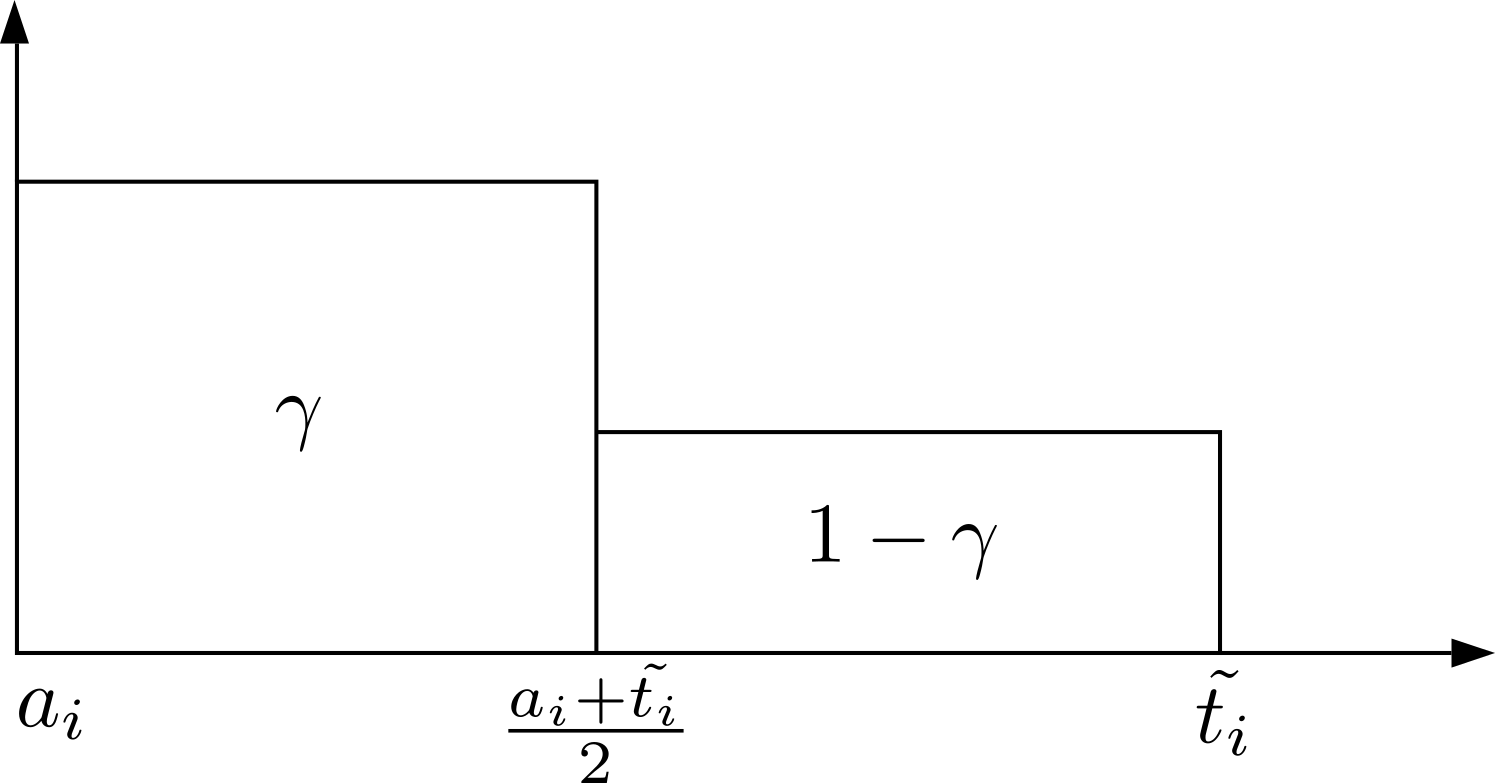
\includegraphics{fig/gendreau2006_distribution.png}
    \caption{Distribuição do limite inferior da janela de tempo de coleta dos
             pedidos \cite{gendreau_neighborhood_2006}}
    \label{fig:gendreau2006_distribution}
\end{figure}

\noindent em que, $\mu$ simboliza a probabilidade do limite inferior da janela 
de tempo de coleta estar contido no intervalo $[\arrivalTime_\request; 
\frac{\arrivalTime_\request + \Tilde{t}_\request}{2}]$, e é definido por:
%
\begin{equation}
  \mu = \uniformDistribution{0,6}{1,0}.
\end{equation}

Já o limite superior da janela de tempo de coleta é definido por:
%
\begin{equation}
    \latestTimeWindow_\originIndex = 
      \earliestTimeWindow_\originIndex 
      + \tau(\planingHorizon - \arrivalTime_\request),
\end{equation}

\noindent em que, $\tau(\planingHorizon - \arrivalTime_\request)$ 
representa uma fração do tempo entre o instante de chegada do pedido e o fim 
do horizonte de planejamento. Assim, $\tau$ é definido por:
%
\begin{equation}
  \tau = \uniformDistribution{\tau^{\min}}{\tau^{\max}},
\end{equation}

\noindent com $\tau^{\min}$ e $\tau^{\max}$ são parâmetros determinados pelo 
usuário, cujos valores podem variar com o tempo e localização.

Uma janela de tempo é gerada da mesma forma para o local de entrega. 
Neste caso a distribuição de probabilidade para a geração do limite inferior 
da janela de tempo de entrega, como mostrado na 
Figura~\ref{fig:gendreau2006_distribution}, é definido sobre o intervalo
$[\earliestTimeWindow_\originIndex 
+ \arcTravelTime{\originIndex}{\destinationIndex}^{\min}, 
\Tilde{t} + \arcTravelTime{\originIndex}{\destinationIndex}^{\min}]$.
Já o limite superior da janela de tempo de entrega é também definido como uma
fração do intervalo de tempo entre o limite inferior da janela de tempo de
entrega e o instante final do horizonte de planejamento.

O tempo de serviço é igual a 5 minutos em cada local de serviço e um pedido é 
aceito somente quando existe no mínimo 30 minutos entre o instante de chegada 
do pedido e o último instante de coleta 
($\latestTimeWindow_\request - \requestArrivalTime \geq 30$). 
Os valores para os parâmetros $\tau$ usados para a geração das janelas de tempo
foram tomados a partir do sorteio de distribuições uniformes 
$\uniformDistribution{0,1}{0,8}$ e $\uniformDistribution{0,3}{1,0}$.

A Tabela~\ref{tab:gendreau2006_instances_characteristics} apresenta algumas
características das instâncias apresentadas por
\textcite{gendreau_neighborhood_2006}

\begin{table}[h]
\footnotesize
    \caption{Características das instâncias DPDPTW de 
             \textcite{gendreau_neighborhood_2006}}
    \label{tab:gendreau2006_instances_characteristics}
    \centering
    \begin{tabular}{lrr|lrr}
        \toprule
         ID & $\planingHorizon$ & $\numberOfRequests$ & 
         ID & $\planingHorizon$ & $\numberOfRequests$ \\
         \midrule
         req\_rapide\_1\_240\_24 & 240 &  84 & 
         req\_rapide\_3\_450\_24 & 450 & 206 \\ 
         req\_rapide\_1\_240\_33 & 240 & 144 & 
         req\_rapide\_4\_450\_24 & 450 & 217 \\
         req\_rapide\_1\_450\_24 & 240 & 169 & 
         req\_rapide\_4\_240\_24 & 240 &  90 \\ 
         req\_rapide\_2\_450\_24 & 450 & 176 &
         req\_rapide\_5\_240\_24 & 240 &  85 \\
         req\_rapide\_2\_240\_24 & 240 &  94 &
         req\_rapide\_5\_240\_33 & 240 & 153 \\
         req\_rapide\_2\_240\_33 & 240 & 112 &
         req\_rapide\_5\_450\_24 & 450 & 202 \\
         req\_rapide\_3\_240\_24 & 240 &  93 &
         req\_rapide\_5\_450\_24 & 450 & 202 \\
         req\_rapide\_3\_240\_33 & 240 & 111 &
                                 &     &     \\
         \bottomrule
  \end{tabular}
\end{table}





\section{Conjunto de instâncias DPDPTW propostas por 
         Mitrovic-Minic e Laporte (2004) e Mitrovic-
         Minic, Krishnamurti e Laporte (2004)}

Composto por dois subconjuntos de instâncias, cada um contendo 30 instâncias de 
100, 30 instâncias de 500 e 30 instâncias de 1000 pedidos.
Estes conjuntos diferem apenas em relação à distribuição e largura das 
janelas de tempo, que dependem do tempo máximo permitido para servir o pedido, 
assumindo que o pedido é coletado no primeiro instante possível, e são dadas 
por:
%
\begin{equation}
    \Gamma = \latestTimeWindow_{\destinationIndex}
              - \earliestTimeWindow_\originIndex.
    \label{eq: mitrovic_maximal_time_allowed}
\end{equation}


Os pedidos são gerados baseados em dados reais coletados em duas companhias de 
correio de médio e grande porte que operam em Vancouver, Canadá.
No primeiro conjunto a distribuição de pedidos é representada por: 
20\% pedidos com $\Gamma$ = 1 h, 30\% pedidos com $\Gamma$ = 2 h e 
50\% pedidos com $\Gamma$ = 4 h.
No segundo conjunto a distribuição é representada por: 10\% dos pedidos com 
$\Gamma$ = 1 h, 20\% dos pedidos com $\Gamma$ = 2 h, 30\% dos pedidos com 
$\Gamma$ = 4 h, 30\% dos pedidos com $\Gamma$ = 6 h 
e 10\% dos pedidos com $\Gamma$ = 8 h.

O horizonte de planejamento é de 10 h, a área de serviço é de $60 \times 60$ 
km$^2$, e a velocidade do veículo é de 60 km/h. 
Os instantes de chegada dos pedidos ocorrem dentro do horizonte de planejamento
de acordo com uma distribuição uniforme contínua e nenhum pedido é conhecido 
a priori,
%
\begin{equation}
  \arrivalTime_\request = \uniformDistribution{0}{\planingHorizon}.
\end{equation}


Um pedido $\request$ é criado através da seguinte sequência de procedimentos: 
(i) gerar o instante de chegada, 
(ii) gerar aleatoriamente as posições de coleta e entrega e 
(iii) gerar um valor para $\Gamma$.
(iv) calcular os limites das janelas de tempo como:
%
\begin{equation}
  \earliestTimeWindow_\originIndex = \arrivalTime_\request,
\end{equation}
%
\begin{equation}
  \latestTimeWindow_{\destinationIndex} = \earliestTimeWindow_\originIndex +
  \Gamma,
\end{equation}
%
\begin{equation}
  \latestTimeWindow_\originIndex = \latestTimeWindow_{\destinationIndex}
  - \arcTravelTime{i}{i+n},
\end{equation}
%
\begin{equation}
  \earliestTimeWindow_{\destinationIndex} = \earliestTimeWindow_\originIndex
  + \arcTravelTime{i}{i+n}.
\end{equation}

Rejeições de pedidos e violações de janelas de tempo não são permitidas. 
Isso é feito possível pelo fato que a quantidade de veículos 
($\vehiclesSetSize$) é considerada ilimitada. 
A frota inicial considerada é de 20, 60 e 80 veículos para as instâncias com 
100, 500 e 1000 pedidos, respectivamente. 
O ponto de início é posicionado em (20, 30) km.





    % Primeiro capitulo de Resultados
    \chapter{Medidas de dinamismo para roteamento dinâmico de veículos}
\label{ch:medidas}
% TODO Introduzir o que seriam medidas e a importância delas para as pesquisas 
% com relação a roteamento dinâmico de veículos

% TODO adicionar outros exemplos de medidas, explicando para que servem

% TODO explicar o porque dinamismo e urgência foram escolhidas

De acordo com o \textcite{michaelis_dinamico_2019}, dinâmico é algo que evolui
permanentemente, mutável, que admite movimento ou mudança.
Portanto, problemas de roteamento dinâmico de veículos são problemas que 
evoluem com o tempo e que se modificam com o a chegada de novas informações 
\cite{psaraftis_dynamic_2015}.

Muitos dos problemas de roteamento do dia-a-dia são problemas de natureza
dinâmica: entrega de encomendas, entrega de comida, serviços de emergência
(ex.: bombeiros), táxis e transporte por aplicativos. 
Entretanto, estes problemas apresentam diferenças em suas características 
dinâmicas. 

Analisando com atenção percebe-se que existem problemas em que o número de
pedidos agendados (não dinâmicos) é grande quando comparado com os demais
problemas, um exemplo disso é o problema de entrega de encomendas, muitas das
entregas são conhecidas \textit{a priori}, entretanto, algumas encomendas de
emergência podem aparecer durante o período de operação.
Em contrapartida, existem problemas em que todos os pedidos são dinâmicos e
devem ser atendidos com a maior rapidez possível, como por exemplo os serviços
de bombeiros.
Existem também os casos intermediários, em que pedidos podem surgir em forma de
agendamento antecipado ou dinamicamente entretanto não existe urgência para o
cumprimento destes.
A entrega de alimentos, por exemplo, é um problema deste tipo.

Percebendo que estas diferentes características nos problemas dinâmicos eram 
também associadas a diferenças nas qualidades das soluções encontradas,
muitos pesquisadores tentaram criar medidas de dinamismo de forma a 
possibilitar a classificação de problemas e auxiliar na escolha de métodos de 
solução.

A Seção~\ref{sec:medidas_revisao} dedica-se a relatar algumas das medidas de
dinamismo propostas na área de roteamento dinâmico de veículos,
além de relatar alguns dos usos práticos dessas medidas. 
Posteriormente, a Seção~\ref{sec:medidas_van_lon} apresenta a definição das
medidas de dinamismo e urgência propostas por \textcite{van_lon_measures_2016}.
No Capítulo~\ref{ch:analise} usa-se estas medidas para analisar
e comparar os conjuntos de instância de \textit{benchmark} expostos no 
Capítulo~\ref{ch:instancias}.








\section{Revisão bibliográfica}\label{sec:medidas_revisao}

Proposta primeiramente por \citeonline{lund_vehicle_1996}, o grau de dinamismo
de uma instância de qualquer VRP dinâmico representa a razão entre a quantidade
de pedidos dinâmicos, que se fazem conhecidos em um instante
$\arrivalTime_\request > 0$, e a quantidade total de pedidos da instância:
%
\begin{equation}
  \degreeOfDynamism = \frac{\numberOfRequests_{\text{d}}}{\numberOfRequests},
  \label{eq:degreeOfDynamism}
\end{equation}

\noindent em que $\degreeOfDynamism$ é o grau de dinamismo e 
$\numberOfRequests_{d}$ o número de pedidos dinâmicos

Essa classificação proporcionou uma base para o estudo das relações entre o 
grau de dinamismo, os tipos de métodos usados para a solução dos 
problemas e as características das soluções obtidas.
\citeonline{wong_dynamic_2014}, por exemplo, mostram que existe uma relação não
linear entre o grau de dinamismo e o custo de transporte de uma instância de um
problema responsivo à demanda.
Suas análises numéricas elucidam a existência de um pico de ineficiência para
vários algoritimos heurísticos quando $\degreeOfDynamism \approx 0{,}7$, o que
os autores classificaram como ``zona de dilema''.
Através dessa descoberta \citeonline{wong_dynamic_2014} descrevem uma série de
políticas para que operadores de sistemas de transporte responsivos à demanda
(DRT - \textit{Dynamic Responsive Transpot}) possam seguir para permanecer 
longe da ``zona de dilema''.

Similarmente, \citeonline{larsen_partially_2002} usam essa mesma medida de 
grau de dinamismo para estudar a relação entre o custo de rota para o 
problema parcialmente dinâmico do reparador itinerante 
(PDTRP - \textit{Partially Dynamic Traveling Repairman Problem}).
Os resultados empíricos ilustram uma relação linear entre o nível de
dinamismo de uma instância e o custo da rota de um sistema relativamente ativo.

Posteriormente, baseando-se no fato de que o instante de chegada dos pedidos
dinâmicos também deve afetar o grau de dinamismo,
\textcite{larsen_dynamic_2000} define o grau efetivo de dinamismo por:
%
\begin{equation}
  \eDegreeOfDynamism = 
  \frac{1}{\numberOfRequests}
  \sum_{\request \in \requests}
  {
    \frac{\arrivalTime_\request}{\planingHorizon}
  },
  \label{eq:eDegreeOfDynamism}
\end{equation}

\noindent em que $\eDegreeOfDynamism$ é o grau efetivo de dinamismo e 
representa a média da razão entre os instantes que os pedidos são conhecidos 
quando comparados com o último instante possível para a chegada deles, 
$\planingHorizon$, no caso. Os instantes de chegada dos pedidos estáticos são 
considerados igual a zero.

É importante destacar que apesar de representarem formas de cálculo diferentes,
o grau de dinamismo e o grau de dinamismo efetivo compartilham entre si o mesmo
intervalo de possíveis valores, contido entre $0$ e $1$, sendo que
$\degreeOfDynamism = \eDegreeOfDynamism = 0$ classifica uma instância
totalmente estática e $\degreeOfDynamism = \eDegreeOfDynamism = 1$ representa
uma totalmente dinâmica.

Em um outro estudo, \citeonline{larsen_classification_2007} usam o grau efetivo
de dinamismo para classificar os problemas de roteamento dinâmico de veículos
(DVRP - \textit{Dynamic Vehicle Routing Problem}) em três classes distintas:
fracamente, moderadamente e fortemente dinâmicos, cujos intervalos de valores 
$\eDegreeOfDynamism$ correspondem, respectivamente, a $\eDegreeOfDynamism \leq
0{,}3$, $0{,}3  < \eDegreeOfDynamism < 0{,}8$ e $0{,}8 \leq
\eDegreeOfDynamism$.
A intenção dessa segregação de problemas é facilitar a escolha de um algoritmo
para a sua solução.

\citeonline{larsen_dynamic_2000} também estende o grau de dinamismo efetivo
para problemas com janelas de tempo.
A ideia é contabilizar também o nível de urgência de cada um dos pedidos, 
sendo que o nível de urgência é visto como o tempo de reação disponível
para que o sistema, após receber a informação do pedido no instante
$\arrivalTime_\request$, possa passar pelo nó de coleta $\originNode$
antes do limite superior da janela de tempo de coleta
$\latestTimeWindow_{\originIndex}$.
\citeonline{larsen_dynamic_2000} define que: 
%
\begin{equation}
  \reactionTime_\request = \latestTimeWindow_{\originIndex}
                           - \arrivalTime_\request,
\end{equation}

\noindent em que $\reactionTime_\request$ é o tempo de reação do pedido
$\request$.

Com isso, o grau efetivo de dinamismo, quando contabilizado o tempo de reação,
é definido por \cite{larsen_dynamic_2000}:
%
% TODO tentar alinhar os sinais de igualdade das duas equações a seguir
%
\begin{equation}
  \eDegreeOfDynamismTW = 
  \frac{1}{\numberOfRequests}
  \sum_{\request \in \requests}
  {
    \left(
    \frac{\planingHorizon - (\latestTimeWindow_\originIndex
                             - \arrivalTime_\request)}
         {\planingHorizon}
    \right),
  }
\end{equation}

\begin{equation}
  \eDegreeOfDynamismTW = 
  \frac{1}{\numberOfRequests}
  \sum_{\request \in \requests}
  {
    \left(
      1 - \frac{\reactionTime_\request}{\planingHorizon}
    \right),
  }
\end{equation}

\noindent em que $\eDegreeOfDynamismTW$ é o grau efetivo de dinamismo com 
janelas de tempo.

É importante destacar que, assim como as medidas apresentadas anteriormente, o
grau efetivo de dinamismo com janelas de tempo também apresenta valores somente
dentro do intervalo $[0, 1]$.

\citeonline{pillac_review_2013} relata que todas as três medidas expostas neste
capítulo se provaram úteis para capturar os aspectos do dinamismo relacionados
com o tempo.
Entretanto essas medidas não levam em consideração outras fontes de dinamismo,
como a distribuição espacial dos pedidos e o tempo de viagem entre pedidos.
Essas fontes de dinamismo se mostram bastante importantes quando o objetivo é
minimizar o tempo de resposta do sistema.

Além disso, apesar de não considerada na definição das medidas de dinamismo, a
frequência com que os pedidos chegam ao sistema tem um grande impacto no tempo
disponível para otimização \cite{pillac_review_2013}.
Similarmente, \citeonline{kilby_dynamic_1998} fazem a observação de que a
frequência dos pedidos influencia a quantidade de vezes que o algoritmo
precisa ser executado.
Eles destacam que instâncias em que os pedidos estão agrupados em
pequenos intervalos de tempo geram menos necessidade de mais rodadas de
otimização do que casos onde os pedidos estão separados um dos outros de 
maneira uniforme.

No final do seu artigo, \citeonline{larsen_classification_2007} recomendam
para futuras pesquisas a extensão do grau de dinamismo para que ele também 
leve em conta outras características do problema, como o tamanho dos tempos de 
serviço e o carregamento dos pedidos.
Eles também mencionam que é desafiador encontrar uma medida única com
capacidade de apreender múltiplas características de uma instância.






\section{Medida de dinamismo e urgência proposta por Van Lon, Ferrante et al.
         (2016)}\label{sec:medidas_van_lon}
Com o intuito de produzir medidas que melhor representam as características
relacionadas ao dinamismo de um DPDPTW, \citeonline{van_lon_measures_2016} 
propõem uma nova definição para a medida de dinamismo, como também uma nova
medida denominada urgência.
Apesar do foco ser em problemas DPDPTW, \citeonline{van_lon_measures_2016}
afirmam que os conceitos de dinamismo e urgência não são limitados a este tipo
de problema, podendo ser usados em qualquer DVRP.

Como premissa, os autores consideram que estes parâmetros devem ser 
relacionados apenas ao problema, e portanto, o algoritmo usado para solução 
não deve influenciar em seus valores.
Entretanto, é desejado que essas medidas colaborarem para a classificação das 
instâncias e assim permitam a análise da eficácia dos algoritmos quando 
submetidos a diferentes condições de dinamismo e urgência. 
Além disso, \citeonline{van_lon_measures_2016} afirmam que as medidas devem ser 
interdependentes, não podendo haver correlação entre suas definições. 

O restante desse capítulo apresenta a definição, feita por
\citeonline{van_lon_measures_2016}, das duas medidas usadas para a determinação
das características temporais dos pedidos de uma instância de um problema de 
roteamento dinâmico qualquer.






\subsection{Dinamismo}\label{sec:dinamismo}
Define-se, primeiramente, que o grau de dinamismo é dado através da 
continuidade de mudança das informações presentes para um sistema. 
Por esse ponto de vista, todo evento que introduz informações novas para o 
problema, como a chegada de um pedido, a quebra de um veículo ou o cancelamento
de uma viagem, é classificado como uma mudança.
Um cenário muito dinâmico é caracterizado por mudanças contínuas, em oposição a
um cenário pouco dinâmico, onde mudanças ocorrem ocasionalmente.
A Figura~\ref{fig:van_lon_measures_2016_dynamism} demonstra, 
através de exemplos, as diferentes formas de distribuição de mudanças,
associando cada uma à um grau de dinamismo.

% TODO: mudar para arquivo .eps
\begin{figure}[H]
    \begin{center}
        \makebox[\textwidth]
          {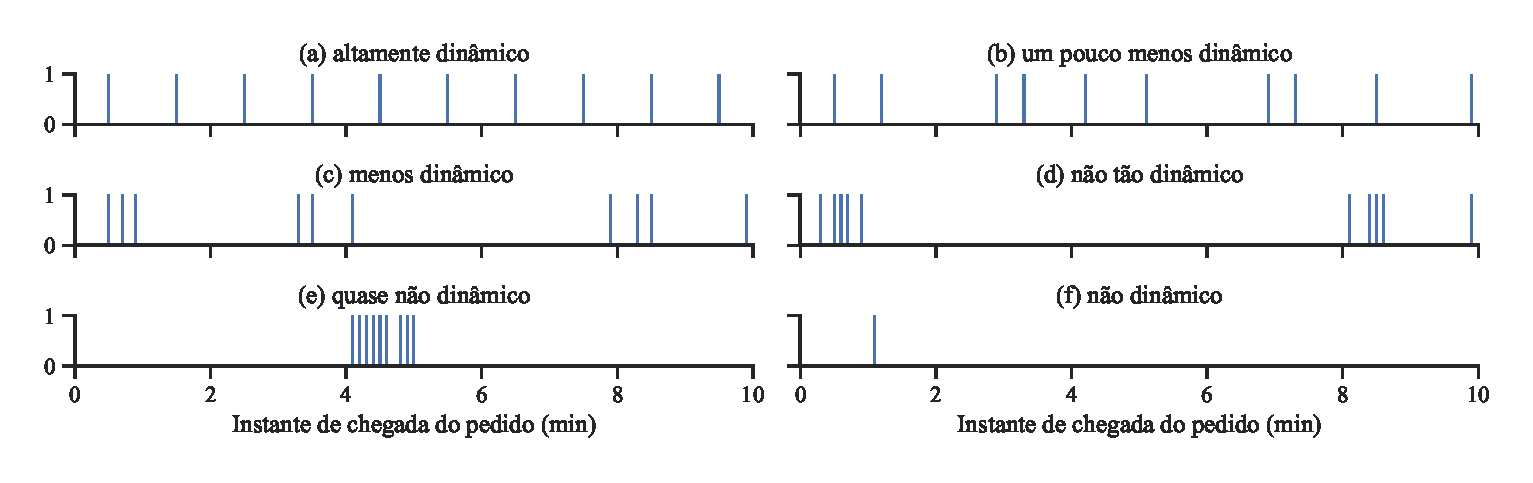
\includegraphics[width=\textwidth]{./fig/dynamism_sample.eps}}
        \caption{Exemplos de cenários com diferentes valores de dinamismo 
        \cite{van_lon_measures_2016}}
        \label{fig:van_lon_measures_2016_dynamism}
    \end{center} 
\end{figure}

Todos os gráficos da Figura~\ref{fig:van_lon_measures_2016_dynamism},
identificados pelas letras (a-f), representam um cenário com horizonte de 
planejamento de 10 minutos e com um total de 10 pedidos dinâmicos.
No cenário da Figura~\ref{fig:van_lon_measures_2016_dynamism}(a) os eventos 
acontecem em intervalos igualmente espaçados e distribuídos proporcionalmente 
no horizonte de planejamento.
Nos cenários da Figura~\ref{fig:van_lon_measures_2016_dynamism}(b, c) 
pode-se ver que mudanças ocorrem de maneira menos distribuída, apresentando uma
leve concentração de pedidos.
Na Figura~\ref{fig:van_lon_measures_2016_dynamism}(d, e) todos os eventos
ocorrem em uma ou duas bateladas, diminuindo ainda mais a distribuição dos
pedidos e, com isso, diminuindo o dinamismo dos cenários.
Na Figura~\ref{fig:van_lon_measures_2016_dynamism}(f) todos os eventos chegam
em um mesmo instante, resultando em um cenário sem dinamismo
\cite{van_lon_measures_2016}.

Para formular a medida de dinamismo \citeonline{van_lon_measures_2016} definem
primeiramente uma lista, $\intervalsBetweenArrivals$, de intervalos de chegadas
entre pedidos:
%
\begin{equation}
    \intervalsBetweenArrivals = 
    \{\intervalBetweenArrivals_0,\intervalBetweenArrivals_1,\ldots, 
    \intervalBetweenArrivals_{\numberOfRequests-2}\} = 
    \{\arrivalTime_j - \arrivalTime_i 
    \mid j = i + 1 \wedge \forall i, j \in \pickupNodes\},
    \label{eq:van_lon_measures_2016_intervalsBetweenArrivals}
\end{equation}
%
\begin{equation}
    |\intervalsBetweenArrivals| = \numberOfRequests - 1.
    \label{eq:van_lon_measures_2016_intervalsBetweenArrivalsSize}
\end{equation}

\noindent em que $\intervalsBetweenArrivals$ é a lista de intervalos entre 
chegada de pedidos e $\intervalBetweenArrivals_\request$ o intervalo de tempo 
entre a chegada do pedido $\request$ e seu sucessor. 
Portanto, $\intervalsBetweenArrivals$ representa uma lista com todos os valores
de intervalos de tempo em que o estado do sistema não é alterado, ordenados
cronologicamente.
Essa lista possui uma quantidade de valores $|\intervalsBetweenArrivals|$ 
cuja definição é (\ref{eq:van_lon_measures_2016_intervalsBetweenArrivalsSize}).

Para fins de comparação, é definido um intervalo de chegada perfeito,
$\perfectInterval$. Este é dado por:
%
\begin{equation}
    \perfectInterval = \frac{H}{\numberOfRequests},
    \label{eq:van_lon_measures_2016_perfectInterval}
  \end{equation}

\noindent em que $\perfectInterval$ é o intervalo de chegada perfeito.

Com isso obtêm-se o espaço de tempo entre pedidos do cenário com maior
dinamismo possível, dada uma quantia de pedidos $\numberOfRequests$ 
e um horizonte de planejamento $\planingHorizon$.
Voltando ao exemplo da Figura~\ref{fig:van_lon_measures_2016_dynamism},
temos que o cenário (a) seria o cenário em que
$\intervalBetweenArrivals_\request = \perfectInterval, \forall
\intervalBetweenArrivals_\request \in \intervalsBetweenArrivals$.
Ou seja, dos cenários apresentados na 
Figura~\ref{fig:van_lon_measures_2016_dynamism}, o cenário (a) é, além do mais
dinâmico dos cenários da figura, também o cenário mais dinâmico possível pra
esses valores de $\numberOfRequests$ e $\planingHorizon$.

Tendo os conceitos de intervalos entre chegadas de pedido e o intervalo de
chegada perfeito definidos, pode-se definir o desvio,
$\deviationFromPerfectInterval$, entre os intervalos de chegada contidos em
$\intervalsBetweenArrivals$ com o intervalo de chegada perfeito,
$\perfectInterval$:
%
\begin{equation}
    \deviationFromPerfectInterval_i =
        \begin{cases}
            \perfectInterval - \intervalBetweenArrivals_i,
            & \text{se $i = 0$ 
                    e $\intervalBetweenArrivals_i < \perfectInterval$} \\
            \perfectInterval - \intervalBetweenArrivals_i 
            + \frac{\perfectInterval-\intervalBetweenArrivals_i}
                   {\perfectInterval}
            \cdot \deviationFromPerfectInterval_{i-1},
            & \text{se $i > 0$ 
                    e $\intervalBetweenArrivals_i < \perfectInterval$} \\
            0, & \text{caso contrário},
        \end{cases}
    \label{eq:van_lon_measures_2016_deviationFromPerfectInterval}
\end{equation}

\noindent em que $\deviationFromPerfectInterval_i$ é o desvio 
entre os intervalos de chegada $\intervalBetweenArrivals_i$ e o 
$\perfectInterval$. 
O termo ($\frac{\perfectInterval-\intervalBetweenArrivals_i}
{\perfectInterval} \cdot \deviationFromPerfectInterval_{i-1}$) serve para 
penalizar, de forma recursiva, a aglutinação de eventos em pequenos 
períodos de tempo.

% TODO: explicar melhor o que significa cada um dos casos da equação acima,
% assim como o conceito completo expresso por ela.

Consequentemente, o desvio total do cenário pode ser calculado por:
%
\begin{equation}
    \deviation = 
    \sum_{i=0}^{|\intervalsBetweenArrivals|} \deviationFromPerfectInterval_i.
    \label{eq:van_lon_measures_2016_totalDeviationFromPerfectInterval}
\end{equation}

Entretanto, faz-se necessária a normalização do desvio total do cenário com
relação ao desvio máximo possível.
Para isso, calcula-se o maior valor:
%
\begin{equation}
    \maxDeviation =
    \sum_{i=0}^{|\intervalsBetweenArrivals|} 
		\overline{\deviationFromPerfectInterval}_i,
    \label{eq:van_lon_measures_2016_bigestTotalDeviationFromPerfectInterval}
\end{equation}

\noindent em que:
%
\begin{equation}
    \overline{\deviationFromPerfectInterval}_i = \perfectInterval + 
        \begin{cases}
            \frac{\perfectInterval - \intervalBetweenArrivals_i}
								 {\perfectInterval} 
						\cdot \deviationFromPerfectInterval_{i-1},
						& \text{se $i>0$ e $\intervalBetweenArrivals_i 
                    < \perfectInterval$}\\
            0, & \text{caso contrário.}
        \end{cases}
    \label{eq:van_lon_measures_2016_bigestDeviationFromPerfectInterval}    
\end{equation}

Combinando  
(\ref{eq:van_lon_measures_2016_bigestTotalDeviationFromPerfectInterval})
e~(\ref{eq:van_lon_measures_2016_bigestDeviationFromPerfectInterval}), define-se 
dinamismo como:

\begin{equation}
      \dynamism = 1 - \frac{\deviation}{\maxDeviation} = 1 -
      \frac{\sum_{i=0}^{|\intervalsBetweenArrivals|}
			\deviationFromPerfectInterval_i}{\sum_{i=0}^{|\intervalsBetweenArrivals|}
      \overline{\deviationFromPerfectInterval}_i}.
      \label{eq:van_lon_measures_2016_dynamism}
\end{equation}

% TODO: Escrever interpretação das 4 equações anteriores






\subsection{Urgência}\label{sec:urgencia}

No contexto dos DVRPs, a urgência representa o tempo de reação disponível ao 
sistema de transporte para que ele consiga atender a um pedido.
Essa medida pode ser expressa através de unidades de tempo e definida pela 
diferença entre o instante de chegada de um pedido ($\arrivalTime_\request$) 
e o limite superior da janela de tempo de coleta 
($\latestTimeWindow_\originIndex$).
A Figura~\ref{fig:van_lon_measures_2016_urgency} exemplifica dois casos.

%TODO: converter imagem de png para eps
\begin{figure}[H]
    \begin{center}
        \makebox[\textwidth]{
          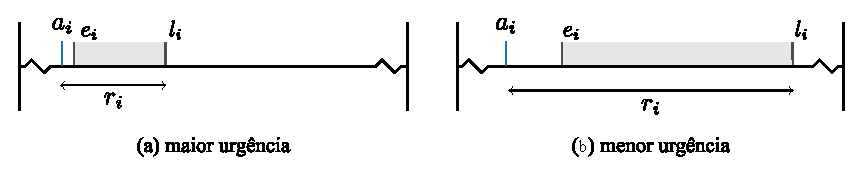
\includegraphics[width=\textwidth]{fig/urgency_sample.eps}}
        \caption{Exemplos de pedidos com diferentes valores de urgência 
                 \cite{van_lon_measures_2016}}
        \label{fig:van_lon_measures_2016_urgency}
    \end{center} 
\end{figure}

No cenário da Figura~\ref{fig:van_lon_measures_2016_urgency}(a) temos o exemplo
de um pedido com grande urgência, ou seja, menor tempo de reação.
Já no caso da Figura~\ref{fig:van_lon_measures_2016_urgency}(b) o tempo de 
reação é maior, portanto o pedido é menos urgente.

Baseando-se na Figura~\ref{fig:van_lon_measures_2016_urgency}, 
\citeonline{van_lon_measures_2016} define urgência por:
%
\begin{equation}
    \urgency_\request = 
    \reactionTime_\request =
    \latestTimeWindow_\request - \arrivalTime_\request,
    \label{eq:van_lon_measures_2016_urgency}
\end{equation}

\noindent em que $\urgency_\request$ é a urgência do pedido $\request$.

Para obter uma indicação da urgência de um cenário completo, pode-se computar a
média e o desvio padrão das urgências. 
Esta definição é similar ao grau de dinamismo efetivo com janelas de tempo 
proposto por \citeonline{larsen_dynamic_2000} e definido por
(\ref{eq:degreeOfDynamism})~e~(\ref{eq:eDegreeOfDynamism}).
Entretanto, existe uma diferença entre estas duas definições.
\citeonline{larsen_dynamic_2000} normaliza os valores do grau de dinamismo
efetivo com janelas de tempo usando o horizonte de planejamento.  
Já \citeonline{van_lon_measures_2016} acredita que a extensão do cenário e
a urgência devem ser independentes.




    % Segundo capitulo de Resultados
    \chapter{Análise dos Conjuntos de \textit{Benchmark}}\label{ch:analise}

Neste capítulo as métricas apresentadas no Capítulo~\ref{ch:medidas} são 
utilizadas para analisar as instâncias de \textit{benchmark} descritas no
Capítulo~\ref{ch:instancias}. 
Esta análise tem como objetivo avaliar a dispersão dos valores de dinamismo e 
urgência das instâncias de cada conjunto de \textit{benchmark} e com isso 
permitir que futuras pesquisas possam se basear nos
dados expostos nesse capítulo para escolher conjuntos de \textit{benchmark} que
representem cenários de interesse prático para teste.






\section{Distribuição do grau de dinamismo e da urgência}

Cada um dos gráficos apresentados na 
Figura~\ref{fig:scatterplot_instance_planing_horizon} representa um conjunto 
de instâncias de \textit{benchmark} diferente. 
Cada ponto no gráfico corresponde aos valores de urgência média normalizada 
(eixo vertical) e dinamismo (eixo horizontal) de uma das instâncias desse 
conjunto.
A normalização da urgência média é feita de maneira que o valor zero represente
uma urgência média igual a zero e o valor um represente a maior urgência média
encontrada dentro do conjunto de instâncias de \textit{benchmark} em questão.
A figura mostra o acúmulo dos pontos, o que demonstra a falta
de diversidade entre instâncias de um mesmo conjunto de \textit{benchmark},
para os critérios considerados.

% TODO Rodrigo: porque o que está relatado no parágrafo anterior é ruim?

A Figura~\ref{fig:dynamism_boxplot_planing_horizon} mostra os mesmos valores de
dinamismo exibidos na Figura~\ref{fig:scatterplot_instance_planing_horizon}, 
entretanto em forma de diagrama de caixas, em que 50\% dos valores de dinamismo
de cada conjunto de \textit{benchmark} estão contidos nas caixas.
A mediana dos valores é demarcada por um risco vertical dentro desta caixa e os
limites inferiores ($LI$) e superiores ($LS$) são demarcados pelos segmentos 
de reta vertical externos às caixas, cujos valores podem ser calculados 
por:
%
\begin{equation}
  LI = Q_1 - 1{,}5 \cdot AIQ,
\end{equation}
%
\begin{equation}
  LS = Q_3 + 1{,}5 \cdot AIQ,
\end{equation}
%
\begin{equation}
  AIQ = Q_3 - Q_1,
\end{equation}

\noindent em que $Q_1$ é o primeiro quartil, correspondendo a 25\% das menores 
medidas, $Q_3$ é o terceiro quartil, correspondendo a 75\% das menores medidas
e $AIQ$ é a amplitude interquartil. Ainda no gráfico de caixas, podem ser 
encontrados pequenos losangos, indicando valores não contidos no intervalo 
$[LI; LS]$.

Pode-se observar que quatro dos seis conjuntos estudados possuem medianas 
menores que 0,1 e uma alta concentração de instâncias com dinamismo menor que 
0,2, indicando uma falta de diversificação das instâncias desses quatro 
conjuntos. 
Vale destacar que quanto maior o dinamismo, maior a quantidade de vezes que
necessita-se usar o algoritmo de otimização.
Portanto, conjuntos de \textit{benchmark} com baixo valor de dinamismo podem
beneficiar algoritmos que retornem bons resultados a custo de um longo tempo de
computação.

Outro fator interessante a se destacar é a escassez de instâncias com dinamismo
entre 0,45 e 0,6. 
\citeonline{van_lon_measures_2016} afirmam que este intervalo de valores de 
dinamismo ocorre em cenários gerados por distribuições Poisson homogêneas.
Tendo em vista que as chegadas de pedidos de viagem em sistemas de 
\textit{dial-a-ride} acontecem de forma a se assemelhar com uma distribuição de
Poisson homogênea \cite{schilde_metaheuristics_2011}, a falta de instâncias 
com esses valores de dinamismo prejudica a análise de cenários realísticos.

% TODO mudar imagem para .eps
\begin{figure}[H]
    \centering
    \makebox[\textwidth]
    {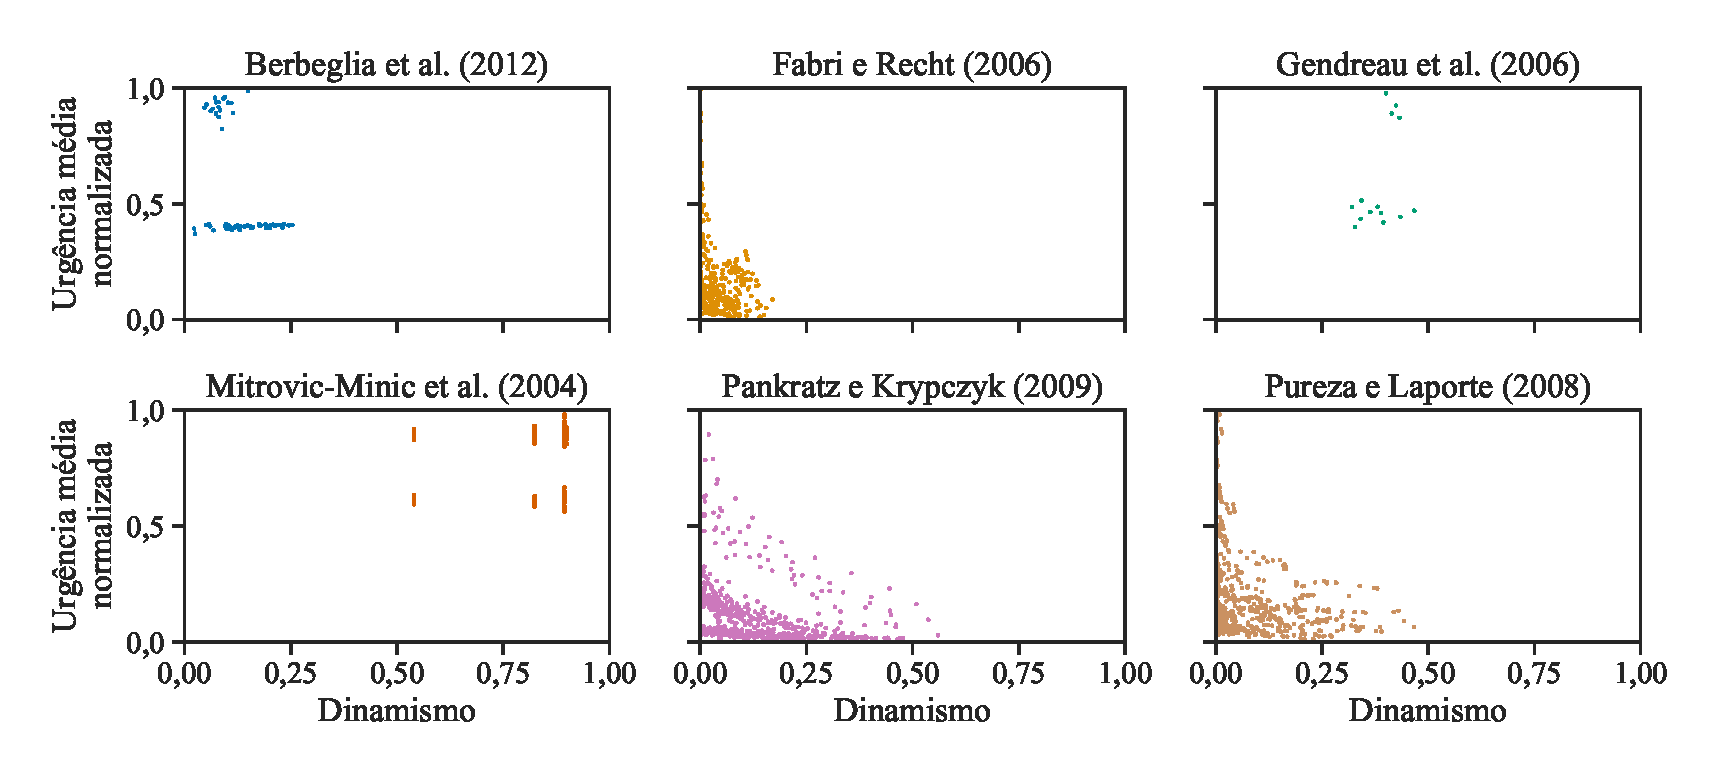
\includegraphics[width=\textwidth]
    {fig/analyses/scatterplot_dynamism_x_urgency_mean_norm_max_planing_horizon.eps}}
    \caption{Gráfico de dispersão da urgência média e do dinamismo de cada 
    conjunto de \textit{benchmark}}
    \label{fig:scatterplot_instance_planing_horizon}
\end{figure}

% TODO mudar imagem para .eps
\begin{figure}[H]
    \centering
    \makebox[\textwidth]
    {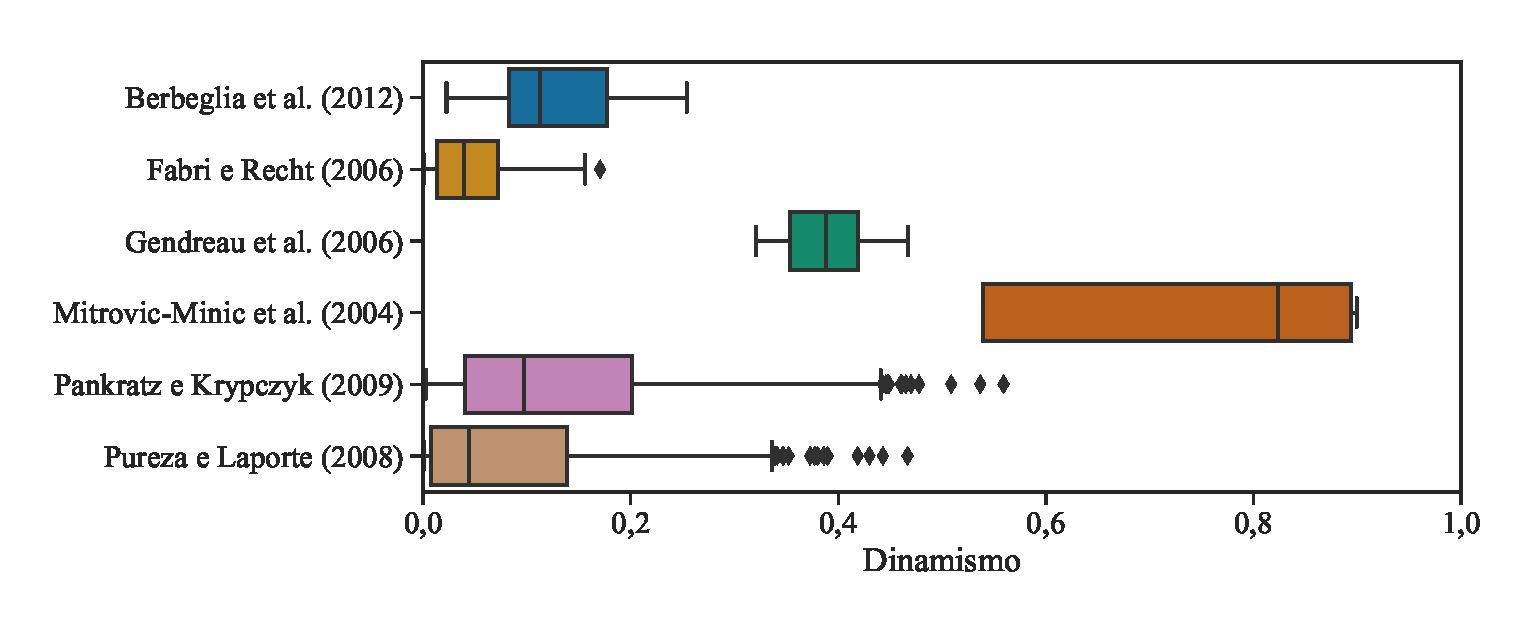
\includegraphics[width=\textwidth]
    {fig/analyses/boxplot_dynamism_by_benchmark_planing_horizon.eps}}
    \caption{Diagrama de caixa dos valores de dinamismo por \textit{benchmark}}
    \label{fig:dynamism_boxplot_planing_horizon}
\end{figure}





\section{Correlação entre os limites inferiores das janelas de tempo de coleta 
e os instantes de chegada dos pedidos}

Pela definição de dinamismo apresentada na Seção~\ref{sec:dinamismo}, os 
intervalos entre os instantes de chegada dos pedidos são os principais fatores
determinadores do valor de dinamismo de uma instância.
Portanto, para que um conjunto de \textit{benchmark} possua instâncias cujos 
valores de dinamismo sejam distintos entre si, se faz necessário que a 
distribuição dos instantes de chegada seja diferente entre instâncias 
\cite{van_lon_measures_2016}.

Entretanto, no Capítulo~\ref{ch:instancias}, percebe-se que grande parte dos 
conjuntos de \textit{benchmark} apresentados possuem um único método de 
dinamização, não possibilitando a diversificação do tamanho dos intervalos de 
tempo entre instâncias.
A única exceção é o método de \citeonline{pankratz_benchmark_2009} que varia o 
valor $\maneuverTime$ garantido a geração de instâncias cujos instantes de 
chegadas diferem entre si.
Porém, mesmo variando esse valor, não foi alcançada uma dispersão grande 
dos valores de dinamismo entre cenários 
(Figuras~\ref{fig:scatterplot_instance_planing_horizon}~e
\ref{fig:dynamism_boxplot_planing_horizon}).

Dentre os métodos de dinamização apresentados no Capítulo~\ref{ch:instancias} é 
comum a utilização dos limites da janela de tempo de coleta para o cálculo dos 
instantes de chegada dos pedidos.
O objetivo do uso deste parâmetro na hora de computar o instante de chegada do 
pedido é garantir que os pedidos possam ser atendidos em tempo hábil.
Entretanto, isso faz com que a distribuição das janelas de tempo das instâncias
estáticas influenciem altamente na distribuição dos instantes de chegadas nos 
pedidos.
Portanto, se a distribuição dos limites das janelas de tempo possuir acúmulo 
de valores, pode-se esperar que os instantes de chegada dos pedidos também  
possua o mesmo acúmulo.

% TODO Rodrigo: pouco visual. Exemplo?

As Figuras~\ref{fig:hist_pickup_lower_tw}~e~\ref{fig:hist_pickup_upper_tw} 
apresentam a distribuição dos limites inferiores e superiores das janelas de 
tempo de coleta de cada um dos conjuntos de \textit{benchmark} normalizados 
pelos horizontes de planejamento de suas respectivas instâncias.
Nota-se que os limites inferiores tendem, em sua maioria, a acumular no início 
do horizonte de planejamento.
Já os limites superiores possuem uma distribuição menos aglutinada, 
porém apresentando ainda pontos de concentração.

\begin{figure}[h]
    \centering
    \makebox[\textwidth]
    {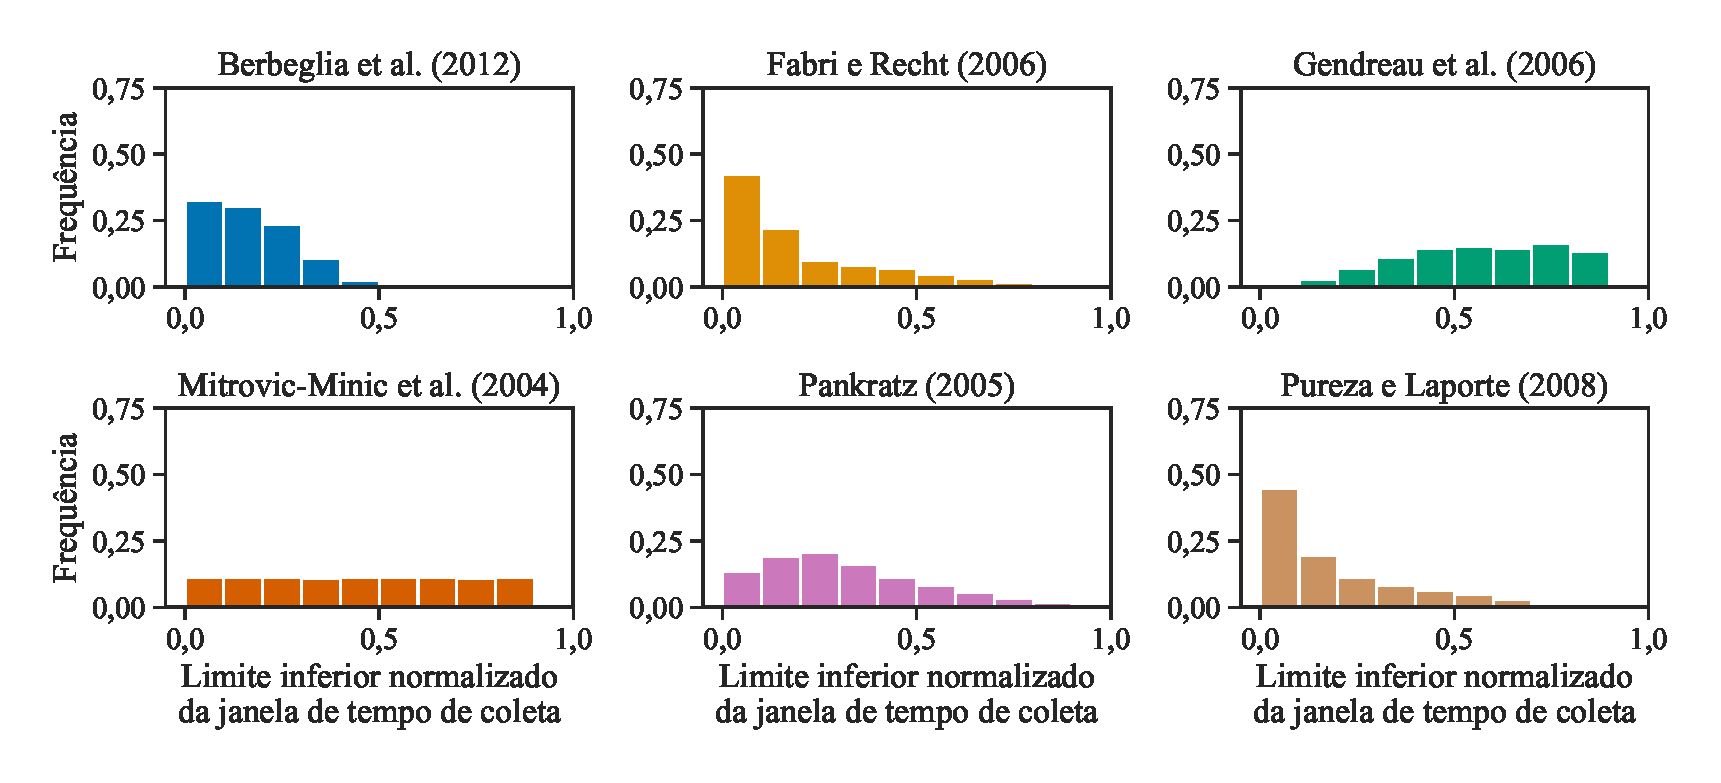
\includegraphics[width=\textwidth]
    {fig/analyses/hist_real_pltw_norm_h_by_benchmark_planing_horizon.eps}}
    \caption{Histograma dos limites inferiores das janelas de tempo 
             de coleta por conjunto de \textit{benchmark}}
    \label{fig:hist_pickup_lower_tw}
\end{figure}

\begin{figure}[h]
    \centering
    \makebox[\textwidth]
    {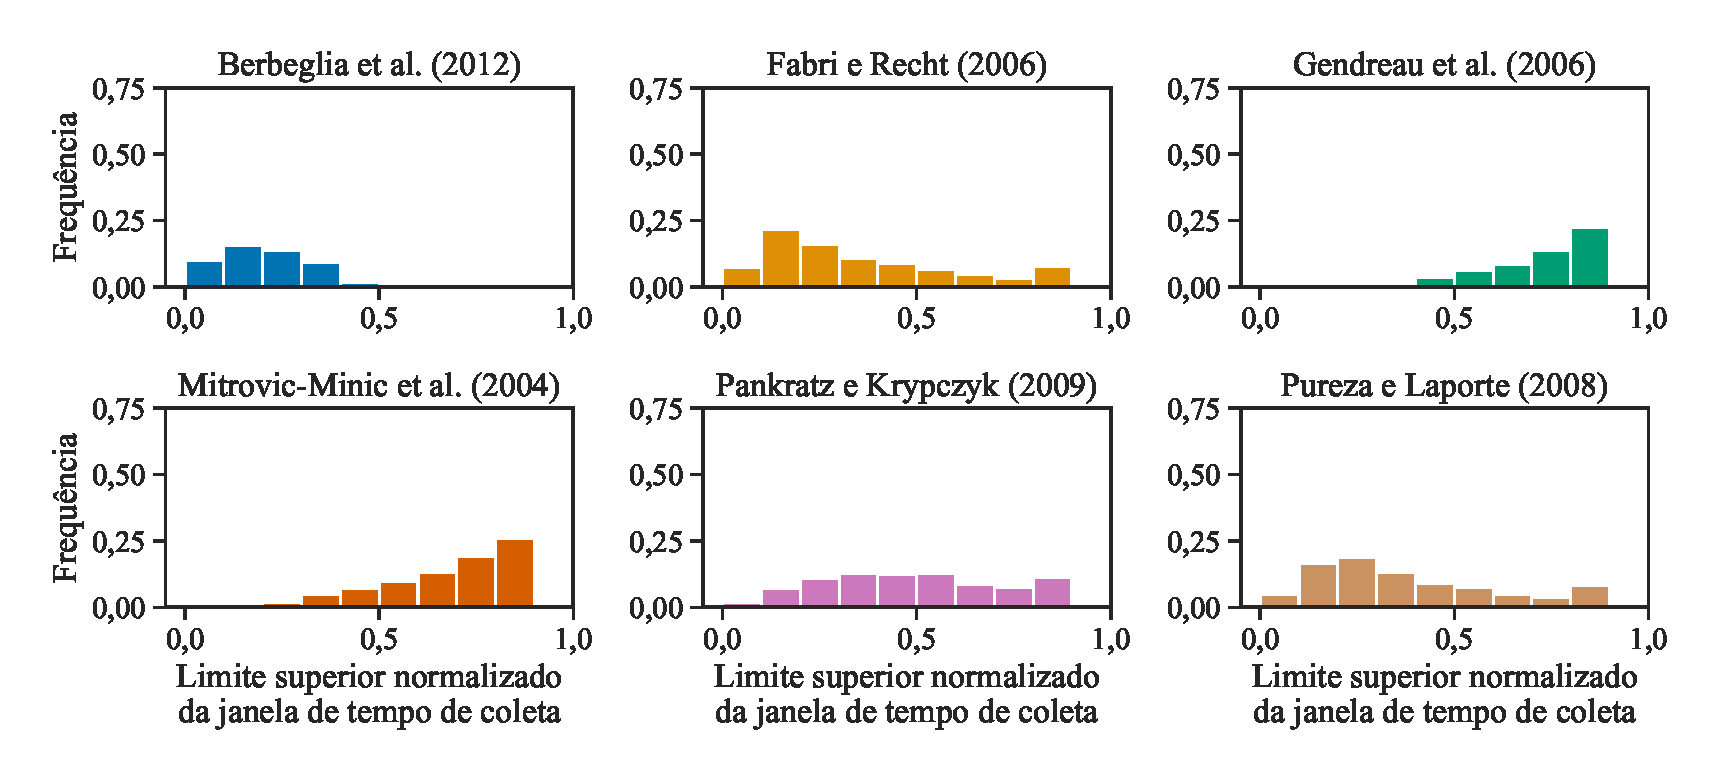
\includegraphics[width=\textwidth]
    {fig/analyses/hist_putw_norm_h_by_benchmark_planing_horizon.eps}}
    \caption{Histograma dos limites superiores das janelas de tempo de 
             coleta por conjunto de \textit{benchmark}}
    \label{fig:hist_pickup_upper_tw}
\end{figure}

% TODO Rodrigo: o que tem a ver com as características das instâncias?
% com técnica de dinamização

Como discutido anteriormente, esse acúmulo dos limites da janela de coleta pode
ser propagado para a distribuição dos instantes de chegadas.
Essa propagação pode ser visualizada na Figura~\ref{fig:hist_arrival_time}, que
apresenta as distribuições dos instantes de chegada dos pedidos.
Observa-se que alguns dos acúmulos apresentados nas 
Figuras~\ref{fig:hist_pickup_lower_tw}~e~\ref{fig:hist_pickup_upper_tw} podem 
ser também observados na Figura~\ref{fig:hist_arrival_time}.

% TODO Rodrigo: O que isso quer dizer? Como é feita a propagação?

\begin{figure}[h]
    \centering
    \makebox[\textwidth]
    {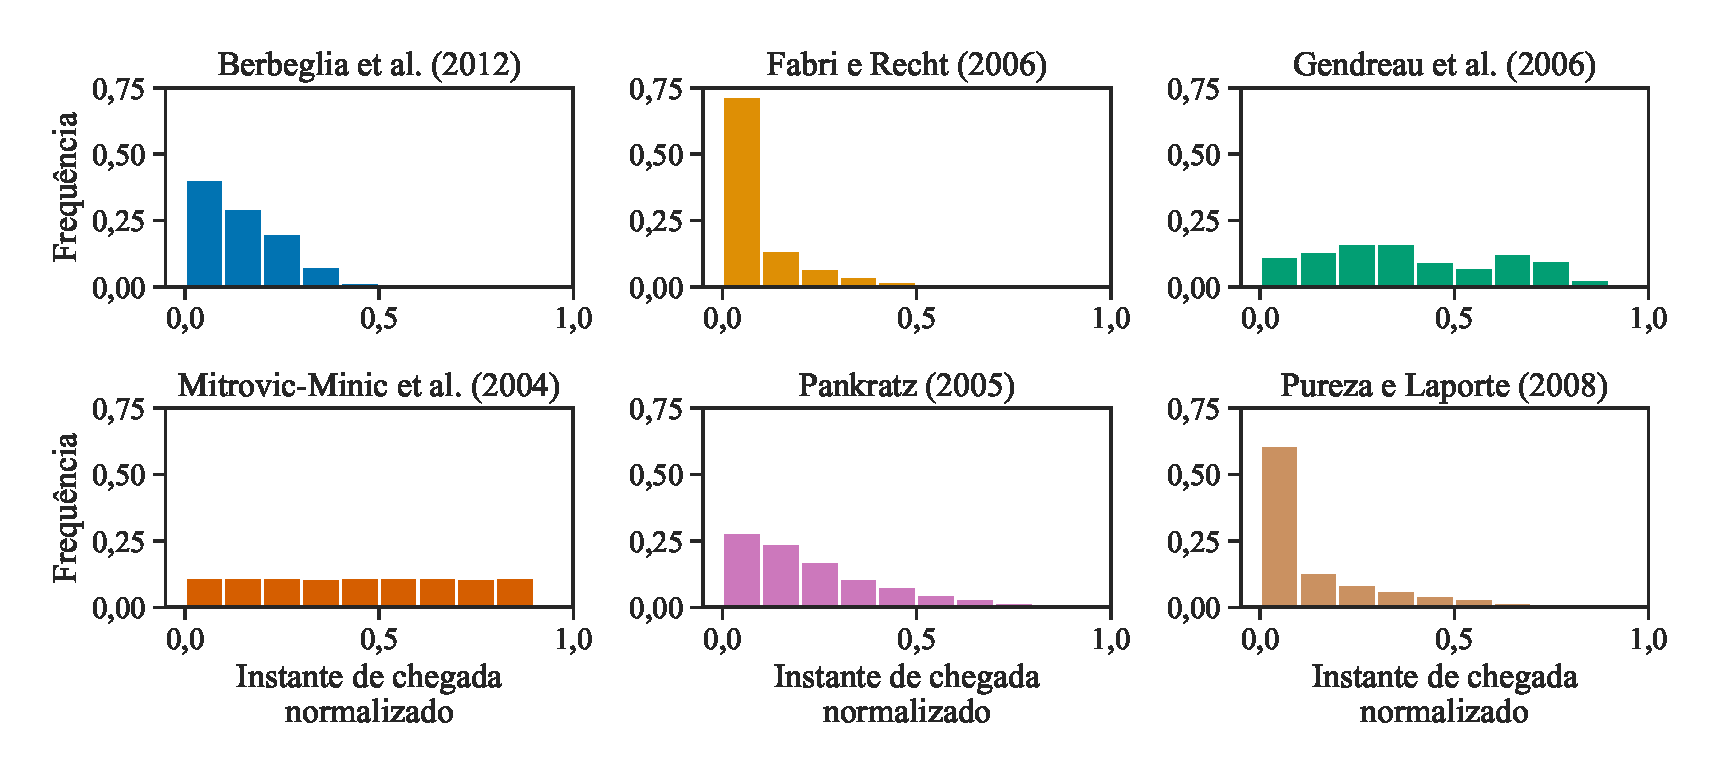
\includegraphics[width=\textwidth]
    {fig/analyses/hist_arrival_time_norm_h_by_benchmark_planing_horizon.eps}}
    \caption{Histograma dos instantes de chegada para cada conjunto 
             de \textit{benchmark}}
    \label{fig:hist_arrival_time}
\end{figure}

A Tabela~\ref{tab:correlation_real_pltw_norm_h_and_arrival_time_norm_h} 
apresenta, os valores dos coeficientes de correlação de Pearson entre os 
instantes de chegada dos pedidos e os limites inferiores das janelas de tempo 
de coleta dos pedidos.
Percebe-se uma correlação alta (maior que 0{,}75) para as instâncias de 
\citeonline{berbeglia_hybrid_tabu_2012}, 
\citeonline{mitrovic-minic_waiting_2004}, 
\citeonline{pankratz_dynamic_2005}, 
\citeonline{pureza_laporte_waiting_2008} e
\citeonline{fabri_dynamic_2006}.
Já o conjunto proposto por \citeonline{gendreau_neighborhood_2006} 
possuem uma correlação média (menor que 0{,}75) entre estes dois parâmetros, 
que pode ser explicada pelo uso de variáveis aleatórias de 
distribuição uniforme no processo de dinamização ou criação das instâncias.


\begin{table}[H]
    \footnotesize
    \centering
    \caption{Valores de correlação entre os instantes de chegadas normalizados
             e os limites inferiores normalizados das janelas de tempo de
             coleta}
    \label{tab:correlation_real_pltw_norm_h_and_arrival_time_norm_h}
    \begin{tabular}{lr}
        \toprule
        Conjunto de \textit{benchmark}                  & $r$ \\ 
        \midrule
        \citeonline{berbeglia_hybrid_tabu_2012}         & 0,95 \\
        \citeonline{fabri_dynamic_2006}                 & 0,78 \\
        \citeonline{gendreau_neighborhood_2006}         & 0,73 \\
        \citeonline{mitrovic-minic_waiting_2004}        & 1,00 \\
        \citeonline{pankratz_benchmark_2009}            & 0,81 \\
        \citeonline{pureza_laporte_waiting_2008}        & 0,89 \\ 
        \bottomrule
    \end{tabular}
\end{table}


Destaca-se que estes valores de correlação são relativos a uma relação linear
entre as variáveis em questão. Ou seja, ainda podem existir outras relações não
lineares entre o instante de chegada do pedido e o limite inferior da janela
de tempo de coleta.

As Figuras~\ref{fig:scatterplot_pickup_lower_tw_x_arrival_time}~e
\ref{fig:scatterplot_pickup_upper_tw_x_arrival_time} apresentam, 
de forma visual, as correlações entre os instantes de chegada dos 
pedidos e os limites inferiores e superiores das janelas de tempo de coleta 
dos pedidos.
Percebe-se uma correlação alta para as instâncias de 
\citeonline{berbeglia_hybrid_tabu_2012}, 
\citeonline{mitrovic-minic_double-horizon_2004}, 
\citeonline{pankratz_benchmark_2009} e 
\citeonline{pureza_laporte_waiting_2008}.
Já os conjuntos propostos por \citeonline{gendreau_neighborhood_2006} e
\citeonline{fabri_dynamic_2006} possuem uma correlação baixa entre estes 
dois valores, que pode ser explicada pelo uso de variáveis aleatórias de 
distribuição uniforme no processo de dinamização das instâncias.

% TODO Rodrigo: Explicar melhor a última frase do parágrafo anterior

\begin{figure}[h]
    \centering
    \makebox[\textwidth]
    {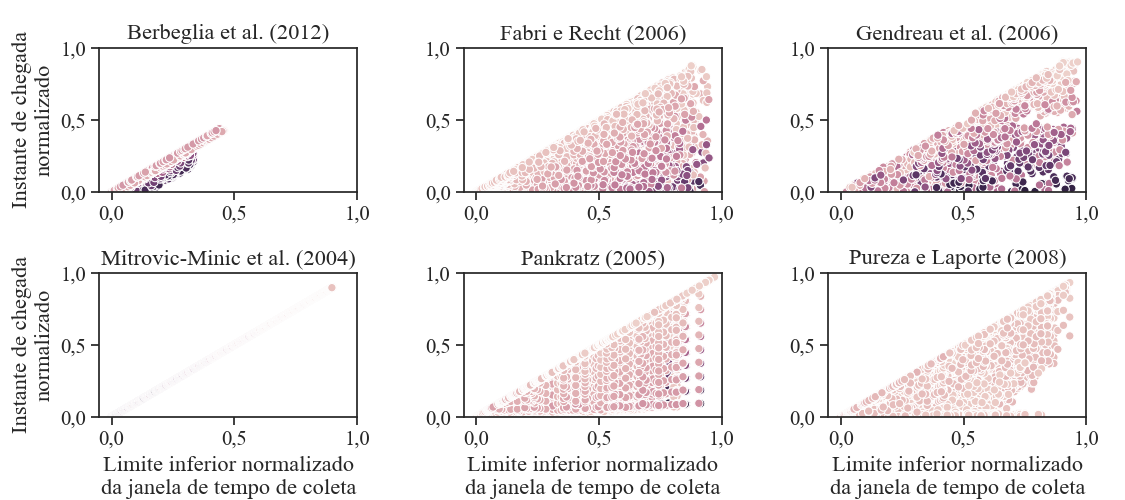
\includegraphics[width=\textwidth]
    {fig/analyses/facetgrid_scatterplot_real_pltw_norm_h_x_arrival_time_norm_h_planing_horizon.eps}}
    \caption{Gráfico de dispersão entre o limite inferior da janela de tempo
             de coleta e o instante de chegada do pedido para cada conjunto 
             de \textit{benchmark}}
    \label{fig:scatterplot_pickup_lower_tw_x_arrival_time}
\end{figure}

\begin{figure}[h]
    \centering
    \makebox[\textwidth]
    {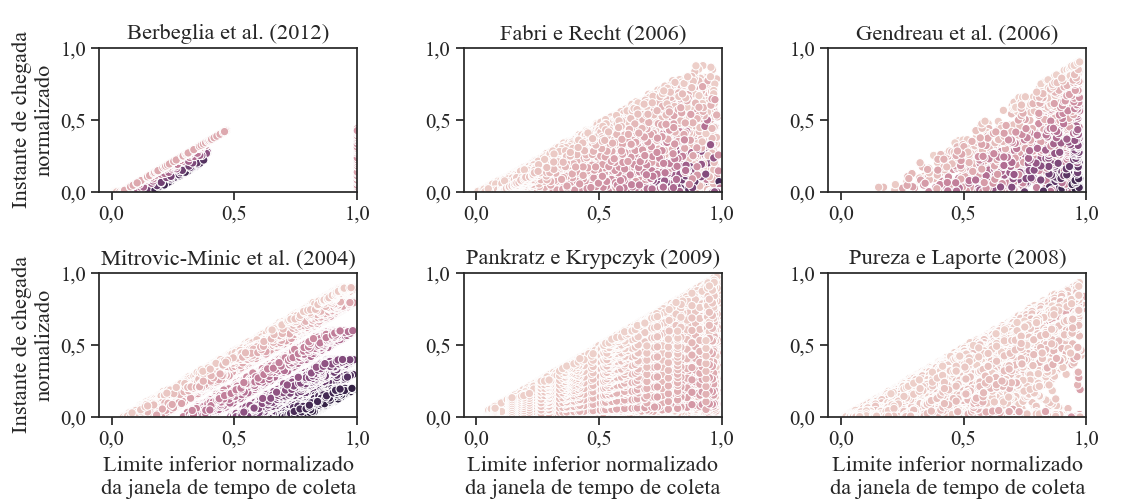
\includegraphics[width=\textwidth]
    {fig/analyses/facetgrid_scatterplot_putw_norm_h_x_arrival_time_norm_h_planing_horizon.eps}}
    \caption{Gráfico de dispersão entre o limite superior da janela de tempo 
             de coleta e o instante de chegada do pedido para cada conjunto 
             de \textit{benchmark}}
    \label{fig:scatterplot_pickup_upper_tw_x_arrival_time}
\end{figure}

Nas Figuras~\ref{fig:scatterplot_pickup_lower_tw_x_arrival_time} 
e \ref{fig:scatterplot_pickup_upper_tw_x_arrival_time} a coloração dos
pontos varia de acordo com o valor da urgência deles.
Pode-se perceber que na 
Figura~\ref{fig:scatterplot_pickup_upper_tw_x_arrival_time} 
pontos mais afastados do centro tem uma coloração mais
escura, menos urgente, que pontos próximos ao centro.
Essa é uma característica espera, tendo em vista que a urgência é dada pelo
cálculo da diferença entre o limite superior da janela de tempo de coleta e do
instante de chegada do pedido.
Já a Figura~\ref{fig:scatterplot_pickup_lower_tw_x_arrival_time} não obedece a
mesma regra.
O comportamento similar entre alguns dos gráficos apresentados nestas figuras
se deve ao fato da janela de tempo de coleta ser criada através de um método
não diversificado, gerando limites superiores e inferiores igualmente
espaçados.
Esta característica das janelas de tempo levam os conjuntos de instâncias a não
possuírem uma variação entre o tamanho das janelas de tempo, o que pode
enviesar os experimentos feitos nessas instâncias.




\section{Presença de pedidos estáticos}

A análise dos valores dos instantes de chegada de cada conjunto mostra que 
nos conjuntos propostos por \citeonline{berbeglia_hybrid_tabu_2012,
fabri_dynamic_2006, pureza_laporte_waiting_2008} uma proporção considerável 
de pedidos (mais que 10\%) chega no instante zero e, por definição, 
são considerados pedidos estáticos.
A Tabela~\ref{tab:percentage_arrival_time_equal_0} mostra a porcentagem de 
pedidos com instante de chegada igual a zero para cada um dos conjuntos de
\textit{benchmark}.

Acredita-se que este efeito colateral seja também causado pelo uso de métodos de
dinamização baseado nos limites da janela de tempo de entrega e coleta aliado ao
uso de instâncias estáticas que apresentam uma distribuição acumulada destes 
valores, principalmente no início do horizonte de planejamento.
Portanto, ao usar-se os métodos de dinamismo deve-se ter cuidado para que estes
não gerem demasiados pedidos estáticos, o que pode atrapalhar a análise de
algoritmos feitos para atender pedidos dinâmicos.

Destaca-se que esses pedidos estáticos podem também representar
uma condição inicial ao sistema. Mesmo assim, é importante perceber que alguns
métodos de geração de instâncias dinâmicas possuem uma maior probabilidade de
gerar condições iniciais com maior número de pedidos estáticos.

\begin{table}[h]
  \footnotesize
  \centering
  \caption{Porcentagem de pedidos com instante de chegada igual a zero}
  \label{tab:percentage_arrival_time_equal_0}
  \begin{tabular}{lr}
    \toprule
    Conjunto de \textit{benchmark}                  & \% \\
    \midrule
    \citeonline{berbeglia_hybrid_tabu_2012}         & 10,0 \\
    \citeonline{fabri_dynamic_2006}                 & 20,3 \\
    \citeonline{gendreau_neighborhood_2006}         &  0,7 \\
    \citeonline{mitrovic-minic_double-horizon_2004} &  0,3 \\
    \citeonline{pankratz_benchmark_2009}            &  0,0 \\
    \citeonline{pureza_laporte_waiting_2008}        & 19,5 \\ 
    \bottomrule
  \end{tabular}
\end{table}






\iffalse
\subsection{Atrelamento entre grau de dinamismo e urgência}
A urgência é calculada pela diferença entre o limite 
superior da janela de tempo da coleta e o instante de chegada do pedido, em 
muitos dos métodos de dinamização apresentados, é calculado
usando a janela de tempo de coleta como principal parâmetro.
Isso pode acarretar em um atrelamento dos valores de urgência e de dinamismo,
tendo em vista que ambos são gerados a partir da janela de tempo de coleta.
Na \autoref{fig:scatterplot_pickup_lower_tw_x_arrival_time} a coloração dos
pontos indica o valor da urgência de cada pedido, sendo pedidos menos
urgentes representados por tons claros e pedidos mais urgentes por tons
escuros.
Observa-se que nos conjuntos de \textit{benchmark} propostos por
\textcite{berbeglia_hybrid_tabu_2012, 
fabri_dynamic_2006, 
mitrovic-minic_waiting_2004, 
pankratz_dynamic_2005}
a coloração dos pontos varia juntamente com os valores dos eixo vertical 
(instante de chegada do pedido) e dos eixos horizontais (limite inferior da 
janela de tempo de coleta).
Em seu artigo, \textcite{van_lon_measures_2016} afirma que as medidas de
grau de dinamismo e urgência devem ser ortogonais, portanto, uma instância
que possua um grau de dinamismo pode possuir qualquer valor de urgência.
Portanto, os métodos de dinamização estudados possuem uma dificuldade de 
gerar cenários que cubram todo o espectro de possíveis pares de valores entre
dinamismo e urgência.
\fi


    % Finaliza a parte no bookmark do PDF para que se inicie o bookmark na raiz
    % e adiciona espaço de parte no Sumário
    %\phantompart

    % Conclusão (outro exemplo de capítulo sem numeração e presente no sumário)
    \chapter{Conclusão}\label{ch:conclusao}

% TODO Rodrigo: qual a importância de dinamismo e urgência?

Este documento apresentou, de forma detalhada, conjuntos de instâncias de 
\textit{benchmark} para o DDARP e o DPDPTW e analisou os métodos usados para a 
distribuição temporal dos instantes de chegadas dos pedidos usando, para isso,
as méticas di dinamismo e urgência propostas por 
\citeonline{van_lon_measures_2016}.

Através dessa análise, observou-se que os conjuntos possuem pouca 
variabilidade em relação aos valores de dinamismo e urgência, principalmente 
devido ao baixo número de instâncias, ao uso de métodos de dinamização simples 
e devido ao uso de instâncias estáticas com janelas de tempo de coleta
acumuladas no início do horizonte de planejamento.

Espera-se que este artigo sirva de base para demais pesquisadores da área de 
roteamento dinâmico de veículos que tenham interesse de estudar o comportamento
de algoritmos de solução para o DDARP e DPDPTW através de simulações 
computacionais de cenários diversificados.
Todos os dados das instâncias estudadas neste artigo estão disponíveis para 
consulta e utilização, assim como todos o código usado para a análise das 
instâncias \cite{eccel_problemas_2019}.

Para trabalhos futuros, recomenda-se a aplicação dos métodos de dinamização
propostos em diferentes instâncias estáticas, desse modo possibilitando uma
melhor comparação do que é influência gerada pelo próprio método e o que é 
gerado pelas características das instâncias estáticas.
Outra proposta interessante é uma análise dos fatores espaciais das 
instâncias, com relação a distribuição dos locais de coleta e entrega dos 
pedidos.


    % ELEMENTOS PÓS-TEXTUAIS
    \postextual
    \setlength\beforechapskip{0pt}
    \setlength\midchapskip{15pt}
    \setlength\afterchapskip{15pt}

    % Referências bibliográficas
    \begingroup
        % https://tex.stackexchange.com/questions/163559/how-to-modify-line-spacing-per-entry-of-bibliography
        % \linespread{1.18}\selectfont

        % https://tex.stackexchange.com/questions/17128/using-bibtex-to-make-a-list-of-references-without
        % \nocite{*}
        \printbibliography[title=REFERÊNCIAS]
    \endgroup

    % Glossário, consulte o manual da classe abntex2 para orientações sobre o glossário.
    % \ifforcedinclude\else\glossary\fi

    % Inicia os apêndices
%    \begin{apendicesenv}
        % Imprime uma página indicando o início dos apêndices
%        \ifforcedinclude\else\partapendices\fi
%        \setlength\beforechapskip{50pt}
%        \setlength\midchapskip{20pt}
%        \setlength\afterchapskip{20pt}

%        


%
% How to fix the Underfull \vbox badness has occurred while \output is active on my memoir chapter style?
% https://tex.stackexchange.com/questions/387881/how-to-fix-the-underfull-vbox-badness-has-occurred-while-output-is-active-on-m
%

% ---

\lang
{\chapter[Page not filled]{Since this page is not being completely filled, it is generating the bottom bottom of the page}}
{\chapter[Página não gerada]{Como esta página não está sendo completamente preenchida, ele está gerando a caixa inferior inferior da página}}
% ---


% Multiple-language document - babel - selectlanguage vs begin/end{otherlanguage}
% https://tex.stackexchange.com/questions/36526/multiple-language-document-babel-selectlanguage-vs-begin-endotherlanguage
\begin{otherlanguage*}{english}

\englishword{\showfont}

1. How to display the font size in use in the final output,
2. How to display the font size in use in the final output,
3. How to display the font size in use in the final output,
4. How to display the font size in use in the final output,
5. How to display the font size in use in the final output,
6. How to display the font size in use in the final output,
7. How to display the font size in use in the final output,
8. How to display the font size in use in the final output,
9. How to display the font size in use in the final output,


% As this page is not being completely filled, it is generating the page bottom bad box.
% Fix Underfull \vbox (badness 10000) has occurred while \output is active
%
% \flushbottom vs \raggedbottom
% https://tex.stackexchange.com/questions/65355/flushbottom-vs-raggedbottom
\newpage



\section[Some encoding tests]{\englishword{\showfont}}

1. How to display the font size in use in the final output,
2. How to display the font size in use in the final output,
3. How to display the font size in use in the final output,
4. How to display the font size in use in the final output,
5. How to display the font size in use in the final output,
6. How to display the font size in use in the final output,

7. How to display the font size in use in the final output,
8. How to display the font size in use in the final output,
9. How to display the font size in use in the final output,
10. How to display the font size in use in the final output,
11. How to display the font size in use in the final output,
12. How to display the font size in use in the final output,

\subsection{\englishword{\showfont}}

1. How to display the font size in use in the final output,
2. How to display the font size in use in the final output,
3. How to display the font size in use in the final output,
4. How to display the font size in use in the final output,
5. How to display the font size in use in the final output,
6. How to display the font size in use in the final output,

7. How to display the font size in use in the final output,
8. How to display the font size in use in the final output,
9. How to display the font size in use in the final output,
10. How to display the font size in use in the final output,
11. How to display the font size in use in the final output,
12. How to display the font size in use in the final output,

\subsubsection{\englishword{\showfont}}

1. How to display the font size in use in the final output,
2. How to display the font size in use in the final output,
3. How to display the font size in use in the final output,
4. How to display the font size in use in the final output,
5. How to display the font size in use in the final output,
6. How to display the font size in use in the final output,

7. How to display the font size in use in the final output,
8. How to display the font size in use in the final output,
9. How to display the font size in use in the final output,
10. How to display the font size in use in the final output,
11. How to display the font size in use in the final output,
12. How to display the font size in use in the final output,

\subsubsubsection{\englishword{\showfont}}

1. How to display the font size in use in the final output,
2. How to display the font size in use in the final output,
3. How to display the font size in use in the final output,
4. How to display the font size in use in the final output,
5. How to display the font size in use in the final output,
6. How to display the font size in use in the final output,
7. How to display the font size in use in the final output,

8. How to display the font size in use in the final output,
9. How to display the font size in use in the final output,
10. How to display the font size in use in the final output,
11. How to display the font size in use in the final output,
12. How to display the font size in use in the final output,


Lipsum me [31-35]

\end{otherlanguage*}



%    \end{apendicesenv}

%    % Inicia os anexos
%    \begin{anexosenv}
%        % Imprime uma página indicando o início dos anexos
%        \ifforcedinclude\else\partanexos\fi
%        \setlength\beforechapskip{50pt}
%        \setlength\midchapskip{20pt}
%        \setlength\afterchapskip{20pt}
%
%        

%
% How to fix the Underfull \vbox badness has occurred while \output is active on my memoir chapter style?
% https://tex.stackexchange.com/questions/387881/how-to-fix-the-underfull-vbox-badness-has-occurred-while-output-is-active-on-m
%

% ----------------------------------------------------------
\chapter{\lang{Article published in SOBRAEP magazine}{Artigo publicado}}
% ----------------------------------------------------------


% Multiple-language document - babel - selectlanguage vs begin/end{otherlanguage}
% https://tex.stackexchange.com/questions/36526/multiple-language-document-babel-selectlanguage-vs-begin-endotherlanguage
\begin{otherlanguage*}{english}

% An environment for setting \emergencystretch locally
% https://tex.stackexchange.com/questions/84510/an-environment-for-setting-emergencystretch-locally
{
    \setlength{\emergencystretch}{10pt}
    \section[English guidelines for publication]
    {English guidelines for publication - TITLE HERE (14 PT TYPE SIZE, UPPERCASE, BOLD, CENTERED)}
}
    \noindent\textbf{Abstract:}
    The objective of this document is to instruct the authors about the preparation of the
    manuscript for its submission to the Revista Eletrônica de Potência (Brazilian Power Electronics
    Journal).~The authors should use these guidelines for preparing both the initial and final
    versions of their paper. Additional information about procedures and guidelines for publication
    can be obtained directly with the editor, or through the web site
    \url{http://www.sobraep.org.br/revista}. This text was written according to these guidelines

\end{otherlanguage*}

% What is a “Overfull \hbox (9.89561pt too wide)”?
% https://tex.stackexchange.com/questions/111948/what-is-a-overfull-hbox-9-89561pt-too-wide
interwordspace: \the\fontdimen2\font

interwordstretch: \the\fontdimen3\font

emergencystretch: \the\emergencystretch\par\relax


\modifiedincludepdf{-}{ArtigoSOBRAEP}{pictures/SOBRAEP.pdf}{0.9}



%        


%
% How to fix the Underfull \vbox badness has occurred while \output is active on my memoir chapter style?
% https://tex.stackexchange.com/questions/387881/how-to-fix-the-underfull-vbox-badness-has-occurred-while-output-is-active-on-m
%

% ----------------------------------------------------------
\lang
{\chapter[Sample example]{How to display the font size in use in the final output}}
{\chapter[Anexo exemplo]{Como exibir o tamanho da fonte em uso na saída final}}
% ----------------------------------------------------------


% Multiple-language document - babel - selectlanguage vs begin/end{otherlanguage}
% https://tex.stackexchange.com/questions/36526/multiple-language-document-babel-selectlanguage-vs-begin-endotherlanguage
\begin{otherlanguage*}{english}

\englishword{\showfont}

1. How to display the font size in use in the final output,
2. How to display the font size in use in the final output,
3. How to display the font size in use in the final output,


\section[Some encoding tests]{\englishword{\showfont}}

1. How to display the font size in use in the final output,
2. How to display the font size in use in the final output,
3. How to display the font size in use in the final output,
4. How to display the font size in use in the final output,
5. How to display the font size in use in the final output,
6. How to display the font size in use in the final output,

7. How to display the font size in use in the final output,
8. How to display the font size in use in the final output,
9. How to display the font size in use in the final output,
10. How to display the font size in use in the final output,
11. How to display the font size in use in the final output,
12. How to display the font size in use in the final output,

\subsection{\englishword{\showfont}}

1. How to display the font size in use in the final output,
2. How to display the font size in use in the final output,
3. How to display the font size in use in the final output,
4. How to display the font size in use in the final output,
5. How to display the font size in use in the final output,
6. How to display the font size in use in the final output,

7. How to display the font size in use in the final output,
8. How to display the font size in use in the final output,
9. How to display the font size in use in the final output,
10. How to display the font size in use in the final output,
11. How to display the font size in use in the final output,
12. How to display the font size in use in the final output,

\subsubsection{\englishword{\showfont}}

1. How to display the font size in use in the final output,
2. How to display the font size in use in the final output,
3. How to display the font size in use in the final output,
4. How to display the font size in use in the final output,
5. How to display the font size in use in the final output,
6. How to display the font size in use in the final output,

7. How to display the font size in use in the final output,
8. How to display the font size in use in the final output,
9. How to display the font size in use in the final output,
10. How to display the font size in use in the final output,
11. How to display the font size in use in the final output,
12. How to display the font size in use in the final output,

\subsubsubsection{\englishword{\showfont}}

1. How to display the font size in use in the final output,
2. How to display the font size in use in the final output,
3. How to display the font size in use in the final output,
4. How to display the font size in use in the final output,
5. How to display the font size in use in the final output,
6. How to display the font size in use in the final output,
7. How to display the font size in use in the final output,

8. How to display the font size in use in the final output,
9. How to display the font size in use in the final output,
10. How to display the font size in use in the final output,
11. How to display the font size in use in the final output,
12. How to display the font size in use in the final output,


Lipsum me [55-65]

\end{otherlanguage*}



%    \end{anexosenv}

    % INDICE REMISSIVO
    \ifforcedinclude\else
        \phantompart
        \printindex
    \fi

\end{document}

